\documentclass[11pt,          % font size: 11pt or 12pt
               ms,            % degree:    ms or phd
               onehalfspacing % spacing: onehalfspacing or doublespacing
               ]{ncsuthesis}

%%----------------------------------------------------------------------------%%
%%------------------------------ Import Packages -----------------------------%%
%%----------------------------------------------------------------------------%%

\usepackage{booktabs}  % professionally typeset tables
\usepackage{amsmath}%,amssymb,amsfonts}
\usepackage{textcomp}  % better copyright sign, among other things
\usepackage{lipsum}    % filler text
\usepackage{subfig}    % composite figures

% user defined packages
\usepackage{algorithm}
\usepackage[noend]{algpseudocode}
\usepackage{csvsimple}
\usepackage{threeparttable}

%%%%%%%%%%%%%%%%%%%%%%%%%%%%%%%%%%%%%%%%%%
%%%%%%%%%%% Hack for alphanumeric bibliography
%%%%%%%%%%%%%%%%%%%%%%%%%%%%%%%%%%%%%%%%%%5
\RequirePackage[
			style=alphabetic,%numeric-comp,%authoryear-comp,%
			sorting=nyt,%ynt					
			hyperref=true, %	
			giveninits=true,%
			backend=bibtex,
			natbib=true,
			url=false,
			isbn=false,
			maxnames=2, %for et al to be used
			maxalphanames=1, %to avoid printing a + for every et al in abbreviation
			doi=false]{biblatex}		
			
%needed to do et al after two names
%http://tex.stackexchange.com/questions/44048/use-et-al-in-biblatex-custom-style
\renewcommand*{\finalnamedelim}{\addspace\&\space}

%Simplify abbreviation (the default uses either one or two authors and it 
%indicates et al with a +) The following five lines make it so that only the 
%first author is used in the abbreviation
%http://tex.stackexchange.com/questions/27956/label-only-from-first-author
\renewcommand*{\labelalphaothers}{}
    \renewcommand*{\intitlepunct}{}
    \DefineBibliographyStrings{english}{in={}}
    \DeclareNameAlias{sortname}{last-first}
    \DeclareNameAlias{default}{last-first}
	
\DeclareFieldFormat[article,periodical]{volume}{\mkbibbold{#1}}
\makeatletter

\newrobustcmd*{\parentexttrack}[1]{%
  \begingroup
  \blx@blxinit
  \blx@setsfcodes
  \blx@bibopenparen#1\blx@bibcloseparen
  \endgroup}

\AtEveryCite{%
  \let\parentext=\parentexttrack%
  \let\bibopenparen=\bibopenbracket%
  \let\bibcloseparen=\bibclosebracket}

\makeatother
\renewcommand{\cite}[1]{\parencite{#1}}

\renewbibmacro{in:}{%
  \ifentrytype{article}{}{%
  \printtext{\bibstring{in}\intitlepunct}}}
  
\AtEveryBibitem{\clearfield{month}}

\AtEveryBibitem{\clearfield{language}}

%%%%%%%%%%%%%%%%%%%%%%%%%%%%%%%%%%%%%%%%%%%%%

\addbibresource{WilliamDawn-thesis.bib}
\addbibresource{Mendeley.bib}
 \defbibheading{myheading}[BIBLIOGRAPHY]{
 \chapter*{#1}
 \markboth{#1}{#1}}

%amssymb and amsfonts cannot be used in conjunction with mdput
%\usepackage{amsmath,amssymb,amsfonts}
\usepackage{dcolumn}% Align table columns on decimal point
\usepackage{bm}% bold math
%\usepackage{hyperref}% add hypertext capabilities
%\usepackage{hypernat}% make hyperref and natbib work together
\usepackage{cancel}
\usepackage{verbatim}% multiline commenting
\usepackage{ifthen}
\usepackage{url}
\usepackage{sectsty}
\usepackage{balance} 
%\usepackage{caption}
\usepackage{graphicx} %eps figures can be used instead
\usepackage{lastpage}
\usepackage[format=plain,
  justification=RaggedRight,
  singlelinecheck=false,
  font=small,labelfont=bf,
  labelsep=space]{caption} 
\usepackage{fancyhdr}
\pagestyle{fancy}

%http://tex.stackexchange.com/questions/100817/error-when-using-bc-from-abbrevs-in-caption
%Getting BC
\usepackage{abbrevs}
\usepackage{etoolbox}
\robustify{\DateMark} % after having loaded abbrevs

%Needed to solve bug from citation Hydrodynamics in 21/2 dimensions
\usepackage{units}
%see http://www.latex-community.org/viewtopic.php?f=5&t=989

\usepackage[sharp]{easylist} %used for brainstorming purposes 
% used for \Asterisk for convolution %conflicts with \widering
%\usepackage{mathabx}

%compile on single pass
%\usepackage[backend=biber,...]{biblatex}

%%%%%%%%%%%%
%%% Hack to make chapters start on odd pages
% http://tex.stackexchange.com/questions/73591/how-to-have-a-blank-even-page-before-every-chapter
%%%%%%%%%%%%
%\newcommand{\ensureoddstart}{\checkoddpage\ifoddpage\else\newpage\mbox{}\fi}
%\newcommand{\ensureoddstart}{}

%%%Fancy tables
%http://tex.stackexchange.com/questions/94032/fancy-tables-in-latex
\usepackage[table]{xcolor}
\usepackage{array,booktabs}
\usepackage{colortbl}
\newcolumntype{L}{@{}>{\kern\tabcolsep}l<{\kern\tabcolsep}}

%%%%%%%%%%
%%%%% Hack to allow more levels in outline
%%%%%%%%%%
%\setcounter{secnumdepth}{5}
%\setcounter{tocdepth}{5} %may violate ETD
%Usage http://pleasemakeanote.blogspot.com/2010/06/how-to-activate-subsubsubsection-in.html
%\section{} % level 1
%\subsection{} % level 2
%\subsubsection{} % level 3
%\paragraph{} % level 4 - equivalent to subsubsubsection
%\subparagraph{} % level 5

%http://tex.stackexchange.com/questions/60209/how-to-add-an-extra-level-of-sections-with-headings-below-subsubsection
\usepackage{titlesec}

\setcounter{secnumdepth}{4}

\titleformat{\paragraph}
{\normalfont\normalsize\bfseries}{\theparagraph}{1em}{}
\titlespacing*{\paragraph}
{0pt}{3.25ex plus 1ex minus .2ex}{1.5ex plus .2ex}

%%%%%%%%%%%%%%%%%%%%%%%%%%
%%%% Hack for containing figures within sections
%%%%%%%%%%%%%%%%%%%%%%%%%%%%
%http://ctan.org/pkg/placeins
\usepackage[section]{placeins}
%Defines a \FloatBarrier command, beyond which floats may not pass; useful,
%for example, to ensure all floats for a section appear before the next 
%\section command.
% section option enforces float barriers at sections but NOT sub....sections

%%%Hack for centering all figures
%\makeatletter
%\g@addto@macro\@floatboxreset\centering
%\makeatother

%%----------------------------------------------------------------------------%%
%%---------------------------- Formatting Options ----------------------------%%
%%----------------------------------------------------------------------------%%
%%

%% -------------------------------------------------------------------------- %%
%% Disposition format -- any titles, headings, section titles
%%  These formatting commands affect all headings, titles, headings,
%%  so sizing commands should not be used here.
%%  Formatting options to consider are
%%     +  \sffamily - sans serif fonts.  Dispositions are often typeset in
%%                    sans serif, so this is a good option. 
%%     +  \rmfamily - serif fonts
%%     +  \bfseries - bold face
%\dispositionformat{\sffamily\bfseries}   % bold and sans serif
\dispositionformat{\bfseries}            % bold and serif

%% -------------------------------------------------------------------------- %%
%% Formatting for centered headings - Abstract, Dedication, etc. headings
%%  This is where one might put a sizing command.
%%  \MakeUppercase can be used to typeset all headings in uppercase.
\headingformat{\large\MakeUppercase}   % All letters uppercase
%\headingformat{\large}                % Not all uppercase
%\headingformat{\Large\scshape}        % Small Caps, used with serif fonts.

%% Typographers recommend using a normal inter-word space after
%% sentences. TeX's default is to add an wider space, but \frenchspacing
%% gives a normal spacing. Comment out the following line if you prefer
%% wider spaces between sentences.
\frenchspacing

%% -------------------------------------------------------------------------- %%
%%  Optional packages
%%    A number of compatible packages to improve the look and feel of
%%    your document are available in the file optional.tex 
%%    (For example, hyperlinks, fancy chapter headings, and fonts)
%% To use these options, uncomment the next line and see optional.tex
%%  Optional Packages to consider.   These packages are compatible with
%%    ncsuthesis.  

%% -------------------------------------------------------------------------- %%
%% Fancy chapter headings
%%  available options: Sonny, Lenny, Glenn, Conny, Rejne, Bjarne
% \usepackage[Conny]{fncychap}
\usepackage[Rejne]{fncychap}

%%----------------------------------------------------------------------------%%
%% Hyperref package creates PDF metadata and hyperlinks in Table of Contents
%%  and citations.  Based on feedback from the NCSU thesis editor, 
%%  the links are not visually distinct from normal text (i.e. no change
%%  in color or extra boxes).
\usepackage[
  pdfauthor={William C. Dawn},
  pdftitle={SFR with FEM Multiphysics},
  pdfcreator={pdftex},
  pdfsubject={NC State ETD Thesis},
  pdfkeywords={nuclear, sodium, fast, reactor, nuclear reactor, 
    finite element, multiphysics},
  colorlinks=true,
  linkcolor=black,
  citecolor=black,
  filecolor=black,
  urlcolor=black,
]{hyperref}


%% -------------------------------------------------------------------------- %%
%% Microtype - If you use pdfTeX to compile your thesis, you can use
%%              the microtype package to access advanced typographic
%%              features.  By default, using the microtype package enables
%%              character protrusion (placing glyphs a hair past the right 
%%              margin to make a visually straighter edge)
%%              and font expansion (adjusting font width slightly to get 
%%              more favorable justification).
%%              Using microtype should decrease the number of lines
%%              ending in hyphens.
\usepackage{microtype}


%%----------------------------------------------------------------------------%%
%% Fonts 

%% ETD guidelines don't specify the font.  You can enable the fonts
%%  by uncommenting the appropriate lines.  Using the default Computer 
%%  Modern fonts is *not* required.  A few common choices are below.
%%  See http://www.tug.dk/FontCatalogue/ for more options.

%% Serif Fonts -------------------------------------------------
%%  The four serif fonts listed here (Utopia, Palatino, Kerkis,
%%  and Times) all have math support.


%% Utopia
%\usepackage[T1]{fontenc}
%\usepackage[adobe-utopia]{mathdesign}

%% Palatino
%\usepackage[T1]{fontenc}
%\usepackage[sc]{mathpazo}
%\linespread{1.05}

%% Kerkis
%\usepackage[T1]{fontenc}
%\usepackage{kmath,kerkis}

%% Times
\usepackage[T1]{fontenc}
\usepackage{mathptmx}
\usepackage{amsmath}


%% Sans serif fonts -------------------------

% this will work with math and text
%\renewcommand{\familydefault}{\sfdefault}
%\usepackage[scaled]{helvet}  % Helvetica
%\usepackage[cm]{sfmath}

%\usepackage[scaled]{berasans} % Bera Sans

%solve bug from fancyhdr in optional
%http://nw360.blogspot.com/2006/11/latex-headheight-is-too-small.html
\setlength{\headheight}{14pt}

%%----------------------------------------------------------------------------%%
%%---------------------------- Content Options -------------------------------%%
%%----------------------------------------------------------------------------%%
%% Size of committee: 3, 4, 5, or 6 -- this number includes the chair
\committeesize{4}

%% Members of committee
%%  Each of the following member commands takes an optional argument
%%   to specify their role on the committee.
%%  For co-chairs, use the commands:
%%      \cochairI{Doug Dodd}
%%      \cochairII{Chris Cox}
%%
\cochairI{Scott P. Palmtag}
\cochairII{David J. Kropaczek}
\memberI{Joseph M. Doster}
\memberII{Zhilin Li}

%% Student writing thesis, \student{First Middle}{Last}
\student{William C.}{Dawn}

%% Degree program
\program{Nuclear Engineering}

%% Thesis Title
%%  Keep in mind, according to ETD guidelines:
%%    +  Capitalize first letter of important words.
%%    +  Use inverted pyramid shape if title spans more than one line.
%%
%%  Note: To break the title onto multiple lines, use \break instead of \\.
%\thesistitle{A North Carolina State University Sample \LaTeX{} Thesis \break 
%with a Title So Long it Needs a Line Break}
\thesistitle{Sodium Cooled Fast Reactor Simulations with the Finite Element
Method}

%% Degree year.  Necessary if your degree year doesn't equal the current year.
%\degreeyear{1995}

%%----------------------------------------------------------------------------%%
%%---------------------------- Personal Macros -------------------------------%%
%%----------------------------------------------------------------------------%%

%% A central location to add your favorite macros.
%% user defined commands and macros

%% A few examples to get you started.
\newcommand{\uv}[1]{\ensuremath{\mathbf{\hat{#1}}}}
\newcommand{\bo}{\ensuremath{\mathbf{\Omega}}}
% \renewcommand{\exp}[1]{e^{#1}}
\newcommand{\Conv}{\mathop{\scalebox{1.5}{\raisebox{-0.2ex}{$\ast$}}}}%

% linear algebra
%    vectors
\newcommand{\va}{\mathbf{a}}
\newcommand{\vb}{\mathbf{b}}
\newcommand{\vc}{\mathbf{c}}
\newcommand{\vd}{\mathbf{d}}
\newcommand{\ve}{\mathbf{e}}
\newcommand{\vf}{\mathbf{f}}
\newcommand{\vn}{\mathbf{n}}
\newcommand{\vp}{\mathbf{p}}
\newcommand{\vr}{\mathbf{r}}
\newcommand{\vu}{\mathbf{u}}
\newcommand{\vx}{\mathbf{x}}
\newcommand{\vw}{\mathbf{w}}
%    matrices
\newcommand{\ma}{\mathbf{A}}
\newcommand{\mj}{\mathbf{J}}
\newcommand{\ml}{\mathbf{L}}
%    sets
\newcommand{\real}{\mathbb{R}}
\newcommand{\realn}{\real^{n}}
\newcommand{\realnn}{\real^{n \times n}}

% variable definitions
\newcommand{\keff}{k_{\!\mbox{\scriptsize \em eff}}}
\newcommand{\kref}{k_{\!\mbox{\scriptsize \em ref}}}
\newcommand{\grad}{\mathbf{\nabla}}

% general macros
\newcommand{\units}[1]{\;\text{[{#1}]}}

% neutronDiffusion
\newcommand{\albedo}{\alpha}
\newcommand{\basis}{N}
\newcommand{\twotable}{TwoTable }
\newcommand{\phiavg}{\overline{\phi}}
\newcommand{\mcc}{MC**2}

\newcommand{\half}{\frac{1}{2}}

% reference macros
\newcommand{\eref}[1]{Eq.~\ref{#1}}
\newcommand{\fref}[1]{Fig.~\ref{#1}}
\newcommand{\tref}[1]{Table~\ref{#1}}
\newcommand{\sref}[1]{Sec.~\ref{#1}}
\newcommand{\chref}[1]{Chapter ~\ref{#1}}
\newcommand{\apref}[1]{Appendix ~\ref{#1}}

\usepackage{color}
\newcommand{\NEW}[1]{#1}
\newcommand{\COMMENT}[1]{\textcolor{green}{#1}}

\newcommand{\NOTER}[1]{\textcolor{orange}{#1}}
\newcommand{\NOTEC}[1]{\textcolor{blue}{#1}}
\newcommand{\NOTEK}[1]{\textcolor{magenta}{#1}}

\newcommand{\mum}{\ensuremath{{\mu}\text{m}}}

%This makes it so that you can add short paths in your .tex by including the
%folders where you store your images in the search path
\graphicspath{
  {./ch01_introduction/figs/}
  {./ch02_neutronDiffusion/figs/}
  {./ch03_thermalExpansion/figs/}
  {./ch04_thermalHydraulics/figs/}
  {./ch05_conclusions/figs/}
  {./apA_analyticSolutions/figs/}
  {./apB_benchmarks/figs/}
  }

%%---------------------------------------------------------------------------%%
\usepackage{calc}
%% Capital letter height
\newlength{\chaptercapitalheight}
\settoheight{\chaptercapitalheight}{D}
\newlength{\chapterfootskip}
\setlength{\chapterfootskip}{\chaptercapitalheight}
\addtolength{\chapterfootskip}{2\baselineskip}
% A little extra space to ensure there are 2 full double spaced lines
\addtolength{\chapterfootskip}{0.5ex}
%\def\chapterfootskipnum{\chapterfootskip}
\renewcommand{\listfigurename}{LIST OF FIGURES}
\renewcommand{\listtablename}{LIST OF TABLES}
\renewcommand{\bibname}{BIBLIOGRAPHY}

%\renewcommand{\cfttoctitlefont}{\centering\ncsu@headingformat}

%http://tex.stackexchange.com/questions/47184/height-of-figure-caption-textheight
\newlength\graphht
\newcommand\calculategraphicstargetheight[1]{%
     \setlength\graphht{\textheight 
                       -\parskip
                       -\abovecaptionskip -\belowcaptionskip
                       -(12pt * #1) % assuming baselineskip of 12pt in caption
                       -\chapterfootskip
                       }}
%\usepackage{titlesec}

%landscape support in fancyhdr from 
%http://tex.stackexchange.com/questions/9071/how-to-translate-and-rotate-the-heading-of-landscaped-pages
\usepackage{pdflscape}
\usepackage{tikz}
\fancypagestyle{lscapedplain}{%
  \fancyhf{}
  \fancyfoot{%
    \tikz[remember picture,overlay]
      \node[outer sep=1cm,above,rotate=90] at (current page.east) {\thepage};}
\renewcommand{\headrulewidth}{0pt} 
\renewcommand{\footrulewidth}{0pt}
}

\begin{document}
\pagestyle{plain}
%%---------------------------------------------------------------------------%%
\frontmatter
%% ------------------------------ Abstract ---------------------------------- %%
\begin{abstract}
  Renewed interest in advanced nuclear power reactors such as the Versatile Test 
  Reactor (VTR) at Idaho National Laboratory (INL) has encouraged enhanced 
  modeling of Sodium Cooled Fast Reactors (SFRs). Since their inception in the 
  early days of nuclear engineering with reactors such as at the Experimental 
  Breeder Reactor and Fermi 1, many new modeling techniques have been developed.
  This work seeks to introduce cutting-edge methods to the simulation of SFRs.

  In this work, the multigroup neutron diffusion equation is solved via the
  Finite Element Method (FEM). This method allows for the use of unstructured
  and general meshes. By using an unstructured mesh, physical phenomena such as
  thermal expansion can be modeled and used to perturb the mesh. Additionally,
  the FEM will allow for simplified mesh refinements by means of both geometric
  refinement and the use of higher order methods without recreating the mesh.
  The multigroup neutron diffusion equation can be solved for two-dimensional
  problems using triangles or three-dimensional problems using pentahedra, also
  known as wedges. 

  Thermal feedback effects within a SFR are also modeled in this work. A
  simplified thermal hydraulic model is used, modeling both axial heat 
  convection and radial heat conduction. Resulting temperatures are used to 
  calculate on-the-fly neutron cross-sections to capture the effects of Doppler
  feedback. Additionally, a thermal expansion model is used to simulate the 
  thermal expansion of fuel and structural components within the reactor. These 
  effects have been proven to significantly impact reactor behavior in 
  experiments such as those performed at Experimental Breeder Reactor II 
  (EBR-II).

  Using these models, a typical SFR is simulated at operating conditions. The 
  models as implemented demonstrate expected reactor behavior for an SFR and can
  be used to visualize the inherent safety features and feedback effects of such 
  a nuclear reactor.
  
\end{abstract}

%% ---------------------------- Copyright page ------------------------------ %%
\makecopyrightpage

%% -------------------------------- Title page ------------------------------ %%
\maketitlepage

%% -------------------------------- Dedication ------------------------------ %%
\begin{dedication}
  \centering To the future of clean electricity and natural beauty.
\end{dedication}

%% -------------------------------- Biography ------------------------------- %%
\begin{biography}
  William C. Dawn was born and raised in Stafford, Virginia. He attended public
  schools there for his primary education, participating in the Commonwealth
  Governor's School for High School. William earned a B.S. degree in Nuclear
  Eneingeering from North Carolina State University (NC State) in May 2017. 
  After his Master's degree, William will remain at NC State to pursue a Ph.D.
  degree in Nuclear Engineering. 

  William is a fellow of the Integrated University Program (IUP) facilitated by
  DOE-NE. During his undergraduate and graduate careers, he has had the
  opportunity to work with GE-Hitachi Nuclear Energy LLC. and Oak Ridge National
  Laboratory (ORNL). William has also made contributions to the Consortium for
  Advanced Simulation of LWRs (CASL).
\end{biography}

%% ----------------------------- Acknowledgements --------------------------- %%
\begin{acknowledgements}
  This work would not have been possible without the help of friends and family.
  I would like to thank my Mom and Dad, Suzanne and Bill Dawn, for their
  patience, their listening, and their advice. Their support has helped to make
  this work a reality.

  I would also like to thank my advisor, Dr. Scott Palmtag. We have both learned
  tremendously during this process. His consistency and desire to know more have
  kept me busy these last few months and I am grateful.
\end{acknowledgements}

%% ----------------------------- Disclaimer --------------------------- %%
\clearpage
\vspace*{\fill}
\begin{center}
  \mbox{\parbox{5in}{
  This material is based upon work supported under an Integrated
  University Program Graduate Fellowship. Any opinions, findings, conclusions,
  or recommendations expressed in this publication are those of the author and
  do not necessarily reflect the views of the Department of Energy Office of
  Nuclear Energy.
  }}
\end{center}
\vspace*{\fill}
\clearpage

\thesistableofcontents

\thesislistoftables

\thesislistoffigures

%%---------------------------------------------------------------------------%%
\mainmatter

\pagestyle{plain}
\newgeometry{margin=1in,lmargin=1.25in,footskip=\chapterfootskip, includehead, 
  includefoot}
\chapter{Introduction}
\label{ch:introduction}

\section{Motivation}
  Recent interest in advanced and next-generation nuclear power reactor designs
  has encouraged further development of modeling and simulation methods for
  these reactors. Fast reactors, a class of advanced reactors, operate with
  predominately high-energy (``fast'') neutrons in the fission reaction. Since
  early development of fast reactors, such as  \gls{ebr-i} in 1951 and Fermi 1
  in 1956, there have been significant innovations in both nuclear modeling and
  computational methods. As development of fast reactors is revisited in the
  form of the \gls{vtr} at \gls{inl}, improvements in simulation can be
  used to simulate fast reactors with modern best practices. 
  

  Nuclear reactor simulations are inherently multiphysics simulations. For
  example, neutron reaction probabilities are described by cross sections.
  Neutron cross sections are dependent on material temperatures and densities,
  both of which vary over the operating range of a nuclear power reactor. As
  reactor power changes, material temperatures and densities change, therefore
  cross sections change and affect the reactor power. The multiphysics nature
  of the reactor necessitate a simulation of the power distribution within the
  reactor as well as all feedback effects which will be modeled. 
  
  In this thesis, models for simulating fast reactors will be developed and
  demonstrated. Reactor power distribution will be modeled according to the
  multigroup neutron diffusion equation as solved by the \gls{fem} based on
  unstructured meshes with special attention to hexagonal geometries.
  The multigroup neutron diffusion solution method is verified through
  comparison to both benchmark and analytic solutions. Multiphysics effects are
  modeled including thermal hydraulics and thermal expansion. Thermal hydraulic
  effects are modeled as axial heat convection and radial heat conduction.
  Thermal expansion is modeled using simplified linear expansion models. The
  methods developed in this work can easily be used for fast reactors with a
  variety of coolants including sodium, lead, or molten salt.

  By employing a modern solution method to the neutron diffusion equation in the
  form of the \gls{fem}, the simulation can take advantage of developments in
  numerical methods including the solution of linear systems. Additionally, the
  simulation allows for the incorporation of generalized multiphysics effects
  whereas current state-of-the-art techniques (such as \dif) require data
  processing and manual iteration to simulate multiphysics effects. Ultimately, 
  the simulation is designed to simulate an operating fast reactor and estimate
  feedback coefficients by coupling multiphysics models.

\section{Geometry Description}
  \label{sec:geometry_description}
  The high-energy neutron spectra inherent to fast reactors results in
  relatively small neutron cross sections compared to larger cross sections in
  the thermal energy range. To compensate for this fact, fast reactors are
  typically designed with hexagonal, triangularly pitched, fuel assemblies to
  maximize fuel packing. An example of a fast reactor with hexagonal fuel
  assemblies is shown in \fref{fig:reactor_materials}.
  
  \begin{figure}
    \centering
    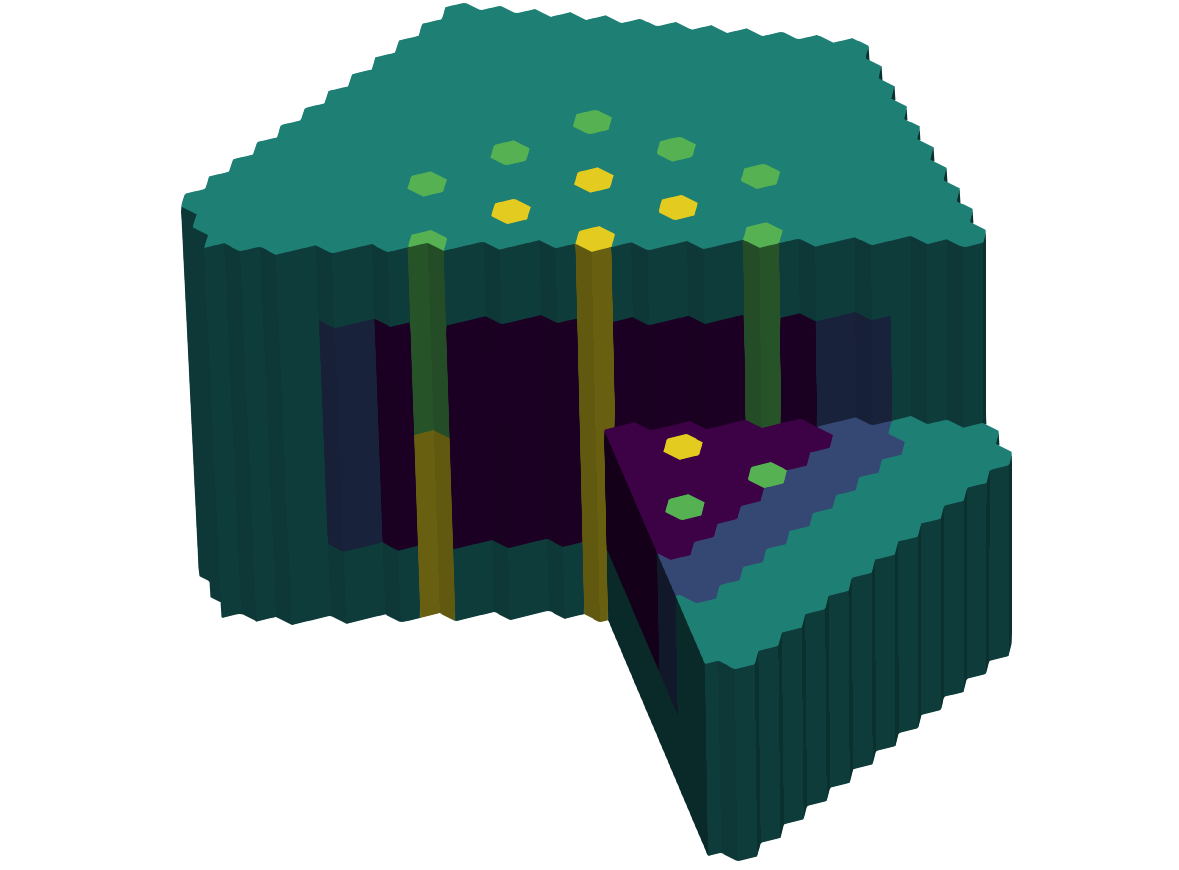
\includegraphics[width=\textwidth]{reactor_materials}
    \caption{Example of Fast Reactor Materials based on MONJU.}
    \label{fig:reactor_materials}
  \end{figure}

  \begin{figure}
    \centering
    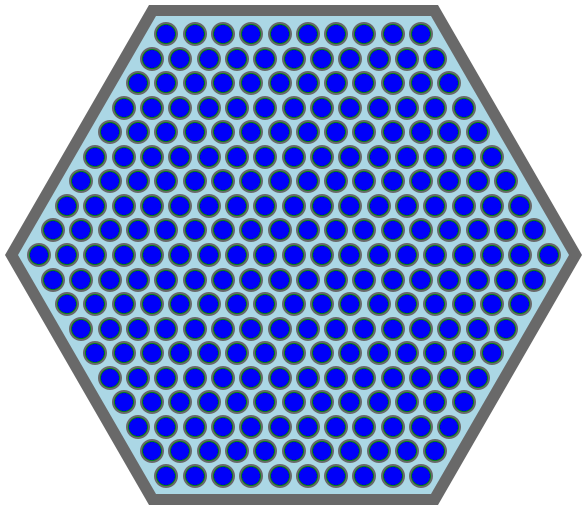
\includegraphics[width=0.5\textwidth]{prism_hex}
    \caption{Example of Fast Reactor Fuel Assembly Cross Section.}
    \label{fig:prism_hex}
  \end{figure}

  A cross-sectional representation of a hexagonal fuel assembly is shown in
  \fref{fig:prism_hex}. This geometry is used in the homogenization of neutron
  cross sections and is also used to describe coolant flow geometries.
  Dimensions of assemblies are measured at room temperature and will later be
  expanded according to the thermal expansion model in
  \chref{ch:thermalExpansion}.

  Note the individual rods in \fref{fig:prism_hex} are cylindrical and are
  arranged into a hexagonal assembly. The basic geometry is a metallic fuel
  material within stainless steel cladding. The gap between the fuel and
  cladding is filled by sodium bond to improve thermal conductivity across the
  gap. The rod is helically wrapped by a steel wire to ensure separation between
  rods that will allow for coolant flow. The wire wrap also serves to encourage
  the mixture of coolant within the assembly. (Note: wire wrap is omitted from
  \fref{fig:prism_hex}.) Many rods are then assembled into an assembly and
  surrounded by a hexagonal can made of steel. This can aids in structural
  stability and prohibits cross-flow of coolant between assemblies. 

  The dimensions within a single rod are shown in \fref{fig:pin_model} and the
  dimensions within a hexagonal assembly can are shown in \fref{fig:hex_can}. In
  \fref{fig:hex_can}, $T\!h_{can}$ is the thickness of the assembly can,
  $F\!2\!F$ is the flat-to-flat measurement of the outside of the hexagonal can,
  and \textit{Pitch} is the distance between the center of two rods. Using the
  geometry described in these figures, the material cross-sectional areas are
  calculated according to the given formulae where $N_{rod}$ is the number of
  rods in the assembly and $A\!P$ is the assembly pitch. $A\!P > F\!2\!F$ to
  account for inter-assembly sodium gaps (see ``Gap'' in \fref{fig:hex_can}).
  \begin{align}
    \label{eq:afrac_first}
    A_{total} &= \frac{\sqrt{3}}{2} A\!P^2 \\
    A_{box} &= 
      \frac{\sqrt{3}}{2} \left(F\!2\!F^2 - \left(F\!2\!F - 2
      Th_{can}\right)^2\right) \\
    A_{wrap} &= N_{rod} \frac{\pi}{4} D_{wrap}^2 \\
    A_{clad} &= N_{rod} \pi (R_C^2 - R_B^2) \\
    A_{bond} &= N_{rod} \pi (R_B^2 - R_F^2) \\
    A_{fuel} &= N_{rod} \pi R_F^2 \\
    A_{cool} &= A_{total} - A_{box} - A_{wrap} - A_{clad} - A_{bond} -
      A_{fuel}\\
    \label{eq:afrac_last}
    A_{struct} &= A_{box} + A_{wrap} + A_{clad}
  \end{align}
  Calculating the areas as above allows for calculation of cross-sectional area
  fractions. Assuming constant dimensions in the axial direction, these area
  fractions are equivalent to volume fractions and are useful for neutron
  cross section homogenization. Additionally, these formulae allow for thermal
  expansion as the liquid sodium in the bond and the liquid coolant are allowed
  to vary to allow for the expansion of other materials.

  \begin{figure}
    \centering
    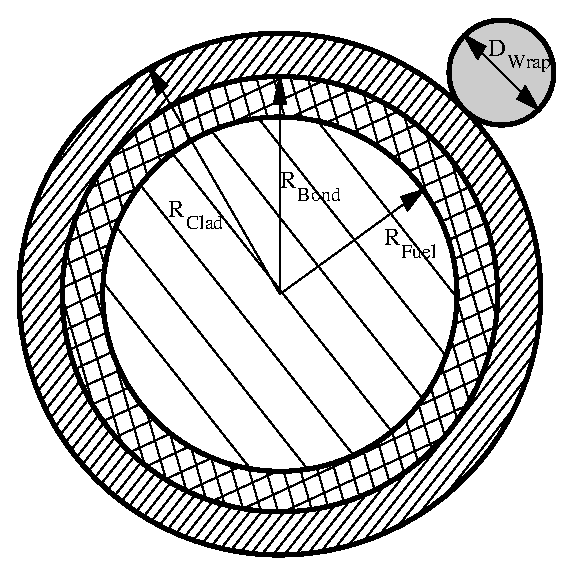
\includegraphics[width=0.6\textwidth]{pin_model}
    \caption{Dimensions of Thermal Hydraulic Rod Model (not to scale).}
    \label{fig:pin_model}
  \end{figure}

  \begin{figure}
    \centering
    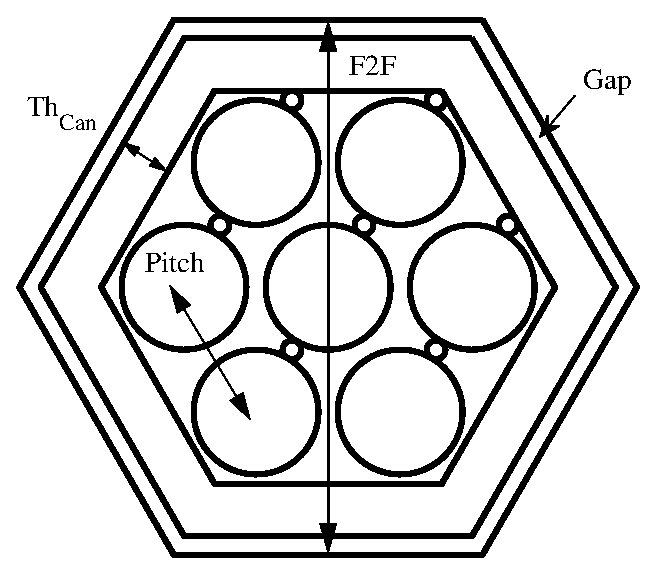
\includegraphics[width=0.6\textwidth]{hex_can}
    \caption{Dimensions of Hexagonal Can (not to scale).}
    \label{fig:hex_can}
  \end{figure}

\section{Cross Section Treatment}
  \label{sec:cross_section_treatment}
  Reactor materials are ``smeared'' into homogeneous regions. This treatment is
  common to fast reactors because of the relatively large neutron
  mean-free-paths compared to the scale of material dimensions. Additionally,
  the neutron distribution will be modeled using the neutron diffusion equation
  which cannot accurately resolve small geometric details. The natural
  choice for these homogeneous regions are the hexagonal assemblies themselves.
  Materials are permitted to be heterogeneous axially. For this work, four
  distinct regions are modeled within a hexagonal assembly: fuel, bond, coolant,
  and steel. Steel material includes cladding, wire wrap, and assembly can. 
  These four regions are then homogenized into a hexagonal assembly.

  For simplified analytic and benchmark problems, cross sections are specified
  by the problem. For realistic simulations, multigroup microscopic cross
  sections are generated using the computer program \mcc \cite{mcc}. The cross
  section generator uses 2,082 fine energy groups to collapse down to an
  arbitrary number of coarse energy groups. For this simulation, the recommended
  and default 33-group energy structure is used. However, the methods in this
  work are implemented generally and are not dependent on a particular energy
  group structure. \mcc solves the infinite-homogeneous (zero-dimension) neutron
  transport equation for isotopic number densities as input by the user.  Cross
  sections for each assembly type are generated separately to accurately
  simulate the neutron energy spectrum within the assembly. This procedure
  results in a unique material cross sections for each assembly type. For
  example, each assembly type contains steel; therefore, there will be a
  separate steel cross section for each assembly type in the cross section
  library. Within \mcc, the neutron energy spectrum for fissile media is
  generated by the media's fission spectrum.  Non-fissile homogenized mixtures,
  such as control assemblies or reflector assemblies, the default
  \isotope[238]{U} fission spectrum is assumed.

  Cross section libraries are generated for several different temperatures to
  capture temperature-dependent cross section effects. These libraries are then
  used during the simulation to calculate cross sections as a function of
  material temperatures. The fuel, clad, and coolant temperatures in a
  simulated reactor can be calculated with a thermal hydraulic model (see
  \chref{ch:thermalHydraulics}). However, the temperatures calculated in the
  thermal hydraulic model are functions of reactor power and coolant mass flow
  rate. These parameters are not known before the simulation for a general
  reactor. Instead, a simplified one-dimensional, single-channel model is used
  to estimate temperatures for cross section library generation. This model is
  based on the axial convection and radial conduction models in
  \chref{ch:thermalHydraulics}. The simulation model can use general cross
  section library temperatures and a general number of temperature libraries.
  A user may select the number of cross section libraries and specify the
  temperatures for which the libraries apply in a general manner. Typical 
  cross section library temperatures for simulating liquid metal cooled, metal
  fueled, fast reactors are given in \tref{tab:xstemps}.

  \begin{table}
    \caption{Temperatures Selected for Cross Section Libraries.}
    \label{tab:xstemps}
    \begin{center}
      \begin{tabular}{crrr}
        \toprule
        Library & $T_{cool} \units{K}$ & $T_{clad} \units{K}$ & 
          $T_{fuel} \units{K}$ \\
        \midrule
        1 & 628.15 & 628.15 & 628.15  \\
        2 & 708.65 & 757.50 & 807.15  \\
        3 & 896.87 & 920.47 & 961.46 \\
        4 & 1072.81 & 1114.83 & 1183.14 \\
        \bottomrule
      \end{tabular}
    \end{center}
  \end{table}

  Note that the maximum temperatures in \tref{tab:xstemps} are greater than 
  temperatures observed at typical reactor operating conditions. This is
  necessary so that even at perturbed reactor conditions (e.g. $110\%$ full
  power), the peak core temperatures can still be interpolated within the
  libraries.

  Cross sections are homogenized within each hexagonal assembly using isotopic
  microscopic cross sections from \mcc and user input number densities.
  Homogenization is performed in two steps: first, isotopic homogenization and
  second, volumetric homogenization. Isotopic homogenization is performed by
  summing microscopic cross sections and associated number densities. Let
  $\sigma_{i,j,x,g}$ represent the microscopic cross section for isotope $i$, in
  region $j$, for reaction type $x$, and energy group $g$ as output by \mcc.
  $\sigma_{i,j,x,g}$ has units of area. Then, let $N_{i,j}$ represent the atom
  number density for isotope $i$ in region $j$ as input by the user. $N_{i,j}$
  has units of inverse volume. The macroscopic cross section can then be
  defined
  \begin{equation}
    \label{eq:isotopic_homogenization}
    \Sigma_{j,x,g} = \sum_{i=1}^{N_{iso}} N_{i,j} \, \sigma_{i,j,x,g}
  \end{equation}
  where $\Sigma_{j,x,g}$ is the macroscopic cross section in region $j$, for
  reaction type $x$, and energy group $g$. In \eref{eq:isotopic_homogenization},
  $N_{iso}$ represents the number of isotopes in region $j$. Note that
  $\Sigma_{j,x,g}$ will have units of inverse length.

  Next, volumetric cross section homogenization is performed using volume
  fractions. Assuming dimensions do not change axially within a hexagonal
  assembly, the areas calculated in \eref{eq:afrac_first} through
  \eref{eq:afrac_last} can be used to calculate area fractions.
  These area fractions can subsequently be treated as volume fractions.
  Using the definition of macroscopic cross sections from
  \eref{eq:isotopic_homogenization}, the volumetrically homogenized macroscopic
  cross section is 
  \begin{equation}
    \label{eq:volumetric_homogenization}
    \Sigma_{x,g} = \frac{\sum_{j = 1}^{N_{reg}} \Sigma_{j,x,g} \, V_j}
      {\sum_{j=1}^{N_{reg}} V_j}
  \end{equation}
  where $V_j$ is the volume or area occupied by region $j$ in the hexagonal
  assembly and $N_{reg}$ is the number of regions in the hexagonal assembly.
  Typically, $N_{reg} = 4$ with unique regions for fuel, sodium bond, sodium
  coolant, and steel structural material. After homogenizing cross sections
  isotopically and volumetrically, the diffusion coefficient for energy group
  $g$, $D_g$, can be calculated as 
  \begin{equation}
    \label{eq:diffusion_homogenization}
    D_g = \frac{1}{3 \Sigma_{tr,g}}
  \end{equation}
  where $\Sigma_{tr,g}$ represents the macroscopic transport cross section for
  energy group $g$. $\Sigma_{tr,g}$ has been homogenized according to
  \eref{eq:isotopic_homogenization} and \eref{eq:volumetric_homogenization}.
  Note that $D_g$ will have units of length.

\section{Thesis Organization}
  In \chref{ch:neutronDiffusion}, the derivation of the \gls{fem} solution to
  the multigroup neutron diffusion equation is presented. Special attention is
  paid to triangular and wedge elements. The resulting eigenvalue problem is
  solved using the Power Method. Results from the diffusion solution are
  verified in two-dimensional and three-dimensional problems with both analytic 
  and benchmark solutions. These verification problems for the neutron diffusion
  equation are presented in \chref{ch:diffusionResults}.

  \chref{ch:thermalHydraulics} presents the formulation of axial heat convection
  and radial heat conduction models for a typical fast reactor. These models are 
  used to calculate material temperatures and update cross sections for the 
  simulation. Results of the numerical model are compared to analytical models 
  and example material temperatures are shown.

  In \chref{ch:thermalExpansion} a simplified thermal expansion model is
  presented. The model assumes linear thermal expansion for given material
  properties and user-specified thermal expansion temperatures. A simple
  demonstration of the effects of thermal expansion on reactivity are presented.

  The combination of all of these models allows for the realistic simulation of
  a fast reactor. In \chref{ch:coupledResults}, the multiphysics models are
  coupled and investigated for a benchmark reactor problem. Using this benchmark
  reactor and the models described, multiphysics reactivity feedback
  coefficients are estimated.
 
  Finally, \chref{ch:conclusions} presents a summary and the conclusions of this
  research. Additionally, recommendations for further research are provided.

\chapter{Finite Element Neutron Diffusion}
\label{ch:neutronDiffusion}

\section{Introduction}
  This chapter will describe the solution of the multigroup neutron diffusion
  equations for general geometry via the \glsentryfull{fem}. The solution method
  and derivations here are general to the multigroup neutron diffusion equation
  and its application to any standard reactor geometry is straightforward. For
  typical fast reactor applications, diffusion theory approximates the neutron
  distribution within the reactor well. The diffusion approximation is a
  standard assumption for fast reactors because neutron mean-free-paths within
  the reactor are large relative to material dimensions.

  Spatial discretization will be done with the \gls{fem}. This spatial 
  discretization method is selected for several reasons. It allows for easily 
  increasing the spatial convergence order of the method by increasing the order
  of the elements without refining the mesh. For example, with a given mesh, 
  quadratic elements instead of linear elements could be used to spatially 
  refine the solution. Additionally, coordinates of nodes and elements can be 
  easily updated to reflect physical phenomena, such as thermal expansion (see 
  \chref{ch:thermalExpansion}). Finally, material properties are calculated on 
  an element basis allowing for detailed updates to the material properties 
  during the calculation.

\section{Multigroup Neutron Diffusion Equation}
  In the multigroup neutron diffusion equation, an energy structure is 
  described by the set of energies $\{E_g\}$ for $g = 1,2,\ldots,G$.
  By convention, the energy groups are arranged in order of decreasing energy.
  \begin{equation}
    0 < E_G < E_{G-1} < \ldots < E_2 < E_1
  \end{equation}
  Multigroup neutron cross sections can be calculated using this energy group 
  structure from energy dependent cross sections, and a representative flux
  spectrum. Generation of multigroup neutron cross sections is performed using
  \mcc and is described in \sref{sec:cross_section_treatment}.

  In conventional notation, the multigroup neutron diffusion equation can be
  written as 
  \begin{equation}
    \label{eq:multigroup_diffusion}
    - \grad \cdot ( D_g(\vr) \grad \phi_g(\vr)) + \Sigma_{t,g}(\vr) \phi_g(\vr)= 
      \frac{\widetilde{\chi_g}(\vr)}{\keff} 
      \sum_{g'=1}^{G} \nu\Sigma_{f,g'}(\vr) 
      \phi_{g'}(\vr) + \sum_{g'=1}^{G} \Sigma_{s,g' \rightarrow g}(\vr) 
      \phi_{g'}(\vr)
  \end{equation}
  where 
  \begin{conditions} % custom environment designed for this purpose
    \vr & spatial position vector, \\
    D_g(\vr)    & diffusion coefficient for energy group $g$ \units{cm}, \\
    \phi_g(\vr) & scalar neutron flux for energy group $g$
      \units{$\frac{1}{\text{cm}^2 \; \text{s}}$}, \\
    \Sigma_{t,g}(\vr) & macroscopic total cross section for energy group $g$ 
      \units{$\frac{1}{\text{cm}}$}, \\
    \widetilde{\chi_g}(\vr) & effective fission spectrum for energy group $g$,\\
    \keff & effective neutron multiplication factor, \\
    \nu \Sigma_{f,g}(\vr) & number of fission neutrons times microscopic fission
      cross section in energy group $g$ \units{$\frac{1}{\text{cm}}$}, \\
    \Sigma_{s,g' \rightarrow g} (\vr) & macroscopic scatter cross section from
      energy group $g'$ to energy group $g$ \units{$\frac{1}{\text{cm}}$}, \\
    G & total number of energy groups.
  \end{conditions}

  The total neutron cross section includes the contribution due to within-group
  scattering; that is, due to $\Sigma_{s,g\rightarrow g}$. This can be
  subtracted from both sides of \eref{eq:multigroup_diffusion} for simplicity
  and numeric efficiency. Rewriting \eref{eq:multigroup_diffusion} with this
  modification yields
  \begin{equation} 
    \label{eq:multigroup_removal}
    - \grad \cdot( D_g(\vr) \grad \phi_g(\vr)) + \Sigma_{r,g}(\vr) \phi_g(\vr) = 
      \frac{\widetilde{\chi_g}(\vr)}{\keff} 
      \sum_{g'=1}^{G} \nu\Sigma_{f,g'}(\vr) 
      \phi_{g'}(\vr) + \sum_{g'=1, g' \ne g}^{G} 
      \Sigma_{s,g' \rightarrow g}(\vr) \phi_{g'}(\vr)
  \end{equation}
  where $\Sigma_{r,g}$ is the removal cross section defined as
  $\Sigma_{r,g}(\vr) = \Sigma_{t,g}(\vr) - \Sigma_{s,g\rightarrow g}(\vr)$. The
  removal cross section now describes the removal of neutrons from the element
  of phase space due to nuclear interactions.  For simplicity, the neutron
  sources in \eref{eq:multigroup_removal} can be combined into a single term as
  \begin{equation}
    \label{eq:multigroup_source}
    - \grad \cdot( D_g(\vr) \grad \phi_g(\vr)) + \Sigma_{r,g}(\vr) \phi_g(\vr) = 
      q_g(\vr)
  \end{equation}
  where $q_g(\vr)$ is the combined neutron source at position $\vr$ for energy
  group $g$ and is expressed as
  \begin{equation}
    \label{eq:q}
    q_g(\vr) = q_{fiss,g}(\vr) + q_{up,g}(\vr) + q_{down,g}(\vr) 
  \end{equation}
  with contributing terms
  \begin{align}
    \label{eq:qfiss}
    q_{fiss,g}(\vr) &= \frac{\widetilde{\chi_g}(\vr)}{\keff} \sum_{g'=1}^{G} 
      \nu \Sigma_{f,g'}(\vr) \phi_{g'}(\vr), \\
    \label{eq:qup}
    q_{up,g}(\vr) &= \sum_{g'=g+1}^{G} \Sigma_{s,g' \rightarrow g}(\vr)
      \phi_{g'}(\vr), \\
    \label{eq:qdown}
    q_{down,g}(\vr) &= \sum_{g'=1}^{g-1} \Sigma_{s,g' \rightarrow g}(\vr)
      \phi_{g'}(\vr),
  \end{align}
  where the difference between $q_{up}$ and $q_{down}$ are the limits of the
  summation. $q_{up}$ represents the neutron source due to scattering from lower
  energy groups (up-scattering) and $q_{down}$ represents the neutron source due
  to scattering from higher energy groups (down-scattering). This form allows
  for operator splitting of the neutron source term. In an iterative scheme, it
  will be necessary for fission and up-scatter sources to use a different flux
  iterate than down-scatter so this separation of sources will prove useful (see
  \sref{sec:calculation_of_source_with_power_iterations}).

  The combined source form is useful for solving the multigroup neutron
  diffusion problem for an arbitrary number of groups.
  \eref{eq:multigroup_source} is solved for each energy group and interaction
  between groups is described in the source term, $q_g(\vr)$. In other
  literature, the multigroup equation may be solved for all groups
  simultaneously by treating interaction between groups explicitly. By solving
  each group independently (as done here) the method remains general.
  Additionally, for many-group energy structures, as common to fast reactor
  applications, solving each group independently is typically more
  computationally efficient as such linear systems have favorable conditioning
  and are dimensionally smaller. Finally, fast reactors are also dominated by
  down-scatter as opposed to thermal reactors which experience significant
  up-scatter implying that the term $q_{up,g}(\vr)$ will not have to be updated
  frequently and the one group at-a-time solution method will benefit.

  Typically, reactor materials are described isotopically and $\chi$ may be
  specified isotopically. However, for calculating the fission neutron source
  $q_{fiss,g}(\vr)$ as in \eref{eq:qfiss}, an effective $\widetilde{\chi}$ is 
  needed. From an isotopic description, $q_{fiss,g}(\vr)$ is given as
  \begin{equation}
    \label{eq:isotopic_chi}
    q_{fiss,g}(\vr) = \sum_{i=1}^{N_{iso}} \chi_{i,g}(\vr)
      \nu \Sigma_{f,i,g}(\vr) \phi_g(\vr)
  \end{equation}
  where $\chi_{i,g}(\vr)$ is the isotopic fission spectrum and $N_{iso}$ is the 
  number of isotopes at position $\vr$. Next, require $q_{fiss,g}(\vr)$ to have 
  the form of \eref{eq:element_chi}.
  \begin{equation}
    \label{eq:element_chi}
    q_{fiss,g}(\vr) = \widetilde{\chi_g}(\vr) \, 
      \sum_{i=1}^{N_{iso}} \nu \Sigma_{f,i,g}(\vr) \phi_g(\vr)
  \end{equation}
  Setting \eref{eq:isotopic_chi} equal to \eref{eq:element_chi} yields the
  expression for $\widetilde{\chi_g}(\vr)$ based on isotopic data.
  \begin{equation}
    \label{eq:chi_collapse}
    \widetilde{\chi_g}(\vr) = \frac{\sum_{i=1}^{N_{iso}} \chi_{i,g}(\vr)
      \nu \Sigma_{f,i,g}(\vr) \phi_g(\vr)}
      {\sum_{i=1}^{N_{iso}} \nu \Sigma_{f,i,g}(\vr) \phi_g(\vr)}
  \end{equation}
  Note that \eref{eq:chi_collapse} requires the solution $\phi_g(\vr)$.
  Ultimately, the flux is unknown but will be solved in an iterative manner.
  \eref{eq:chi_collapse} implies that $\widetilde{\chi_g}(\vr)$ must be updated
  for each iteration of the solution (see Step \ref{state:chi_collapse} in
  \algorithmref{algorithm:general}).
  
\section{Formulation of Finite Element Equations}
  \label{sec:formulation}
  This section presents the derivation of the spatial discretization of the
  multigroup neutron diffusion equation based on the \gls{fem}. The method
  results in a linear system of equations for a fixed source iteration. Details
  are also provided on constructing the finite element matrix for use with
  triangular and wedge elements.

  \subsection{Derivation}
    \label{sec:formulation:derivation}
    The remaining continuous variable in the problem to be discretized in
    \eref{eq:multigroup_source} is the spatial variable $\vr$. This will be 
    discretized according to the \gls{fem}. The problem is solved in a finite 
    domain $\vr \in \Omega$ where $\partial \Omega$ represents the boundary of 
    the domain and some boundary condition is specified. Boundary condition 
    options include:
    \begin{enumerate}
      \item Mirror. $\grad \phi_g(\vr) \cdot \nhat = 0$ for 
        $\vr \in \partial \Omega$.
      \item Albedo. $D_g(\vr) \grad \phi_g(\vr) \cdot \nhat + 
        \albedo \phi_g(\vr)=0$ for $\vr \in \partial \Omega$,
        where $\albedo \in \real$ is a scalar constant specified
        by the user. For non-reentrant boundary condition, $\albedo = \half$.
      \item Zero Flux. $\phi_g(\vr) = 0$ for $\vr \in \partial \Omega$.
    \end{enumerate}
    $\nhat$ represents the unit outward normal vector at the boundary $\partial
    \Omega$.
    (Note: the order of the above list corresponds to the order of boundary 
    condition precedent in code with the greater the integer, the greater the 
    precedent.)
    
    Begin by partitioning the spatial domain $\Omega$ into a set of finite 
    elements.
    \begin{equation}
      \label{eq:set_of_elements}
      \Omega = \Omega_1 \cup \Omega_2 \cup \Omega_3 \cup \ldots \cup
        \Omega_{N_E} 
    \end{equation}
    such that $\Omega = \{\Omega_e\}$ for $e = 1,2,\ldots,N_E$ is a set of
    non-overlapping elements 
    \begin{equation}
      \label{eq:non_overlapping}
      \Omega_i \cap \Omega_j = \emptyset, \quad \text{for } i \ne j
    \end{equation}
    and $N_E$ is the total number of elements. Elements are in an unstructured
    mesh and can be generated by any number of mesh generation methods (e.g.
    Delaunay triangulation) to describe the geometry of the problem.
    
    Proceeding with the Galerkin \gls{fem}, \eref{eq:multigroup_source} is
    multiplied by a testing function $v(\vr) \in H_1(\Omega)$ where $H$ is the
    Sobolev space. 
    \begin{equation}
      \label{eq:testing_function_multiply}
      -\grad \cdot (D_g(\vr) \grad \phi_g(\vr)) v(\vr) + 
        \Sigma_{r,g}(\vr) \phi_g(\vr) v(\vr) =
        q_g(\vr) v(\vr)
    \end{equation}
    Then, \eref{eq:testing_function_multiply} is integrated over the problem 
    domain. This integration yields the Weak Form or Variational Form of the 
    problem.
    \begin{equation}
      \label{eq:fem_weak_form}
      - \int_{\Omega} \grad \cdot (D_g(\vr) \grad \phi_g(\vr)) v(\vr) \; d\vr
        + \int_{\Omega} \Sigma_{r,g}(\vr) \phi_g(\vr) v(\vr) \;d\vr=
        \int_{\Omega} q_g(\vr) v(\vr) \;d\vr
    \end{equation}
    
    For the purposes of this work, material cross sections and the neutron
    source, $q_{g,e}$, are assumed to be constant within an element. In the
    future, $q_g$ could be considered discrete at each node rather than each
    element. To calculate a constant neutron source within an element,
    \eref{eq:q} is used to calculate the average neutron source, $q_{g,e}$,
    in an element.
    \begin{align}
      q_{g,e} &= q_{fiss,g,e} + q_{up,g,e} + q_{down,g,e} \\
      \label{eq:chielement}
      \widetilde{\chi_{g,e}} &= \frac{\sum_{i=1}^{N_{iso}} \chi_{i,g,e}
        \nu \Sigma_{f,i,g,e} \phiavg_{g,e}}
        {\sum_{i=1}^{N_{iso}} \nu \Sigma_{f,i,g,e} \phiavg_{g,e}} \\
      \label{eq:qelement_fiss}
      q_{fiss,g,e} &= \frac{\widetilde{\chi_{g,e}}}{\keff} \sum_{g'=1}^G \nu
        \Sigma_{f,g',e} \phiavg_{g',e} \\
      \label{eq:qelement_up}
      q_{up,g,e} &= \sum_{g'=g+1}^G \Sigma_{s,g' \rightarrow g,e}
        \phiavg_{g',e}\\
      \label{eq:qelement_down}
      q_{down,g,e} &= \sum_{g'=1}^{g-1} \Sigma_{s,g' \rightarrow g,e}
        \phiavg_{g',e}
    \end{align}
    Note that in \eref{eq:chielement}, $\widetilde{\chi_{g,e}}$ must now be
    calculated for each finite element.  For first-order, linear implementations
    of the \gls{fem}, the element-average flux $\phiavg_{g,e}$ is
    \begin{equation}
      \label{eq:phiavg}
      \phiavg_{g,e} = \frac{1}{N_p} \sum_{i \in \Omega_e}^{N_p} \phi_{i,g}
    \end{equation}
    where $N_p$ is the number of nodes on the element and $i \in
    \Omega_e$ is the summation over all nodes in element $\Omega_e$. For 
    example, a triangle has $N_p = 3$ and a wedge has $N_p = 6$.

    Given constant material properties and constant neutron source over the
    element, the integrals in \eref{eq:fem_weak_form} can be partitioned into a
    sum of integrals over the elements in the domain assuming the
    non-overlapping set of elements from \eref{eq:set_of_elements} and
    \eref{eq:non_overlapping}.
    \begin{equation} 
      \label{eq:element_by_element}
      -\sum_{e=1}^{N_E} D_{g,e} 
        \int_{\Omega_e} \grad \cdot \grad \phi_g(\vr) v(\vr) \; d\vr +
        \sum_{e=1}^{N_E} \Sigma_{r,g,e} \int_{\Omega_e} \phi_g(\vr) v(\vr) 
        \;d\vr = \sum_{e=1}^{N_E} q_{g,e} \int_{\Omega_e} v(\vr) 
        \; d\vr
    \end{equation}
    The Second Green's Theorem is used to rewrite the integral in the first
    term. A proof invoking the Second Green's Theorem has been published by
    \textcite{textbookli}. % in Theorem 9.2.
    The Second Green's Theorem is 
    \begin{equation} 
      \label{eq:greens}
      -\int_{\Omega_e} \grad \cdot \grad \phi_g(\vr) v(\vr) \;d\vr =
        -\int_{\partial \Omega_e}  
        (\grad \phi_g(\vr) \cdot \nhat) \, v(\vr)\; ds +
        \int_{\Omega_e} \grad \phi_g(\vr) \cdot \grad v(\vr) \; d\vr
    \end{equation}
    where $\grad \phi_g(\vr) \cdot \nhat$ is the outward normal derivative and
    the integral $\int_{\partial \Omega} {\cdot} \;ds$ is a line integral in two
    dimensions or a surface integral in three dimensions. Recognizing that this
    quantity will only be relevant on the boundary of the problem, the value of
    the outward normal derivative will be specified as a boundary condition.
    Specifically, the albedo boundary condition which has the form 
    \begin{align}
      D_g(\vr) \grad \phi_g(\vr) \cdot \nhat + \albedo \phi_g(\vr) &= 0 \\
      D_g(\vr) \grad \phi_g(\vr) \cdot \nhat &= -\albedo \phi_g(\vr)
    \end{align}
    for $\vr \in \partial \Omega$. Note that all allowed boundary conditions
    (mirror, albedo, and zero-flux) can be specified as an albedo condition. For
    mirror boundaries, $\albedo = 0$ and for zero-flux boundaries, $\albedo
    \rightarrow \infty$.  Substituting \eref{eq:greens} into
    \eref{eq:element_by_element} and assuming the outward normal derivative is
    specified in the form of an albedo boundary condition with $\albedo$
    constant throughout the problem boundary.
    \begin{multline} 
      -\sum_{e=1}^{N_E} D_{g,e} \int_{\partial \Omega_e} v(\vr) \grad
      \phi_g(\vr) \cdot \nhat \;ds + \sum_{e=1}^{N_E} 
        D_{g,e} \int_{\Omega_e} \grad \phi_g(\vr) \cdot \grad v(\vr) 
        \; d\vr + \\
        \sum_{e=1}^{N_E} \Sigma_{r,g,e} \int_{\Omega_e} \phi_g(\vr) v(\vr) 
        \; d\vr =
        \sum_{e=1}^{N_E} q_{g,e} \int_{\Omega_e} v(\vr) \; d\vr
    \end{multline}
    \begin{multline}
      \label{eq:element_boundary}
      \sum_{e=1}^{N_E} \albedo \int_{\partial \Omega_e} v(\vr) 
        \phi_g(\vr) \;ds + \sum_{e=1}^{N_E} D_{g,e}
        \int_{\Omega_e} \grad \phi_g(\vr) \cdot \grad v(\vr) \; d\vr + \\
        \sum_{e=1}^{N_E} \Sigma_{r,g,e} \int_{\Omega_e} \phi_g(\vr) v(\vr) 
        \; d\vr =
        \sum_{e=1}^{N_E} q_{g,e} \int_{\Omega_e} v(\vr) \; d\vr
    \end{multline}
    Next, for the Galerkin formulation of the \gls{fem}, the function of
    interest $\phi_g(\vr)$ is assumed to be a linear combination of chosen basis
    functions, $\basis_i$, as
    \begin{equation} 
      \label{eq:linear_combination}
      \phi_g(\vr) = \sum_{i=1}^{DOF} \upsilon_{i,g} \, \basis_i(\vr)
    \end{equation}
    where coefficients $\vu_g = \{\upsilon_{i,g}\}$ are unknown and will be 
    determined and $DOF$ is the total number degrees of freedom of the problem. 
    Typically $DOF$ is the number of nodes less any nodes for which the flux is 
    fixed (e.g. zero-flux nodes). 
    
    Typically, basis functions have unit magnitude and are centered at the node
    points so the coefficients $\upsilon_{i,g}$ are the \gls{fem} solution at the
    nodes. It is also convenient for basis functions to have compact support.
    That is, basis functions are created such that they are zero almost
    everywhere except some minimal region. Compact support in this
    implementation is chosen such that basis functions have unit value on a
    single mesh node and are zero on all other mesh nodes. Basis functions are
    typically piecewise continuous polynomials of arbitrary degree. For selected
    elements, basis functions will be defined explicitly in
    \sref{sec:matrix_quantities}. Linear and quadratic polynomials are common;
    but, for the work presented here, only linear basis functions are explored.

    The test function, $v(\vr) \in H_1(\Omega)$, is also chosen as a linear 
    combination of the same basis functions.
    \begin{equation} 
      \label{eq:linear_superposition}
      v(\vr) = \sum_{j=1}^{DOF} \basis_j(\vr)
    \end{equation}
    The magnitude of the testing function is arbitrary so the magnitude is set
    to unity.
    
    \eref{eq:linear_combination} and \eref{eq:linear_superposition} are inserted 
    into \eref{eq:element_boundary}.
    \begin{multline}
      \label{eq:this_above}
      \sum_{e=1}^{N_E} \albedo \sum_{i=1}^{DOF} \upsilon_{i,g}
        \int_{\partial \Omega_e}
        \basis_i(\vr)  \basis_j(\vr) \;ds +
        \sum_{e=1}^{N_E} D_{g,e} \sum_{i=1}^{DOF} \upsilon_{i,g}
        \int_{\Omega_e} \grad \basis_i(\vr) \cdot \grad \basis_i(\vr)\;d\vr
        + \\
        \sum_{e=1}^{N_E} \Sigma_{r,g,e} \sum_{i=1}^{DOF} \upsilon_{i,g}
        \int_{\Omega_e} \basis_i(\vr) \basis_j(\vr) \; d\vr =
        \sum_{e=1}^{N_E} q_{g,e} \sum_{i=1}^{DOF} 
        \int_{\Omega_e} \basis_i(\vr) \; d\vr
    \end{multline}
    \eref{eq:this_above} can be rearranged as a linear system of equations.
    \begin{multline}
      \label{eq:linear_equation}
      \sum_{i=1}^{DOF} \upsilon_{i,g} \sum_{j=1}^{DOF} \left(
        \sum_{e=1}^{N_E} \albedo \int_{\partial \Omega_e}
        \basis_i(\vr)  \basis_j(\vr) \;ds +
        \sum_{e=1}^{N_E} D_{g,e} 
        \int_{\Omega_e} \grad \basis_i(\vr) \cdot \grad \basis_j(\vr)\;d\vr
        \right.
        + \\
        \left.
        \sum_{e=1}^{N_E} \Sigma_{r,g,e}
        \int_{\Omega_e} \basis_i(\vr) \basis_j(\vr) \; d\vr \right) =
        \sum_{i=1}^{DOF} \left(
        \sum_{e=1}^{N_E} q_{g,e} 
        \int_{\Omega_e} \basis_i(\vr) \; d\vr \right)
    \end{multline}
    Which can be written in the notation common to the mathematical discussions 
    of the \gls{fem}
    \begin{equation}
      \label{eq:fem_notation}
      a_g(\basis_i,\basis_j) = f_g(\basis_i)
    \end{equation}
    where $a_g(\basis_i,\basis_j)$ is the bilinear form of the \gls{fem} for 
    group $g$ and $f_g(\basis_i)$ is the linear form of the \gls{fem} for group
    $g$.
    \eref{eq:linear_equation} can also be written in matrix format as
    \begin{equation}
      \label{eq:matrix_notation}
      \ma_g \, \vu_g = \vf_g
    \end{equation}
    where $\vu_g = \{\upsilon_{i,g}\}$. 
    
    The diffusion coefficient $D_g(\vr)$ is non-zero and bounded and the removal
    cross section $\Sigma_{r,g}(\vr)$ is bounded. Given these conditions, the
    Lax-Milgram Lemma implies the solution to the \gls{fem} equations as derived
    here is both unique and bounded \cite{textbookli}. This is not the entire
    solution description as the source function $q_g(\vr)$ is updated on each
    power iteration (see \sref{sec:power_iterations}). What the satisfaction of
    the Lax-Milgram Lemma does imply is, for a fixed source problem 
    in a given power iteration, a unique and bounded solution exists. The
    multigroup neutron diffusion problem remains an eigenvalue problem.
    
    In the matrix notation of \eref{eq:matrix_notation}, matrix $\ma_g$ is 
    described by integral quantities, vector $\vu_g$ is the unknown magnitudes 
    of the basis functions $\{\upsilon_{i,g}\}$, and vector $\vf_g$ is described
    by source integral quantities. Inspecting the elements matrix $\ma_g$ and
    the vector $\vf_g$ reveals 
    \begin{align}
      \label{eq:matrix_population}
      A_{i,j,g,e} &= \albedo \int_{\partial \Omega_e} \basis_i(\vr) 
        \basis_j(\vr) \; ds + D_{g,e} 
        \int_{\Omega_e} \grad \basis_i(\vr) \cdot \grad \basis_j(\vr) \;
        d\Omega_e + \Sigma_{r,g,e} \int_{\Omega_e} \basis_i(\vr) \basis_j(\vr)
        \; d\Omega_e, \\
      \label{eq:vector_population}
      f_{i,g,e} &= q_{g,e} \int_{\Omega_e} \basis_i(\vr) \;d\Omega_e.
    \end{align}
    Then, all element data can be combined as
    \begin{align}
      A_{i,j,g} &= \sum_{e=1}^{N_E} A_{i,j,g,e}, \\
      f_{i,g} &=  \sum_{e=1}^{N_E} f_{i,g,e},
    \end{align}
    which leads to the natural population of the matrix $\ma_g$ in an
    element-by-element procedure. Matrix $\ma_g$ is assembled by looping through
    all elements and summing their contribution to the matrix. Note that the
    contribution due to the surface integral will be zero in elements not on the
    problem boundary and may also be zero for problems with select boundary
    conditions. See \sref{sec:boundary_conditions} for boundary condition
    discussion. The population of the vector $\vf_g$ is done similarly in an
    element-by-element fashion. Then, the matrix $\ma_g$ and the vector $\vf_g$
    are known for each energy group. The equations are solved for one energy
    group at a time and $\phi_g$ is calculated and stored. 
    
    The above derivation reduces to a linear system of equations. These
    equations are constructed from the integral quantities specified by the
    \gls{fem} and the coefficients given by the cross sections.  The integral
    quantities themselves are expressed explicitly in the
    \sref{sec:matrix_quantities}.
    
  \subsection{Matrix Quantities}
    \label{sec:matrix_quantities}
    For selected simple elements, the integral quantities described in 
    \eref{eq:matrix_population} and \eref{eq:vector_population} have exact 
    analytic forms. For this work, linear triangles and linear wedges
    are investigated and many of the integrals have exact expressions. If these 
    quantities cannot be expressed exactly, or doing so would be computationally
    inefficient, numerical quadratures are used. Given proper selection of
    the quadrature set, a quadrature rule can express the integrals exactly. 
    This will be discussed in \sref{sec:quadratures}.

    \subsubsection{Linear Triangles}
      Linear triangles are common to two-dimensional \glspl{fem} and have been
      investigated in many methods for the solution of the few-group neutron
      diffusion equation \cite{Hosseini2017,Hosseini2013,Hosseini2015}.
      The linear triangle element is a triangle defined by three corner
      coordinates with basis functions located on each corner. 

      \begin{figure}
        \centering
        \subfloat[General Triangle Element.]
          {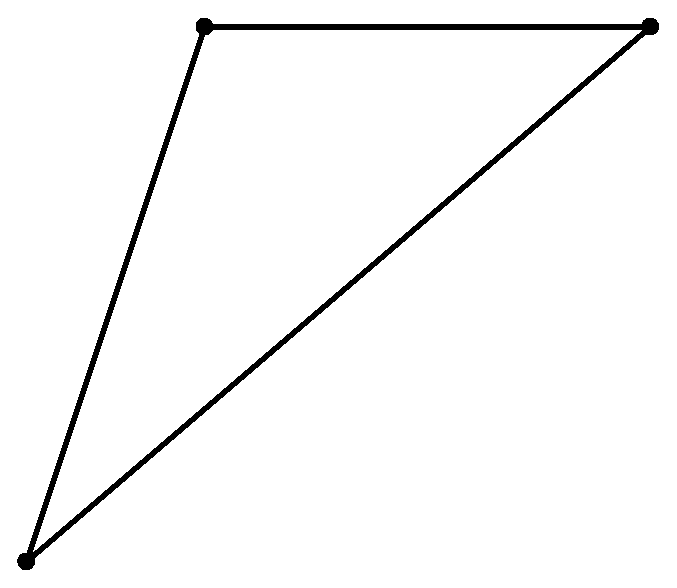
\includegraphics[width=0.35\textwidth]{sketch_triangle}}
        \vspace{0.2in}
        \subfloat[Reference Triangle.]
          {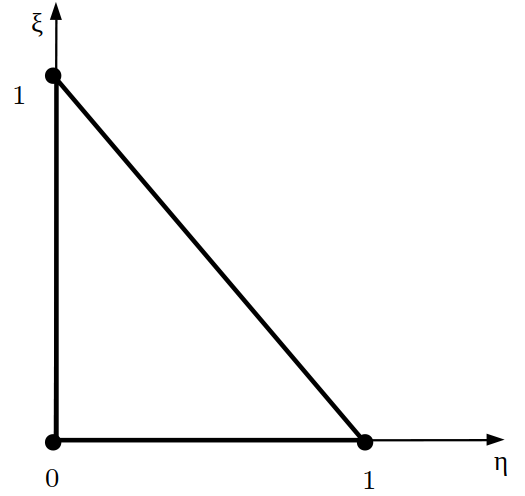
\includegraphics[width=0.35\textwidth]{Tref}}
        \caption{Description of Triangle Elements.}
        \label{fig:triangle_elements}
      \end{figure}

      It is difficult to analytically calculate the desired integral quantities
      for an arbitrary triangle. Instead, a simplified reference element is
      created and quantities are calculated for the reference element and then
      translated to the arbitrary element using a Jacobian.  The reference
      triangle $T_{ref}$ is located in $\xi \in [0,1]$ and $\eta \in [0,1-\xi]$.
      General and reference triangles are shown in \fref{fig:triangle_elements}.
      The basis functions are zero outside of the reference triangle. Within
      the reference triangle, basis functions for the are provided in the
      natural coordinates of $T_{ref}$.
      \begin{align}
        \basis_i(\xi,\eta) &= 0 \quad \forall \; (\xi,\eta) \notin T_{ref} \\
        \basis_1(\xi,\eta) &= \xi \\
        \basis_2(\xi,\eta) &= \eta \\
        \basis_3(\xi,\eta) &= 1-\xi-\eta
      \end{align}
      
      For linear triangles, simple expressions for the integral quantities for
      an arbitrary triangle can be derived \cite{textbookwhite}. The expression
      for the line integral for the arbitrary element can also be derived
      \cite{computerLab}. For a general triangle with corners $( x_i,y_i )$ with
      $i=1,2,3$
      \begin{align}
        \int_{\Omega_e} \grad \basis_i(\vr) \cdot \grad \basis_j(\vr) 
          \;d\vr &= \frac{1}{4 A_e}
          ((x_{i+1}-x_{i+2})(x_{j+1}-x_{j+2}) + 
          (y_{i+1}-y_{i+2})(y_{j+1}-y_{j+2})), \\
        \int_{\Omega_e} \basis_i(\vr) \basis_j(\vr) \;d\vr &= 
          \frac{A_e}{12} (1+\delta_{ij}), \\
        \int_{\Omega_e} \basis_i(\vr) \;d\vr &= \frac{A_e}{3}, \\
        \int_{\partial \Omega_e} \basis_i(\vr) \basis_j(\vr) \;ds &=
          \frac{L_e}{6}(1+\delta_{ij}), 
      \end{align}
      where $A_e$ is the area of the triangular element, $L_e$ is the length of 
      the edge between node $i$ and node $j$, and $\delta_{ij}$ is the Kronecker
      delta.
      The Kronecker delta is defined as
      \begin{equation} \label{eq:kroneker_delta}
        \delta_{ij} =
        \begin{cases}
          0 & \text{if } i \ne j, \\
          1 & \text{if } i = j.
        \end{cases}
      \end{equation}
      The area of a triangle in three dimensions is calculated for a triangle
      with corner coordinates $\vc_i = (x_i, y_i, z_i)$ with $i=1,2,3$.
      That is, $\vc_i$ is the coordinates of corner $i$. Calculation of the area
      of a general triangle is then given by the vector operations
      \begin{align}
        \va &= \vc_2 - \vc_1, \\
        \vb &= \vc_3 - \vc_1, \\
        A_e &= \half \lvert \va \times \vc \rvert, \\
        \label{eq:area_triangle}
        A_e &= \half \sqrt{ (a_2 b_3 - a_3 b_2)^2 + (a_3 b_1 - a_1 b_3)^2 +
          (a_1 b_2 - a_2 b_1)^2},
      \end{align}
      where $a_i$ is the $i^{th}$ component of vector $\va$ and $b_i$ is the
      $i^{th}$ component of vector $\vb$.  For higher order triangular elements
      (e.g. quadratic or cubic elements), it may be necessary to employ a
      quadrature to calculate the necessary integral quantities.

    \subsubsection{Linear Wedges}
      A wedge element is a pentahedron with six corner nodes, and is sometimes
      referred to as a triangular prism. A simple example of a wedge is an
      extruded triangle. However, unlike an extruded triangle, the exact 
      geometric relation of corner nodes in a wedge is not fixed and the nodes 
      are free to expand and distort. An example of typical and distorted
      wedge elements are shown in \fref{fig:sketch_wedge}. These elements are
      unique because there are two different types of faces. Three faces are
      quadrilateral and two are triangular. 

      \begin{figure}
        \centering
        \subfloat[General Wedge Element.]
          {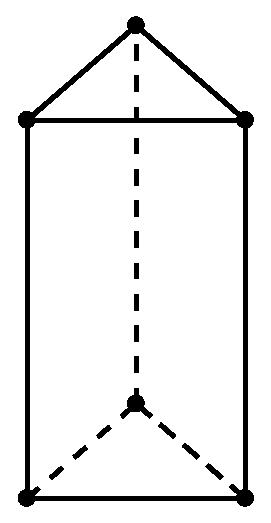
\includegraphics[width=0.2\textwidth]{wedge_sketch}}
        \vspace{0.5in}
        \subfloat[Distorted Wedge Element.]
          {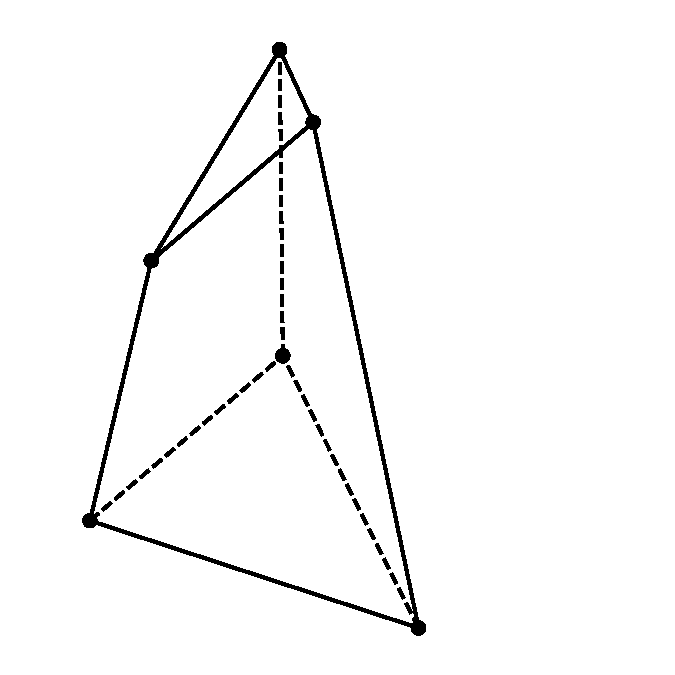
\includegraphics[width=0.2\textwidth]{wedge_stretch}}
        \caption{Description of Wedge Elements.}
        \label{fig:sketch_wedge}
      \end{figure}

      Fast reactors typically have hexagonal-z geometry so wedge elements are a 
      natural choice for this coordinate system. Reactor geometries are also 
      typically described in lattices so the wedge element allows for easily 
      ``stacking'' lattices on top of each other.

      \begin{figure}
        \centering
        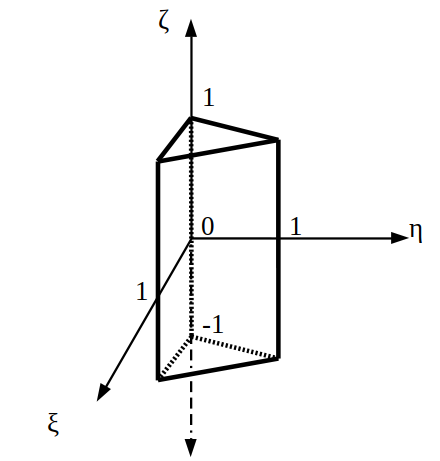
\includegraphics[width=0.3\textwidth]{Wref}
        \caption{Description of Reference Wedge.}
        \label{fig:Wref}
      \end{figure}

      The reference wedge $W_{ref}$ is located in 
      $\xi \in [0,1]$, $\eta \in [0,1-\xi]$, and $\zeta \in [-1,1]$. The
      coordinate system of the reference wedge is shown in \fref{fig:Wref}. The
      basis functions are zero outside of the reference wedge and are 
      provided within the reference wedge.
      \begin{align}
        \basis_i(\xi,\eta,\zeta) &= 0 \quad \forall \; (\xi,\eta,\zeta)
          \notin W_{ref} \\
        \basis_1(\xi,\eta,\zeta) &= \half (1-\zeta)(1-\xi-\eta) \\
        \basis_2(\xi,\eta,\zeta) &= \half (1-\zeta)\xi \\
        \basis_3(\xi,\eta,\zeta) &= \half (1-\zeta)\eta \\
        \basis_4(\xi,\eta,\zeta) &= \half (1+\zeta)(1-\xi-\eta) \\
        \basis_5(\xi,\eta,\zeta) &= \half (1+\zeta)\xi \\
        \basis_6(\xi,\eta,\zeta) &= \half (1+\zeta)\eta 
      \end{align}

      The integrals of the basis function over the element are given in
      \eref{eq:bigmat} through \eref{eq:wedge_surface_integral}. The values
      presented herein are not found in literature and have been calculated by
      the author. For a general wedge, the integral quantities are
      \begin{align}
        \label{eq:bigmat}
        \int_{\Omega_e} \basis_i(\vr) \basis_j(\vr) \;d\vr &= 
          \frac{V_e}{144}
          \begin{pmatrix}
            4 & 2 & 2 & 2 & 1 & 1 \\
            2 & 4 & 2 & 1 & 2 & 1 \\
            2 & 2 & 4 & 1 & 1 & 2 \\
            2 & 1 & 1 & 4 & 2 & 2 \\
            1 & 2 & 1 & 2 & 4 & 2 \\
            1 & 1 & 2 & 2 & 2 & 4 
          \end{pmatrix}, \\
        \int_{\Omega_e} \basis_i(\vr) \;d\vr &= \frac{V_e}{12}, \\
        \label{eq:wedge_surface_integral}
        \int_{\partial \Omega_e} \basis_i(\vr) 
          \basis_j(\vr) \;ds &= 
          \begin{cases}
            \frac{A_{\triangle}}{12}(1+\delta_{ij}) & 
              \text{if triangular surface,} \\
            \frac{A_{\Box}}{36}(1+\delta_{ij})(1-\half \delta_{i,(5-j)}) &
              \text{if quadrilateral surface,}
          \end{cases}
      \end{align}
      where $V_e$ is the volume of the element, $A_{\triangle}$ is the area of 
      the triangular surface, and $A_{\Box}$ is the area of the quadrilateral
      surface.  The matrix in \eref{eq:bigmat} is indexed $\mathbf{M}_{ij}$ and
      is presented as a matrix because of its irregular form. Notice the
      integral containing the gradient operator has been omitted because it is
      computed using a quadrature. If it could be computed analytically, it
      would be less computationally efficient than using a quadrature.
      
      $A_{\triangle}$ is computed according to \eref{eq:area_triangle} and
      $A_{\Box}$ is computed as the sum of the area of two triangles, employing
      the same formula. For a simple extruded triangle, the volume calculation 
      is straightforward and is the product of triangular area and linear 
      height. However, allowing the nodes to move with respect to each other 
      makes the volume of the element difficult to calculate. Therefore, the 
      Jacobian is used to calculate $V_e$. For more detail, see 
      \sref{sec:quadratures}, especially \tref{tab:jacobi}.

  \subsection{Quadratures}
    \label{sec:quadratures}
    Quadratures are sets of coordinates and weights which are used to
    approximate an integral.  For a given set of weights, $\{w_i\}$, and a set
    of coordinates, $\{\vx_i\}$, an integral can be represented as the sum
    \begin{equation}
      \label{eq:quadrature}
      \int_{\Omega} f(\vx) \;d\Omega \approx \sum_{i=1}^{N} f(\vx_i) \, w_i 
    \end{equation}
    where $\Omega$ is an arbitrary domain described by $\{\vx_i\}$.  A
    quadrature, such as the one in \eref{eq:quadrature}, can be designed to
    exactly integrate a polynomial of order $n$. It is not necessarily true that
    the number of quadrature points, $N$, will equal the order of the polynomial
    exactly integrated, $n$. Generally, $n \ne N$.
    
    For one-dimensional integrals, the Gaussian quadrature is common and the most compact quadrature. The Gaussian quadrature exactly integrates a 
    polynomial of order $n$ using exactly $N=n$ points. For this quadrature, the
    number of points in the quadrature is the same as the order of the
    quadrature and $n=N$.
    
    Two-dimensional and three-dimensional quadratures are necessary for the 
    \gls{fem}. Triangular quadratures are not as simple to derive
    as line quadratures and the number of points need not equal the order of the
    polynomial integrated. The triangular quadrature as implemented here is 
    symmetric and open. That is, there are no points on the boundary of the 
    triangle \cite{triangleQuadrature}. Any triangular quadrature will suffice
    that exactly integrates polynomials of a given order. There is no fixed
    relationship between $n$ and $N$ and for this quadrature, $n \ne N$.
    
    Quadrilateral quadrature sets are simply tensor products of two line 
    Gaussian quadratures. For an order $n$ polynomial, now $N^2=n$ points are 
    required. 
    
    Wedge quadrature sets are simply tensor products of a line Gaussian 
    quadrature and a triangular quadrature. Again, there is no fixed
    relationship between $n$ and $N$.
    
    Though only linear functions are used here, basis functions are generally
    polynomials of first, second, or third order; that is, linear, quadratic, or
    cubic functions. The quadratures described are capable of exactly
    integrating polynomial functions of given order so there exists a quadrature
    order that will exactly integrate the finite element quantities to numeric
    precision. The table of the order required for exact integration are
    provided in \tref{tab:quadrature_orders}.

    \begin{table}
      \begin{center}
        \caption{Quadrature Orders for \glsentryshort{fem} Quantities.}
        \label{tab:quadrature_orders}
        \begin{threeparttable}
          \begin{tabular*}{0.8\textwidth}{@{\extracolsep{\fill}}lccc}
            \toprule
            Quantity & Linear & Quadratic & Cubic \\
            \midrule
            $\int_{\Omega} \basis_i(\vr) \;d\Omega$ & 1 & 2 & 4
              \tnote{$\dagger$} \\
            $\int_{\Omega} \basis_i(\vr) \basis_j(\vr) \;d\Omega$ &
              2 & 4 & 6 \\
            $\int_{\Omega} \grad \basis_i(\vr) \cdot \grad \basis_j(\vr) 
              \;d\Omega$ & 2 & 3 & 5 \\
            \bottomrule
          \end{tabular*}
          \begin{tablenotes}
            \item[$\dagger$] A third-order quadrature would be exact but the 
              triangular quadrature would have negative weights so a fourth 
              order quadrature is selected.
          \end{tablenotes}
        \end{threeparttable}
      \end{center}
    \end{table}
    
    All of the quadratures described here are tabulated for a reference element
    be it a line, triangle, quadrilateral, or wedge. Integration in the 
    \gls{fem} is performed on an arbitrary element in space. Therefore, it is 
    necessary to perform a coordinate transform when using a quadrature set.
    % get VERY explicit here so someone else can actually solve the problem...
    Integration with transformed coordinates from domain $\Omega$ to the
    reference domain $\Omega_{ref}$ can be written
    \begin{equation}
      \int_{\Omega} f(\vx) \;d\Omega = 
        \int_{\Omega_{ref}} f(\vx) \lvert \mj \rvert \;d\Omega_{ref} \approx
        \sum_{i=1}^{N} w_i f(\vx_i) \lvert \mj_i \rvert
    \end{equation}
    where $\mj$ is the Jacobian matrix, $\mj_i$ is the Jacobian matrix at 
    quadrature coordinate $\vx_i$, and $\lvert \cdot \rvert$ represents
    the matrix determinant. Notationally, $J=\lvert \mj \rvert$ and is termed
    the Jacobi.

    Isoparametric elements are elements in which shape functions can be used to
    relate global coordinates, $(x,y,z)$, to local coordinates
    $(\xi,\zeta,\eta)$. Generally, non-curved elements are isoparametric. For
    isoparametric elements, such as triangles and wedges, the Jacobi is constant
    over the element and can be pre-calculated. Pre-calculating the Jacobi
    avoids populating and evaluating the determinant of a matrix for each
    integration point. For the elements of concern, these values are presented
    in \tref{tab:jacobi} \cite{textbookcolorado}.

    \begin{table}
      \caption{Jacobi for Selected Elements.}
      \label{tab:jacobi}
      \begin{center}
        \begin{tabular}{ll}
          \toprule
          Element & $J$ \\
          \midrule
          Triangle      & $A_e$ \\
          Quadrilateral & $\frac{1}{4} A_e$ \\
          Wedge         & $\half V_e$ \\
          \bottomrule
        \end{tabular}
      \end{center}
    \end{table}

    For the general element, the Jacobian matrix, $\mj_i$, is calculated at each
    point of the quadrature $(\xi_i,\zeta_i,\eta_i)$ as described in
    \eref{eq:calcJacobian}.
    \begin{equation}
      \label{eq:calcJacobian}
      \mj_i = 
      \begin{pmatrix}
        \sum_{k=1}^{N_P} \left. \frac{\partial \basis_k}{\partial \xi}
          \right|_{(\xi_i,\zeta_i,\eta_i)} x_k   \; &
        \sum_{k=1}^{N_P} \left. \frac{\partial \basis_k}{\partial \zeta}
          \right|_{(\xi_i,\zeta_i,\eta_i)} x_k   \; &
        \sum_{k=1}^{N_P} \left. \frac{\partial \basis_k}{\partial \eta} 
          \right|_{(\xi_i,\zeta_i,\eta_i)} x_k   \\
        \sum_{k=1}^{N_P} \left. \frac{\partial \basis_k}{\partial \xi}
          \right|_{(\xi_i,\zeta_i,\eta_i)} y_k   \; &
        \sum_{k=1}^{N_P} \left. \frac{\partial \basis_k}{\partial \zeta} 
          \right|_{(\xi_i,\zeta_i,\eta_i)} y_k   \; &
        \sum_{k=1}^{N_P} \left. \frac{\partial \basis_k}{\partial \eta} 
          \right|_{(\xi_i,\zeta_i,\eta_i)} y_k   \\
        \sum_{k=1}^{N_P} \left. \frac{\partial \basis_k}{\partial \xi}
          \right|_{(\xi_i,\zeta_i,\eta_i)} z_k   \; &
        \sum_{k=1}^{N_P} \left. \frac{\partial \basis_k}{\partial \zeta} 
          \right|_{(\xi_i,\zeta_i,\eta_i)} z_k   \; &
        \sum_{k=1}^{N_P} \left. \frac{\partial \basis_k}{\partial \eta} 
          \right|_{(\xi_i,\zeta_i,\eta_i)} z_k   
      \end{pmatrix}
    \end{equation}
    In \eref{eq:calcJacobian}, $N_P$ is the number of points in the element, 
    $\basis_k(\vr)$ is the basis function centered at the $k^{th}$ corner, and 
    for corner coordinates $(x_k,y_k,z_k)$ for $k = 1,2,\ldots,N_P$.

    With the Jacobian populated as \eref{eq:calcJacobian}, $J=\lvert\mj\rvert$
    is simply the matrix determinant. For the quadrature integration of 
    derivative quantities as necessary in the \gls{fem}, the derivatives must 
    also be translated from the reference element to the spatial element. This 
    is performed according to \algorithmref{algorithm:deriv_int}. The notation 
    is dense as the method requires two sets of coordinates. First, the 
    coordinate in the reference element $(\xi,\zeta,\eta)$ and second, the 
    coordinate in Cartesian space $(x,y,z)$.

    The vector $\vd_{i,\,(\xi,\zeta,\eta)}$ is the gradient vector for
    $\basis_i$ with respect to the reference coordinates $(\xi,\zeta,\eta)$.
    \begin{equation}
      \vd_{i\,(\xi,\zeta,\eta)} = \grad_{(\xi,\zeta,\eta)} N_i(\vr) 
    \end{equation}
    Vector $\vd_{i,\,(x,y,z)}$ is the gradient vector for $\basis_i$ with
    respect to the Cartesian coordinates $(x,y,z)$. 
    \begin{equation}
      \vd_{i,\,(x,y,z)} = \grad_{(x,y,z)} N_i(\vr)
    \end{equation}
    In \algorithmref{algorithm:deriv_int}, the quadrature has points $\{\vx_p\}$ 
    and weights $\{w_p\}$ for $p = 1,2,\ldots,N$ and the value of the integral,
    $v$, is represented by \eref{eq:deriv_integral}.
    \begin{equation}
      \label{eq:deriv_integral}
      v = \int_{\Omega_e} \grad_{(x,y,z)} \basis_i(\vr) \cdot 
        \grad_{(x,y,z)} \basis_j(\vr) \; d\Omega_e
    \end{equation}

    \begin{algorithm}
      \caption{Integral of Derivative with Jacobian Method.}
      \label{algorithm:deriv_int}
      \begin{algorithmic}[1]
        \State $v=0$
        \For{$p=1,N_P$}
          \State Calculate the Jacobian $\mj$ as in \eref{eq:calcJacobian}.
          \State Calculate the vector $\vd_{i,\,(\xi,\zeta,\eta)}$ at quadrature
            point $\vx_p$.
          \State Calculate the vector $\vd_{j,\,(\xi,\zeta,\eta)}$ at quadrature
            point $\vx_p$.
          \State Invert and store the Jacobian $\mj^{-1}$.
          \State Calculate the vector $\vd_{i,\,(x,y,z)} =
            \vd_{i,\,(\xi,\zeta,\eta)} \mj^{-1}$.
          \State Calculate the vector $\vd_{j,\,(x,y,z)} =
            \vd_{j,\,(\xi,\zeta,\eta)} \mj^{-1}$.
          \State $v = v + \left(\vd_{i,\,(x,y,z)}^{T} \vd_{j,\,(x,y,z)}\right)
            \, w_p \, \lvert \mj \rvert$
        \EndFor
      \end{algorithmic}
    \end{algorithm}

\section{Power Iterations}
  \label{sec:power_iterations}
  The \gls{fem} is used to solve a fixed source problem for a given source
  distribution $q_g(\vr)$. However, for multigroup problems with a fission
  source, the problem is an eigenvalue problem and the source is not known.
  For eigenvalue problems, the problem does not have a fixed source and the
  system has many solutions. The method of Power Iterations allows eigenvalue
  problems to be solved iteratively for the fundamental eigenvalue and
  eigenvector.

  \subsection{Convergence of Power Iteration Method}
    Noting the \gls{fem} equations can be written as matrix form
    \eref{eq:matrix_notation}, the discretized multigroup neutron diffusion 
    equation can be rewritten as shown by \textcite{gehinThesis} as
    \begin{equation}
      \label{eq:gehin_notation}
      \mb(\vPhi,\keff) \vPhi = \frac{1}{\keff} \mm \vPhi
    \end{equation}
    where $\vPhi$ is the vector of the flux containing all energy groups, matrix 
    $\mb$ contains the diffusion, removal, and all scattering terms, and $\mm$ 
    includes all fission generation and operates on $\vPhi$ and $\keff$. $\mb$
    is an S-matrix and its inverse, $\mb^{-1}$, exists and has all positive 
    elements \cite{nakamura}. Therefore, \eref{eq:gehin_notation} can be 
    rewritten as
    \begin{equation}
      \label{eq:gehin_solution}
      \vPhi = \frac{1}{\keff} \mr \vPhi
    \end{equation}
    where
    \begin{equation}
      \label{eq:gehin_r}
      \mr = \mb^{-1} \mm.
    \end{equation}
    Matrix $\mm$ is non-symmetric and is non-negative and $\mb$ is an S-matrix;
    therefore, $\mr$ is a non-symmetric, non-negative matrix.

    In the solution of \eref{eq:multigroup_diffusion}, the largest eigenvalue,
    $\keff$, is desired along with its associated eigenvalue, $\phi_g$. The
    solution can be found using the method of power iterations which can be
    written as 
    \begin{align}
      \label{eq:power_iteration_phi}
      \vPhi^{(s+1)} &= \frac{1}{\keff^{(s)}} \mr \vPhi^{(s)}, \\
      \label{eq:power_iteration_eigenvalue}
      \keff^{(s+1)} &= \keff^{(s)} \frac{\vw^{T} \vPhi^{(s+1)}}
        {\vw^{T} \vPhi^{(s)}}, \qquad s = 1,2,\ldots,\infty,
    \end{align}
    where $s$ is the iteration counter, $\vw$ is a weighting vector and 
    $\vw^{T} \vPhi$ is the vector inner-product. According to the 
    Perron-Frobenius theorem, a matrix with the properties of $\mr$ has a 
    unique, positive eigenvalue, greater in magnitude than the modulus of all 
    other eigenvalues of the matrix. The weighting vector $\vw$ is arbitrary 
    but does affect convergence rate. For this work,
    $\vw = \{\nu \Sigma_f\}$ such that the inner product 
    $\{\nu \Sigma_f\}^T \vPhi$ represents the summation of the fission neutron
    production rate throughout all energy groups and all elements. 
    
    It can then be shown in that the method of power iterations described in 
    \eref{eq:power_iteration_phi} and \eref{eq:power_iteration_eigenvalue}
    converges to the largest eigenvalue, $\keff$, and unique positive 
    eigenvector $\vPhi$ \cite{nakamura}. For notation and enumeration, allow the 
    eigenvalue to be rewritten as
    \begin{equation}
      \label{eq:mu}
      \mu = \frac{1}{\keff}.
    \end{equation}
    The eigenvectors $\vu_n$ and
    corresponding eigenvalues $\mu_n$ of $\mr$ are defined by
    \begin{equation}
      \label{eq:eigen_definition}
      \vu_n = \mu_n \, \mr \, \vu_n.
    \end{equation}
    It may be proved that all eigenvalues $\mu$ are real, positive, and 
    distinct. The eigenvalues are then numbered in the sequence
    \begin{equation}
      \label{eq:eigen_order}
      \mu_0 < \mu_1 < \mu_2 < \cdots < \mu_N
    \end{equation}
    where $N$ is the rank of the problem. The eigenvectors have the 
    orthogonality relations
    \begin{equation}
      \label{eq:eigen_orthogonality}
      \vu^T_n \vu_m = 0  \qquad \text{for } n \ne m
    \end{equation}
    where $\vu^T \vu$ is the vector inner-product. Assume eigenvectors are
    normalized such that
    \begin{equation}
      \label{eq:eigen_normalization}
      \vu_n^T \vu_n = 1 \qquad \text{for } n = 1, 2, \ldots, N.
    \end{equation}
    The initial vector $\vPhi^{(0)}$ may be expressed as a projection onto the
    eigenvectors using a linear superposition of eigenvectors of the form
    \begin{equation}
      \label{eq:eigen_projection}
      \vPhi^{(0)} = \sum_{n=1}^{N} c_n^{(0)} \vu_n
    \end{equation}
    where $c_n^{(0)}$ is a coefficient given by the orthogonality relationship
    from \eref{eq:eigen_orthogonality} such that
    \begin{equation}
      \label{eq:eigen_cn}
      c_n^{(0)} = \vu_n^T \vPhi^{(0)}.
    \end{equation}
    Using this eigenmode projection, \eref{eq:power_iteration_phi} can be
    rewritten as 
    \begin{equation}
      \label{eq:phi_expand_begin}
      \vPhi^{(s+1)} = \mu^{(s)} \, \mu^{(s-1)} \, \mu^{(s-2)} \, 
        \ldots \, \mu^{(0)} \, \mr \phi^{(0)}.
    \end{equation}
    Then, \eref{eq:eigen_projection} can be inserted into
    \eref{eq:phi_expand_begin}.
    \begin{align}
      \vPhi^{(s+1)} &= \mu^{(s)} \, \mu^{(s-1)} \, \ldots \, 
        \mu^{(0)} \sum_{n=1}^N c_n^{(0)} \, \mr \, \vu_n \\
      &= \left( \prod_{p=0}^{s} \mu^{(p)} \right) \sum_{n=1}^N c_n^{(0)} \, 
        \mr \, \vu_n
    \end{align}
    Recalling the relationship \eref{eq:eigen_projection}.
    \begin{equation}
      \label{eq:phi_expand_above}
      \vPhi^{(s+1)} = \left( \prod_{p=0}^s \mu^{(p)} \right) 
        \sum_{n=1}^N c_n^{(0)} \frac{1}{\mu_n^{(s+1)}} \vu_n
    \end{equation}
    \eref{eq:phi_expand_above} can be rewritten by dividing and multiplying by
    $\mu_0$ and dividing and multiplying by $c_0$.
    \begin{align}
      \vPhi^{(s+1)} &= \left( \prod_{p=0}^s \frac{\mu^{(p)}}{\mu_0} 
        \right) c_0 \left( \vu_0 \sum_n^N \frac{c_n^{(0)}}{c_0^{(0)}}
        \frac{\mu_0}{\mu_n^{(s+1)}} \vu_n \right) \\
      \label{eq:eigen_phi_converge}
      \vPhi^{(s+1)} &\approx \text{const.} \cdot \left( 
        \vu_0 \sum_n^N \frac{c_n^{(0)}}{c_0^{(0)}}
        \frac{\mu_0}{\mu_n^{(s+1)}} \vu_n \right)
    \end{align}
    The ordering of unique eigenvalues required by \eref{eq:eigen_order} 
    requires $\mu_0 / \mu_n < 1$ and the problem is convergent. The 
    convergence rate is determined by the dominance ratio, $d$, where
    \begin{equation}
      \label{eq:dominance_ratio}
      d \equiv \max_{n=1,2,\ldots,N} \frac{\mu_0}{\mu_n} =
        \frac{\mu_0}{\mu_1}
    \end{equation}
    and it can be seen that for problems with small dominance ratio, the power
    iteration method will converge more quickly. As the dominance ratio
    approaches unity, $d \rightarrow 1$, the power iteration method will be
    slower to converge. Convergence criteria are then specified as an absolute 
    tolerance in the sense of the eigenvalue
    \begin{equation}
      \label{eq:eigenvalue_tol}
      \epsilon_{\mu} > | \mu^{(s+1)} - \mu^{(s)} |
    \end{equation}
    and as a relative tolerance in the sense of the eigenvector
    \begin{equation}
      \label{eq:eigenvector_tol}
      \epsilon_{\vPhi} > \max_i \left| \frac{\vPhi_i^{(s+1)} - \vPhi_i^{(s)}}
        {\vPhi_i^{(s)}}\right| .
    \end{equation}

    It is important to note that all of the analysis in this section assumed the
    matrix $\mr$ does not change between iterations. For simple multigroup
    criticality calculations, this assumption is correct. However, in
    multiphysics nuclear power reactor simulations, the cross sections of the 
    problem may be considered functions of material temperature or may have some
    variable number density. For these problems, the matrix $\mr$ is necessarily
    updated between power iterations in a nonlinear manner. For nonlinear power
    iteration updates, convergence is no longer guaranteed. The argument for
    convergence with nonlinear power iterations in this implementation falls
    back to the stability of the physical system.
    
  \subsection{Calculation of Source with Power Iterations}
  \label{sec:calculation_of_source_with_power_iterations}
    The multigroup neutron diffusion equation \eref{eq:multigroup_source} can be
    written with the source term $q_g(\vr)$ expanded into its component parts.
    \begin{equation} \label{eq:multigroup_source_expand}
      -\grad \cdot (D_g(\vr) \grad \phi_g^{(s)}(\vr)) + \Sigma_{r,g}(\vr)
      \phi_g^{(s)}(\vr) = q_{fiss,g}(\vr) + q_{up,g}(\vr) + q_{down,g}(\vr)
    \end{equation}
    Recall from the definitions of the source components that their calculation
    requires the flux $\phi_g(\vr)$. The source components each require
    different energy groups of the flux distribution to be known. The fission
    component $q_{fiss,g}(\vr)$ requires all groups. The up-scatter component
    $q_{up,g}(\vr)$ requires lower energy groups (i.e. $g' > g$). The
    down-scatter component $q_{down,g}(\vr)$ requires higher energy groups (i.e.
    $g' < g$). Based on these requirements, these source components can be
    calculated based on different iterations within the power iteration method.
    This is described in \algorithmref{algorithm:general}.
    \eref{eq:multigroup_source_expand} is then more explicitly written.
    \begin{equation} 
      \label{eq:multigroup_power_iterations}
      -\grad \cdot (D_g(\vr) \grad \phi_g^{(s+1)}(\vr)) + \Sigma_{r,g}(\vr)
      \phi_g^{(s+1)}(\vr) = q_{fiss,g}^{(s)}(\vr) + q_{up,g}^{(s)}(\vr) +
      q_{down,g}^{(s+1)}(\vr)
    \end{equation}

\section{Implementation}
  A \gls{fem} neutron diffusion solution has been developed using 
  the above formulae. The program begins by reading a geometry description 
  specified in a plain text VTK file \cite{vtk}. The VTK format is chosen 
  because it is a standard that can be used with visualization tools such as 
  ParaView \cite{ParaView} and VisIt \cite{VisIt}. Additionally, open-source C 
  and Python packages exist for easy manipulation of the format. Cross sections
  are specified in either a plain text user format or the ISOTXS format as 
  common to fast reactor applications and the multigroup cross section generator
  \mcc \cite{mcc}. The multigroup neutron diffusion equation is solved according
  to \eref{eq:multigroup_source}. The resulting effective neutron multiplication 
  factor, $\keff$, is written to an output file. The multigroup neutron flux is
  written to a different results VTK file for easy visualization. In a
  multiphysics simulation, material temperatures and thermal expansion
  dimensions are also written to the results VTK.

  \subsection{Algorithm}
    The algorithm for the solution to the diffusion equation is similar to most
    implementations of the power iteration method to solve the multigroup
    neutron diffusion equation. The algorithm itself is presented in 
    \algorithmref{algorithm:general}. The steps unique to the \gls{fem} are 
    steps \ref{state:fem_matrix} and \ref{state:fem_vector}. These require the 
    quantities previously derived and form the linear system described by the 
    \gls{fem}. 

    In step \ref{state:rcm} the matrix is reordered. Mathematically this has no
    effect on the result as the linear system represented is equivalent. This 
    choice to reorder the system is made to improve computational efficiency. 
    Indexing nodes that are physically proximate with proximate indices causes 
    rows in the finite element matrix, $\ma_g$, to be closely coupled to nearby
    rows. In a general unstructured and unordered mesh, rows may be coupled to 
    other random rows in the matrix. This step of reordering the matrix $\ma_g$ 
    seeks to decrease the bandwidth of the matrix and encourage cache hits when
    accessing coupled values in the linear system. The ordering chosen is the
    \gls{rcm} method and common to sparse linear systems
    \cite{rcm}. An example of the bandwidth reduction provided by the \gls{rcm}
    method is shown in \fref{fig:sparsity_pattern}. The plots show the
    sparsity pattern of the matrix before and after reordering. After
    reordering, the matrix bandwidth is reduced from 2,326 to 81.

    \begin{figure}
      \centering
      \subfloat{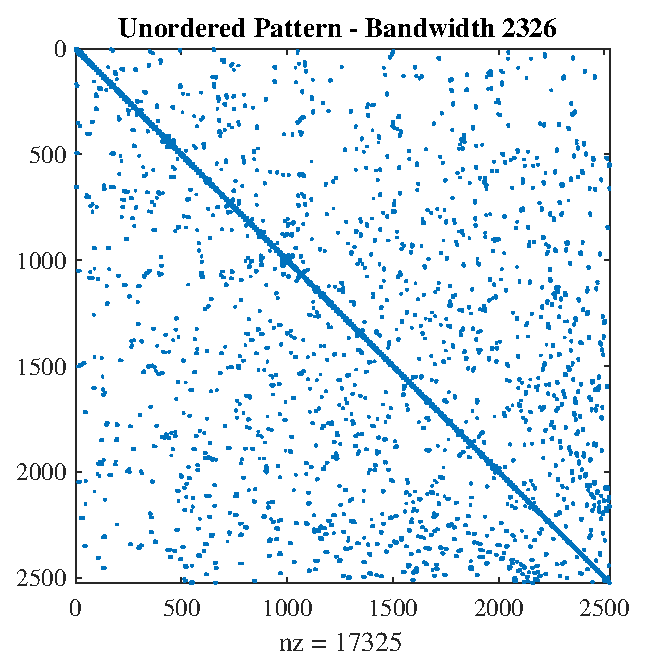
\includegraphics[width=0.4\textwidth]{uno_pattern}}
      \hspace{0.1in}
      \subfloat{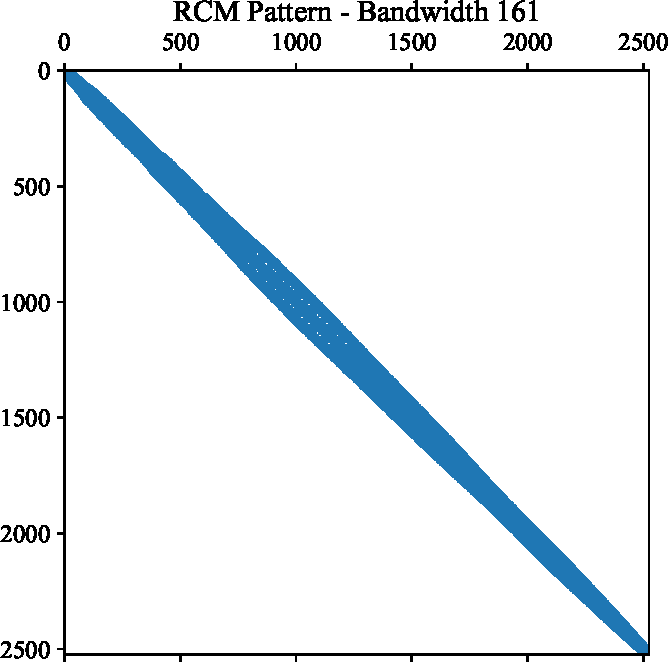
\includegraphics[width=0.4\textwidth]{rcm_pattern}}
      \caption{Demonstration of \glsentryshort{rcm} Matrix Ordering.}
      \label{fig:sparsity_pattern}
    \end{figure}
    
    \begin{algorithm}
      \caption{General Iteration Scheme}
      \label{algorithm:general}
      \begin{algorithmic}[1]
      \State Read mesh from VTK.
      \State Initialize $\phiavg_g^{(0)}$.
      \State Order the nodes of the mesh into \gls{rcm} order.
        \label{state:rcm}
      \State Calculate $\Sigma_{s,g'\rightarrow g}$, $\Sigma_{r,g}$, and 
        $\nu \Sigma_{f,g}$ for each element.
      \State Calculate finite element matrix $\ma_g$ for each group. Store this. 
        \label{state:fem_matrix}
      \While{Power Iteration}
        \State Update the iteration counter. $s=s+1$
        \State Update $q_{fiss,g}$ and $q_{up,g}$ for all groups from previous 
          data $\phiavg^{(s-1)}$.
        \State Update $\widetilde{\chi_g}$ in each element using previous data.
          \label{state:chi_collapse}
        \For{$g=1,G$}
          \State Update $q_{down,g}$ from current data $\phiavg_g^{(s)}$
          \State Calculate total source in each element.
          \State Update finite element Vector $\vf_g$ with new source.
            \label{state:fem_vector}
          \State Solve $\ma_g \vu_g = \vf_g$ using an iterative technique (See
            \sref{sec:linear_system_solution}).
          \State Parse $\vu_g$ for $\phi_g$ solution on nodes.
          \State Calculate element-average $\phiavg_g$.
        \EndFor
        \State Update $\keff$.
        \State Check convergence.
        \State Perform non-linear update if necessary and update $\ma_g$. 
          \label{state:nonlinear}
      \EndWhile
      \end{algorithmic}
    \end{algorithm}

    Step \ref{state:nonlinear} in \algorithmref{algorithm:general} incorporates
    the possibility of non-linear updates into the power iteration method. This
    invalidates the proof of convergence from \sref{sec:power_iterations} but is
    performed to simulate thermal hydraulic and thermal expansion effects as
    described in \chref{ch:thermalHydraulics} and \chref{ch:thermalExpansion}
    respectively. This procedure is commonly used in practice and no convergence 
    problems have been observed. This update also requires recalculating the 
    finite element matrix, $\ma_g$, for each group.
    
    A benefit of this implementation is that the finite element vector $\vf_g$
    must be updated on each power iteration of the solution whereas the matrix
    $\ma_g$ is described entirely by geometry and the material cross sections.
    For this reason, in problems with no multiphysics simulations, $\ma_g$ can
    be generated once at the beginning of the problem and stored for the
    duration of the calculation.

    \FloatBarrier % make sure the algorithm is in the correct section

  \subsection{Memory and Storage}
    The finite element matrix, $\ma_g$, is large and sparse so a sparse storage 
    and sparse solution to the linear system are required. Many sparse matrix 
    implementations have been described and implemented in the past including
    triplet, reduced column, and reduced row storage \cite{sparseBLAS}.  For 
    this work a \twotable method is chosen which was uniquely developed. 
    \twotable storage is chosen for its simplicity and implementation with the 
    \gls{fem}. Future work may include a reduced row implementation but there 
    will be a trade-off between memory minimization and computational 
    efficiency.
    
    The \twotable method is composed of two separate matrices in memory. An
    integer index table, \texttt{IDX}, and an IEEE double precision value table
    \texttt{VAL}. Table \texttt{IDX} is is dimension $DOF \times D$ where $DOF$
    is the number of degrees of freedom of the linear system and $D$ is the
    maximum number of nodes that a node shares including itself. $D$ is the
    degree of the matrix plus one. This must be determined at the beginning of
    the problem based on the input geometry.  Table \texttt{VAL} is dimension
    $DOF \times D \times G$ where $G$ is the number of energy groups as the
    matrix $\ma_g$ is group dependent.
    
    \texttt{IDX} is initialized to -1 and \texttt{VAL} is initialized 
    to 0.0 such that an index of -1 corresponds to a null entry in the 
    matrix. \texttt{IDX} is then populated with a modified adjacency graph. 
    Values in \texttt{IDX} indicate the column in which the \texttt{VAL} entry
    occurs. An example unstructured mesh is given in \fref{fig:adjacency_graph}. 
    Then, for node 5, the table \texttt{IDX} may resemble \eref{eq:idx_example}.
    \begin{equation}
      \label{eq:idx_example}
      \texttt{IDX}(:,5) = (8, 200, 48, 96, 5 )
    \end{equation}

    \begin{figure}
      \centering
      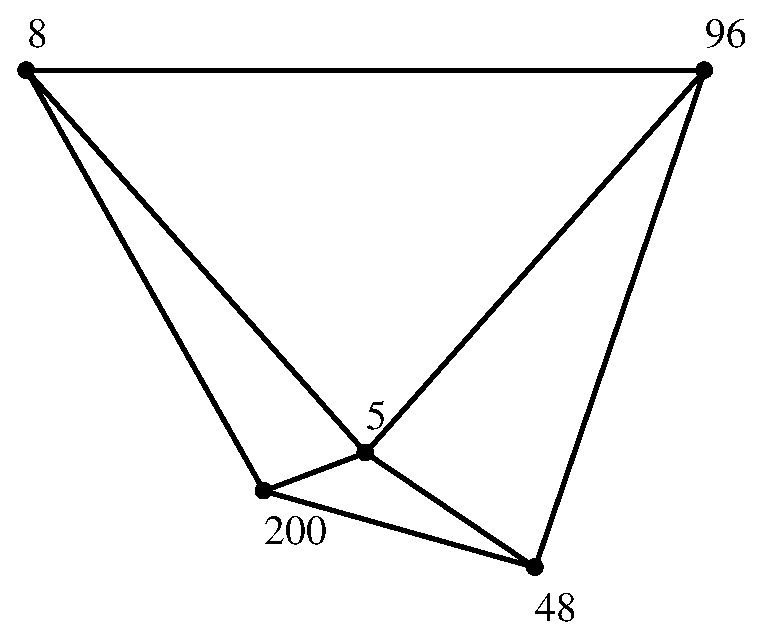
\includegraphics[width=0.5\textwidth]{adjacency_graph}
      \caption{Example Unstructured Mesh.}
      \label{fig:adjacency_graph}
    \end{figure}

    \eref{eq:idx_example} is only an example because the order of the nodes in 
    row 5 is arbitrary. Similarly, a numeric example is provided in 
    \eref{eq:idx_number} (note that the value ``3'' is arbitrary).
    \begin{equation}
      \label{eq:idx_number}
      \left.
      \begin{array}{c}
        \texttt{IDX}(7,3) = 8 \\
        \texttt{VAL}(7,3,g) = 12.1
      \end{array}
      \right\}
      \implies
      A_{7,8,g} = 12.1
    \end{equation}
    \eref{eq:idx_number} indicates that the value of matrix $\ma_g$ for group
    $g$ in the seventh row in the eighth column is 12.1. This will allow for 
    simple row operations and efficient matrix-vector multiplication which will
    be necessary in the solution of the linear system.

  \subsection{Boundary Conditions}
    \label{sec:boundary_conditions}
    Boundary conditions merit brief consideration. There are many ways to 
    implement boundary conditions and all result in mathematically the same 
    solution. The choices made for this work are presented below. Mirror 
    boundary conditions require $\grad \phi_g(\vr) = 0$ for 
    $\vr \in \partial \Omega$. These are termed ``natural'' boundary
    conditions because the finite element matrix, $\ma_g$, requires no
    additional treatment and this condition is natural. In the albedo
    representation, this is equivalent to $\albedo = 0$.
    
    Albedo boundary conditions are treated with an additional contribution to 
    the finite element matrix, $\ma_g$. These contributions represent a line 
    integral in two dimensions and a surface integral in three dimensions. These
    values are found in \eref{eq:matrix_population} and the quantities are 
    expressed in \sref{sec:matrix_quantities} or by quadratures 
    \sref{sec:quadratures}.
    
    Zero-flux boundary conditions require $\phi_g(\vr) = 0$ for $\vr \in
    \partial \Omega$. These are treated by removing these entries from the
    finite element matrix, $\ma_g$. Entries are removed by using an index vector.
    In a problem with only mirror and albedo boundary conditions, each node
    corresponds to an index row/column of the matrix. With entries removed, node
    number and index number may not exactly agree. A vector \texttt{ID} is
    introduced to track node numbers and their location in the finite element
    matrix, $\ma_g$ \cite{textbookjohnson}. Nodes with non-zero flux boundary
    conditions are set to a sequential positive integer. Nodes with zero-flux
    boundary conditions are set to a negative integer (-1) and are omitted in
    the actual solution of the system. Other strategies have been proposed such
    as the penalty approach \cite{textbookhughes} and forcing the solution of
    the linear system \cite{textbookli}. This method is chosen because it
    decreases the degree of freedom of the linear system while encouraging a
    well conditioned matrix.  Now, the degree of freedom of the matrix is equal
    to the number of nodes with non-zero flux boundary conditions.
    Alternatively, zero-flux boundary conditions can be represented as $\albedo
    \rightarrow \infty$.
    
  \subsection{Linear System Solution}
    \label{sec:linear_system_solution}
    For a non-singular linear system $\ma_g \vu_g = \vf_g$, where $\ma_g$ is a 
    square matrix, there exists a unique solution. Many strategies have been 
    proposed to solve this system in an efficient manner. Options are restricted
    in this work because the solution must operate with a sparsely stored linear
    system and result in no fill-in. This immediately demands an iterative
    method. The linear system described by the \gls{fem} can then be exploited
    for its unique properties to select a favorable solution method.
    
    The finite element matrix $\ma_g$ for the problem described in
    \eref{eq:multigroup_source} is \gls{spd} if the multigroup equations are
    solved one group at a time as they are in this work. Note, the matrix will 
    not have this especially useful property if all the groups were instead
    solved simultaneously. The symmetry condition is straight-forward and is
    observed in the elemental matrix description \eref{eq:matrix_population}.
    Briefly, $\ma_g^T = \ma_g$ because the elements ${A_{i,j,g,e}=A_{j,i,g,e}}$.
    Positive definiteness is a particularly useful condition but is often
    difficult to prove. $\ma_g$ is sometimes diagonally dominant for
    conveniently ordered meshes composed certain elements but generally, the
    matrix is not diagonally dominant. 
    
    A matrix $\ma_h \in \realnn$ is positive definite if
    \begin{equation} \label{eq:positive_definite}
      \vx^{T} \ma_g \vx > 0 \qquad \forall \; \vx \in \realn, \; \vx \ne 0.
    \end{equation}
    Let $\vx = \{x_i\}$ for $i = 1,2,\ldots,N$. Then the vector-matrix and 
    matrix-vector products can be rewritten as summations \cite{textbookhughes}.
    \begin{equation}
      \vx^{T} \ma_g \vx = \sum_{i=1}^{N} \sum_{j=1}^{N} x_i A_{ij} x_j
    \end{equation}
    By the definition of $A_{i,j,g}$ in \eref{eq:matrix_population} and 
    \eref{eq:fem_notation}.
    \begin{equation}
      \vx^{T} \ma_g \vx = 
        \sum_{i=1}^{N} \sum_{j=1}^{N} x_i a_g(\basis_i,\basis_j) x_j
    \end{equation}
    Noting the property that $a_g(\cdot,\cdot)$ is a bilinear operator (i.e.
    linear in both arguments) \cite{textbookli}.
    \begin{equation}
      \vx^{T} \ma_g \vx =
        a_g \left( \sum_{i=1}^{N} x_i \basis_i, \sum_{j=1}^{N} x_j \basis_j 
        \right)
    \end{equation}
    By construction of the \gls{fem}, $w(\vr) = \sum_{i=1}^{N} x_i \basis_i$ 
    where $w(\vr)$ is a piecewise continuous polynomial of arbitrary order.
    \begin{equation}
      \vx^{T} \ma \vx = a_g \left(w(\vr),w(\vr)\right)
    \end{equation}
    $a(\cdot,\cdot)$ can be shown to form a norm $\|\cdot \|_a$
    \cite{textbookli} satisfying the positive definite condition
    \eref{eq:positive_definite}.
    \begin{equation}
      \vx^{T} \ma_g \vx > 0 \qquad \forall \vx \in \realn, \; \vx \ne 0
    \end{equation}
    
    A given matrix can be verified as positive definite by one of two methods.
    First, all eigenvalues of the matrix have positive real components. Second,
    the matrix has a Cholesky decomposition such that $\ma = \ml \, \ml^*$ where
    $\ml$ is a lower triangular matrix with positive diagonal entries and
    $\ml^*$ is the conjugate transpose of matrix $\ml$ \cite{textbookipsen}. For
    real valued matrices, the conjugate transpose is equivalent to the
    conventional transpose. Though an eigenvalue decompisition or a Cholesky
    factorization may be useful for debugging or numerical analysis purposes, 
    these operations are computationally expensive. Instead, this is verified 
    here for the general matrix and not tested during simulations.
    
    Conventional methods used to solve a linear system described by an \gls{spd}
    matrix include Gauss-Seidel iteration with \gls{sor} and the \gls{cg} Krylov 
    subspace method. \gls{sor} requires \textit{a priori} knowledge of the 
    optimized over-relaxation factor, $\omega_{opt}$, for optimal performance. 
    In practice, calculation of $\omega_{opt}$ is performed analytically for 
    contrived solutions or in a modified guess-and-check method. The \gls{cg} 
    method is chosen because it requires no \textit{a priori} knowledge and
    produced a solution to the same tolerance in a reduced wall-time without the
    need for guess-and-check iterations.
    
    A simple recipe for the \gls{cg} method is replicated in
    \algorithmref{algorithm:CG} \cite{Kelley1995IterativeEquations}.
    
    \begin{algorithm}
      \caption{\glsentrylong{cg} Method.}
      \label{algorithm:CG}
      \begin{algorithmic}[1]
        \State $k = 0$
        \State $\vr = \vb - \ma \vx$
        \State $\rho_k = \|\vr\|_2^2$
        \State $k = k + 1$
        \While{$\sqrt{\rho_{k-1}} > \epsilon \|\vb\|_2$}
          \If{$k=1$}
            \State $\vp = \vr$
          \Else
            \State $\beta = \rho_{k-1} / \rho{k-2}$
            \State $\vp = \vr + \beta \vp$
          \EndIf
          \State $\vw = \ma \vp$
          \State $\beta = \rho_{k-1} / \vp^{T} \vw$
          \State $\vx = \vx + \beta \vp$
          \State $\vr = \vr - \beta \vw$
          \State $\rho_k = \| \vr \|_2^2$
          \State $k=k+1$
        \EndWhile
      \end{algorithmic}
    \end{algorithm}
    
    In \algorithmref{algorithm:CG}, $\epsilon$ is a tolerance set by the user 
    and the square of the two-norm is most efficiently replaced by the vector
    inner-product as in \eref{eq:two_norm_inner}. 
    \begin{equation}
      \label{eq:two_norm_inner}
      \|\vr\|_2^2 = \vr^{T} \vr
    \end{equation}
    It is noted that this method requires minimal storage with only four vectors 
    required ($\vx, \vw, \vp,$ and $\vr$). Additionally, each iteration requries
    only two scalar products and a single matrix-vector product which proves to
    be the most computationally expensive \cite{Kelley1995IterativeEquations}.
    As most of the computational time of the diffusion solutions is spent in the
    linear system solution, is is crucial that this process be efficient.

    With the solution of the linear system, the implementation of the \gls{fem}
    to solve the multigroup neutron diffusion problem is completed. Results in 
    the form of analytic and benchmark verification problems are presented in
    \chref{ch:diffusionResults}.

\chapter{THERMAL HYDRAULICS}
\label{ch:thermalHydraulics}

\section{Axial Convection Model}
\section{Radial Conduction Model}
  \subsection{Derivation}
  \subsection{Relations}
\section{Cross Section Treatment}
\section{Results}

\chapter{THERMAL EXPANSION}
\label{ch:thermalExpansion}

\section{Necessity of Modeling}
  % discuss the EBR-II tests

\section{Model Details}

\section{Implementation}

\section{Results}

\chapter{CONCLUSIONS}
\label{ch:conclusions}

\section{Results Discussion}
\section{Code Enhancements}
\section{Further Investigations}

%\restoregeometry


%%---------------------------------------------------------------------------%%
%%  Bibliography 
%\ensureoddstart
\begin{spacing}{1}
 \setlength\bibitemsep{11pt} %22pt = 2*11pt, where fontsize is 11pt
 \phantomsection
 %\textorpdfstring and \uppercase needed due to hyperref package 
 % http://www.latex-community.org/forum/viewtopic.php?f=44&t=16601
 \addcontentsline{toc}{chapter}{\bibname}
 %\vspace{-0.5in}
\titleformat{\chapter}[display]{\bf\filcenter
}{\chaptertitlename\ \thechapter}{11pt}{\bf\filcenter}
\titlespacing*{\chapter}{0pt}{-0.5in-9pt}{22pt}

\printbibliography[heading=myheading]
\end{spacing}
%\bibliographystyle{apalike}

%%---------------------------------------------------------------------------%%
% Appendices
%\ensureoddstart
\restoregeometry
\appendix
\newgeometry{margin=1in,lmargin=1.25in,footskip=\chapterfootskip, includehead,
  includefoot}

\chapter{Analytic Solutions to the Neutron Diffusion Equation}
\label{ap:analyticSolutions}

\section{Introduction}
  The following is a manufactured solution designed for verification of one,
  two, and three-dimension numerical neutron diffusion equation solvers.
  one-group and two-group problems are also addressed.
  
  For the reference problems, the one-group neutron diffusion problem is written
  below.
  \begin{equation} \label{eq:onegroup}
    -D \grad^2 \phi + \Sigma_r \phi =  \frac{1}{\keff} \nu \Sigma_f \phi + 
      q_{fixed}
  \end{equation}
  Where $\grad^2 \phi = \grad \cdot (\grad \phi)$ and is used to simplify 
  notaiton. For two-group neutron diffusion problems, the two-group neutron 
  diffusion problem is written below.
  \begin{align} 
    \label{eq:twogroup1}
    -D_1 \grad^2 \phi_1 + \Sigma_{r1} \phi_1 &= \frac{1}{\keff} \left(
      \nu \Sigma_{f1} \phi_1 + \nu \Sigma_{f2} \phi_2 \right) \\
    \label{eq:twogroup2}
    -D_2 \grad^2 \phi_2 + \Sigma_{r2} \phi_2 &= 
      \Sigma_{s 1 \rightarrow 2} \phi_2
  \end{align}
  Where $\phi_1$ is the higher energy group and $\phi_2$ is the lower energy 
  group. This formulation assumes all fission neutrons are created in the fast 
  energy group and there is no up-scattering (scattering that results in an 
  increase in neutron energy). These are realistic assumptions for all diffusive
  neutron systems.

  Analytic solutions are provided herein. One-dimension problems can be 
  replicated in a two-dimension solver using a square geometry and select 
  boundary conditions. For a given quadrilateral, two of the boundary conditions
  are set to reflective conditions and two are set to zero-flux $(\phi = 0)$ 
  conditions. For true two-dimensions problems, all of the boundary conditions 
  are set to zero-flux conditions.
  
  These formula are common to second order partial differential equations but
  the formulation here is based in part from \cite{textbooklewis}.

\section{One-Dimension, One-Group, Fixed Source}
  \label{sec:deriv_1dfixedsrc}
  This one-dimension problem is in the domain $x \in [0,L]$. For this problem, 
  the following one-group coefficients are used.
  \begin{align*}
    D &= 1\\
    \Sigma_r &= 1\\
    \nu \Sigma_f &= 0\\
    q_{fixed} &= 1
  \end{align*}
  Then, \eref{eq:onegroup} is written
  \begin{equation} \label{eq:fixed_source}
    - \grad^2 \phi(x) + \phi(x) = 1 
  \end{equation}
  \eref{eq:fixed_source} can also be rewritten.
  \begin{equation} \label{eq:diffusion_simplified}
    \grad^2 \phi(x) - B^2 \phi(x) = S
  \end{equation}
  where $B = 1$ and $S=-1$.
  The solution is composed of a particular and general solution.
  \begin{equation}
    \phi(x) = \phi_g(x) + \phi_p(x)
  \end{equation}
  For problems of the form of \eref{eq:diffusion_simplified} the general 
  solution has exponential or hyperbolic trigonometric form.
  \begin{equation} \label{eq:fixedsource_general}
    \phi_g(x) = c_1 \cosh(Bx) + c_2 \sinh(Bx)
  \end{equation}
  Where $c_1$ and $c_2$ are problem dependent constants. For $S=1$ as constant
  in the problem domain, the particular solution has given form.
  \begin{align} \label{eq:particular}
    \phi_p(x) &= -S/B \\
           &= 1
  \end{align}
  Then, the combined solution has the given form.
  \begin{equation} 
    \phi(x) = c_1 \cosh(Bx) + c_2 \sinh(Bx) + 1
  \end{equation}
  The only remaining step is to solve for constants $c_1$ and $c_2$. These are
  zero-flux boundary conditions at the problem boundaries.
  \begin{align}
    \label{eq:bcx0}
    \phi(0) &= 0\\
    \label{eq:bcxL}
    \phi(L) &= 0
  \end{align}
  Evaluating the solution at 0, 
  \begin{align}
    \phi(0) &= 0 \\
    &= c_1 + 1\\
    c_1 &= -1
  \end{align}
  Evaluating the solution at $L$
  \begin{align}
    \phi(L) &= 0\\
    &= c_2 \sinh(BL) - \cosh(BL)-1\\
    c_2 &= \frac{\cosh(BL)-1}{\sinh(BL)}
  \end{align}
  The final solution is 
  \begin{equation} \label{eq:analytic_1dfixedsrc}
    \phi(x) = -\cosh(Bx) + \frac{\cosh(BL)-1}{\sinh(BL)} \sinh(Bx) +1
  \end{equation}
  
\section{One-Dimension, One-Group, Criticality} 
  \label{sec:deriv_1d1g}
  This one-dimension problem is in the domain $x \in [0,L]$.
  This problem also uses the one-group neutron diffusion equation from 
  \eref{eq:onegroup}. For this problem, and the following coefficients:
  \begin{align*}
    D &= 1\\
    \Sigma_r &= 1\\
    \nu \Sigma_f &= 2\\
    q_{fixed} &= 0
  \end{align*}
  The problem is then proposed as 
  \begin{equation}
    -\grad^2 \phi(x) - \phi(x) = 0 
  \end{equation}
  and has general solution
  \begin{equation} \label{eq:critical_general}
    \phi_g(x) = c_1 \cos(x) + c_2 \sin(x)
  \end{equation}
  Considering zero-flux boundary conditions from \eref{eq:bcx0} and 
  \eref{eq:bcxL}, then $c_1 = 0 $ yielding
  \begin{equation} \label{eq:sinshape}
    \phi_g(x) = c_2 \sin(x)
  \end{equation}
  The problem is an eigenvalue problem and has infinite solutions so the 
  constant $c_2$ is arbitrary for $\sin(x)=0$. Introducing a Buckling term $B$
  then $B=\frac{n \pi}{L}$ and $\sin(Bx)=0$ for $n$ an odd integer. The 
  fundamental mode is then $B=\frac{1}{L}$. Therefore, the solution is 
  \begin{equation} \label{eq:analytic_1d1g}
    \phi(x) = \sin(x/L)
  \end{equation}
  Inserting this solution back into \eref{eq:onegroup} and dividing both sides
  by $\sin(x/L)$ will yield an expression for $\keff$.
  \begin{align}
    -D B^2 + \Sigma_r &= \frac{1}{\keff} \nu \Sigma_f \\
    \keff &= \frac{\nu \Sigma_f}{DB^2 + \Sigma_r} \label{eq:keff1d}
  \end{align}
  Then, for a slab of length $ L = 100 \units{cm} $, $B = \pi / 100$ and
  \begin{equation}
    \keff = 1.9980280254
  \end{equation}
  
\section{Two-Dimension, One-Group, Criticality}
  \label{sec:deriv_2d1g}
  The same material coefficients are used for this problem as in the 
  one-dimension, criticality problem. For this problem, the domain is in the 
  rectangle $[0,L_x]\times[0,L_y]$. Similar to the one-dimension problem, 
  this problem has basic solution of $\sin(x/L)$. The problem is separable in 
  the two spatial dimensions. 
  \begin{equation}
    \phi(x,y) = X(x) Y(y) 
  \end{equation}
  Beginning with equation \eref{eq:onegroup}.
  \begin{align}
    -D \grad^2 \phi(x,y) + \Sigma_r \phi(x,y) &= \nu \Sigma_f \phi(x,y) \\
    - \grad^2 \phi(x,y) - \phi(x,y) &= 0 \\
    \grad^2 \phi(x,y) + \phi(x,y) &= 0 \\
    \frac{\partial^2}{\partial x^2} \phi(x,y) + 
      \frac{\partial^2}{\partial y^2} \phi(x,y) +
      \phi(x,y) &= 0\\
    Y(y)\frac{\partial^2}{\partial x^2}X(x) +
      X(x) \frac{\partial^2}{\partial y^2} Y(y) + X(x)Y(y) &= 0\\
    Y(y)\left(\frac{\partial^2}{\partial x^2}X(x) + \frac{1}{2} X(x)\right)+
      X(x)\left(\frac{\partial^2}{\partial y^2}Y(y) + \frac{1}{2}Y(y)
      \right) &= 0
  \end{align}
  For non-trivial solutions $X(x) \ne 0$ and $Y(y) \ne 0$ then the following
  second order ordinary differential equations can be solved.
  \begin{align}
    \frac{d^2}{dx^2} X(x) + \frac{1}{2} X(x) &= 0 \\
    \frac{d^2}{dy^2} Y(y) + \frac{1}{2} Y(y) &= 0 \\
  \end{align}
  The solution to these problems is the product of the solutions from the 
  previous problem presented in \eref{eq:analytic_1d1g}. The solution is
  \begin{equation} \label{eq:analytic_2d1g}
    \phi(x,y) = \sin(x/A) \sin(y/B)
  \end{equation}
  Where $L_x$ is the horizontal extent of the rectangular domain and $L_y$ is 
  the vertical extent of the rectangular domain. Extending the concept of 
  geometric buckling to the two spatial dimensions where $B_x = \frac{1}{L_x}$
  and $B_y = \frac{1}{L_y}$. If $B=B_x=B_y$; that is, $L_x=L_y$, $\keff$ can 
  be calculated as
  \begin{equation}
    \keff = \frac{\nu \Sigma_f}{2DB^2 + \Sigma_r} 
  \end{equation}
  Then, for $A=B = 100 \units{cm}$
  \begin{equation}
    \keff = 1.9960599356
  \end{equation}
  
\section{One-Dimension, Two-Group, Criticality}
  \label{sec:deriv_1d2g}
  Much of this section is drawn from course notes prepared by Dr. Scott 
  Palmtag \cite{analytic2g}.
  
  A two-group neutron diffusion problem is considered for a one-dimension
  homogeneous slab in the domain $x \in [0,L]$. Energy group 1 is higher energy
  than energy group 2. It is assumed all fission neutrons are  produced in the
  fast group (i.e. $\chi_1=1$ and $\chi_2=0$). Additionally, it is assumed that 
  there is no up-scattering  (i.e. $\Sigma_{2\rightarrow1}=0$).  Then, the
  two-group neutron diffusion equations are given in \eref{eq:twogroup1} and 
  \eref{eq:twogroup2}.
  
  Referring to the problem posed by Section \sref{sec:deriv_1d1g}, the flux 
  solutions have form given in equation \eref{eq:sinshape}. Then
  \begin{align}
    \label{eq:twogroupflux1}
    \phi_1(x) &= c_1 \sin(Bx) \\
    \label{eq:twogroupflux2}
    \phi_2(x) &= c_2 \sin(Bx)
  \end{align}
  Where $B$ is the geometric buckling term. For this geometry, the geometric 
  buckling of the fundamental mode is given by 
  \begin{equation}
    B = \pi/L_x
  \end{equation}
  Then, inserting \eref{eq:twogroupflux1} and \eref{eq:twogroupflux2} into 
  \eref{eq:twogroup2} and dividing the equation by $\sin(Bx)$
  \begin{equation}
    D_2 B^2 c_2 + \Sigma_{r2} c_2 = \Sigma{s1\rightarrow2} c_1
  \end{equation}
  Then, the ratio can be expressed
  \begin{equation} \label{eq:fluxratio}
    \frac{c_2}{c_1} = \frac{\Sigma_{s1\rightarrow2}}{D_2 B^2 + \Sigma_{r2}}
  \end{equation}
  The ratio $\frac{c_2}{c_1}$ represents the relative magnitude of thermal to 
  fast flux. Returning to \eref{eq:twogroup1}, and using in 
  \eref{eq:twogroupflux1} and \eref{eq:twogroupflux2} and again dividing both
  sides by  $\sin(Bx)$
  \begin{align}
    D_1 B^2 c_1 &= \frac{1}{\keff} \left( \nu \Sigma_{f1} c_1 + 
      \nu \Sigma_{f2} c_2\right)\\
    \keff &= \frac{\nu \Sigma_{f1} c_1 + \nu \Sigma_{f2} c_2}
      {D_1 B^2 c_1 + \Sigma{r1} c_1}\\
    \keff &= \frac{\nu \Sigma_{f1} + \nu \Sigma_{f2} c_2/c_1}
      {D_1 B^2 + \Sigma{r1}}
  \end{align}
  Inserting the expression from \eref{eq:fluxratio}
  \begin{equation}
    \keff = \frac{\nu \Sigma_{f1} + \nu \Sigma_{f2} 
      \left(\frac{\Sigma_{s1\rightarrow2}}{D_2B^2+\Sigma_{r2}}\right)}
      {D_1 B^2 + \Sigma{r1}}
  \end{equation}
  From the VVER-440 benchmark \sref{sec:vver440}, material 1,
  \begin{align*}
    D_1 &= 1.3466  \\
    D_2 &= 0.37169 \\
    \Sigma_{r1} &= 2.5255\text{E}-2\\
    \Sigma_{r2} &= 6.4277\text{E}-2\\
    \nu \Sigma_{f1}  &= 4.4488\text{E}-3\\
    \nu \Sigma_{f2}  &= 7.3753\text{E}-2\\
    \Sigma_{s1\rightarrow2} &= 1.6893\text{E}-2 \\
    k_{\infty} &= 0.943664259
  \end{align*}
  For a 100 \units{cm} slab.
  \begin{align}
    \frac{c_2}{c_1} &= 0.26132419 \\
    \keff &= 0.892349025
  \end{align}
  
\section{One-Dimension, One-Group, Two Region, Criticality}
  \label{sec:deriv_2reg}
  This final analytic problem was designed to test the materials mapping of a
  solver. The problem is proposed as a slab reactor with a fuel and reflector
  region. The neutron diffusion equation is given in  \eref{eq:onegroup}. 
  Geometry is described in \fref{fig:2reg_geom}. Fuel Material (subscript F) 
  is located in $x \in [0,a]$ and Reflector Material (subscript R) is located in
  $x \in [a,b]$.
  \begin{figure}
    \centering
    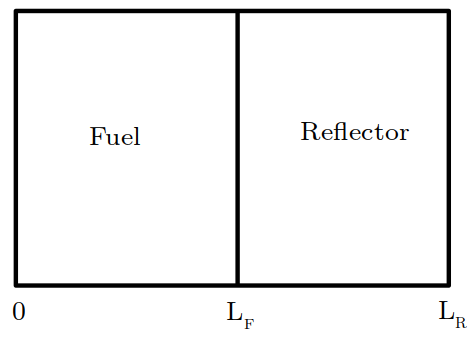
\includegraphics[width=0.6\textwidth]{2reg_geom}
    \caption{Geometry for Two Region Problem.}
    \label{fig:2reg_geom}
  \end{figure}
  Boundary conditions on the horizontal surfaces (top/bottom) are reflective
  to reduce the problem to one-dimension. Other boundary conditions are given
  below. Noting $\phi'(x) = \frac{d \phi}{dx}$.
  \begin{align}
    \label{eq:2reg_mirror}
    \phi'_F(0)&=0\\
    \label{eq:2reg_continuity}
    D_F\phi'_F(a)&=D_R\phi'_R(a) \\
    \label{eq:2reg_fluxcontinuity}
    \phi_F(a) &= \phi_R(a) \\
    \label{eq:2reg_zeroflux}
    \phi_R(b)&=0
  \end{align}
  These represent mirror condition at $x=0$, current continuity at $x=a$, flux
  continuity at $x=a$, and zero-flux at $x=b$. The material properties are 
  specified in \tref{tab:2reg_constants}.
  \begin{table}
    \caption{Two Region Material Constants.}
    \label{tab:2reg_constants}
    \begin{center}
      \begin{tabular}{crr}
        \toprule
        & Fuel & Reflector \\
        \midrule
        $D$ & 1.2 & 0.7 \\
        $\Sigma_r$ & 0.02 & 0.015 \\
        $\nu \Sigma_f$ & 0.02 & 0 \\
        $q_{fixed}$ & 0 & 0 \\
        \bottomrule
      \end{tabular}
    \end{center}
  \end{table}
  
  The general form of the solution in the fueled region has form similar to 
  \eref{eq:critical_general}.
  \begin{equation}
    \phi_F(x) = c_{1F} \cos(B_F x) + c_{2F} \sin(B_F x)
  \end{equation}
  Then, using the mirror boundary condition at $x=0$ \eref{eq:2reg_mirror}.
  \begin{align}
    \phi_F(x) &= c_{1F} \cos(B_F x) + c_{2F} \sin(B_F x) \\
    \phi'_F(x) &= -B_F c_{1F} \sin(B_F x) + B_F c_{2F} \cos(B_F x) \\
    \phi'_F(0) &= 0\\
    &=B_F c_{2F}
  \end{align}
  Therefore, $c_{2F}=0$ and
  \begin{equation}
    \phi_F(x) = c_{1F} \cos(B_F x)
  \end{equation}
  Because this is an eigenvalue problem, $c_{1F}$ is arbitrary and $B_F$ 
  represents the buckling factor in the Fuel Material.
  
  Now for the solution in the reflector region. The solution has general form
  similar to \eref{eq:fixedsource_general}.
  \begin{equation}
    \phi_R(x) = c_{1R} \cosh(B_R (x-a)) + c_{2R} \sinh(B_R (x-a))
  \end{equation}
  The coordinate transform $(x-a)$ is equivalent to multiplying by a constant 
  because $\sinh$ and $\cosh$ can be rewritten as exponentials and due to 
  exponential properties. Treating the zero-flux boundary condition at $x=b$ 
  \eref{eq:2reg_zeroflux}.
  \begin{align}
    \phi_R(x) &= c_{1R} \cosh(B_R (x-a)) + c_{2R} \sinh(B_R (x-a))\\
    \phi_R(b) &= 0 \\
    &= c_{1R} \cosh(B_R(b-a)) + c_{2R} \sinh(B_R(b-a))\\
    c_{1R} &= -c_{2R} \frac{\sinh(B_R(b-a))}{\cosh(B_R(b-a))}\\
    c_{1R} &= -c_{2R} \tanh(B_R(b-a))\\
    c_{2R} &= -c_{1R} \frac{1}{\tanh(B_R(b-a))} \label{eq:c2rnumber1}
  \end{align}
  Treating the current continuity boundary condition at $x=a$ 
  \eref{eq:2reg_continuity}.
  \begin{align}
    D_F \phi'_F(a) &= D_R \phi'_R(a) \\
    -D_F c_{1F} B_F \sin(B_F a) &= D_R B_R c_{2R} \\
    c_{2R} &= -\frac{D_F c_{1F} B_F \sin(B_F a)}{D_R B_R} \label{eq:c2rnumber2}
  \end{align}
  Treating the flux continuity boundary condition at $x=a$ 
  \eref{eq:2reg_fluxcontinuity}.
  \begin{align}
    \phi_F(a)&=\phi_R(a) \\
    c_{1F} \cos(B_F a) &= c_{1R} \\
    c_{1R} &= c_{1F} \cos(B_F a) \label{eq:c1r}
  \end{align}
  Setting equations \eref{eq:c2rnumber1} and \eref{eq:c2rnumber2} equal.
  \begin{equation}
    - \frac{D_F c_{1F} B_F \sin(B_F a)}{D_R B_R} = -c_{1R} \tanh(B_R(b-a))
  \end{equation}
  Using the the expression for $c_{1R}$ from \eref{eq:c1r}
  \begin{align}
    - \frac{D_F c_{1F} B_F \sin(B_F a)}{D_R B_R} &=
      - \frac{c_{1F} \cos(B_F a)}{\tanh(B_R(b-a))}\\
    \frac{D_F B_F \sin(B_F a)}{D_R B_R} &= 
      \frac{\cos(B_F a)}{\tanh(B_R(b-a))} \\
    B_F \tan(B_F a) &= \frac{D_R B_R}{D_F \tanh(B_R(b-a))}
  \end{align}
  By material definition,  ${B_R = \sqrt{\Sigma_{rR}/D_R}}$.
  
  This is the most simplified solution. Unfortunately, there is no analytic
  expression for $B_F$. Therefore, a numeric solver must be used such as 
  MATLAB's \texttt{vpasolve()} or a generic bisection/binary search. The $\tan()$ 
  function causes the solution to $B_F$ is especially sensitive to the starting
  guess.
  
  Once $B_F$ is known, the problem is solved.
  \begin{align}
    \phi_F(x) &= \phi_0 \cos(B_F x)\\
    \phi_R(x) &= \phi_0 \cos(B_F a) \cosh(B_R (x-a)) 
      - \frac{D_F \phi_0 \sin(B_F a)}{D_R B_R} \sinh(B_R (x-a))\\
    \label{eq:analytic_2reg}
    \phi(x) &= H(x-a)\phi_R(x) + H(a-x)\phi_F(x)
  \end{align}
  Where $H(x)$ is the Heaviside step function.  
  
  The eigenvalue for this problem can be expressed for a known $B_F$. Similar 
  to \eref{eq:keff1d}. In this problem, for $a=50 \units{cm}$ and
  $b=100 \units{cm}$ and material constants given in \tref{tab:2reg_constants}.
  \begin{align}
    B_F &= 0.0255922048213879 \\
    \keff &= \frac{\nu\Sigma_{fF}}{D_F B_F^2 + \Sigma_{rF}} \\
    &= 0.9621882561
  \end{align}
\section{Finite-Cylinder, One-Group, Criticality}
  \label{sec:deriv_finite_cyl}
  The finite cylinder is an example of a truly three-dimension problem with
  an analytic solution. This is a homogeneous cylinder with zero-flux boundary
  conditions on the edge of the cylinder. The cylinder has height $H$ and 
  radius $T$. The coordinates $r\in[0,T]$ and $z\in[0,H]$ where 
  $r=\sqrt{x^2+y^2}$.
  
  The solution method is by separation of variables into radial and axial 
  directions. This derivation is similar to that in \sref{sec:deriv_2d1g}.
  Beginning with the one-group neutron diffusion equation \eref{eq:onegroup} 
  and assuming that  $\phi(r,z) = R(r) Z(z)$.
  \begin{align}
    -D \grad^2 \phi(r,z) + \Sigma_r \phi(r,z) &= \nu \Sigma_f \phi(r,z) \\
    \grad^2 \phi(r,z) + \frac{\nu\Sigma_f - \Sigma_r}{D} \phi(r,g) &= 0 \\
    \frac{1}{r} \frac{\partial}{\partial r} \left( r \frac{\partial}{\partial r}
      \phi(r,z) \right) + \frac{\partial^2}{\partial z^2} \phi(r,z) +
      \frac{\nu\Sigma_f - \Sigma_r}{D} \phi(r,z) &= 0 \\
    Z(z) \frac{1}{r} \frac{\partial}{\partial r} \left( r 
      \frac{\partial}{\partial r} R(r) \right) + 
      R(r) \frac{\partial^2}{\partial z^2} Z(z) + 
      \frac{\nu\Sigma_f - \Sigma_r}{D} R(r) Z(z) &= 0 \\
    Z(z) \frac{1}{r} \frac{\partial}{\partial r} \left( r 
      \frac{\partial}{\partial r} R(r) \right) + 
      R(r) \frac{\partial^2}{\partial z^2} Z(z) + 
      B^2 R(r) Z(z) &= 0 \\
    Z(z) \left( \frac{1}{r} \frac{\partial}{\partial r} \left( r 
      \frac{\partial}{\partial r} R(r) \right) + \frac{B^2}{2} R(r) \right) + 
      R(r) \left( \frac{\partial^2}{\partial z^2} Z(z) + \frac{B^2}{2} Z(z) 
      \right) &= 0
  \end{align}
  For non-trivial solutions $R(r) \ne 0$ and $Z(z) \ne 0$ then the following
  second order ordinary differential equations can be solved.
  \begin{align}
    \label{eq:cyl_radialR}
    \frac{1}{r} \frac{\partial}{\partial r} \left( r \frac{\partial}{\partial r}
      R(r) \right) + \frac{B^2}{2} R(r) &= 0 \\
    \label{eq:cyl_axialZ}
    \frac{\partial^2}{\partial z^2} Z(z) + \frac{B^2}{2} Z(z) &= 0
  \end{align}
  
  Beginning with the axial direction. The diffusion equation can be rewritten as 
  \eref{eq:cyl_axialZ}.
  \begin{equation} \label{eq:simplediffusion}
    \grad^2 Z(z) + B_z^2 Z(z) = 0
  \end{equation}
  and has solution of the form \eref{eq:critical_general}.
  \begin{equation} \label{eq:cyl_axial}
    Z(z) = c_1 \cos(B_z z) + c_2 \sin(B_z z)
  \end{equation}
  Requiring zero-flux boundary conditions $\phi(0)=\phi(H)=0$ yields $c_1=0$. 
  Then $c_2$ is arbitrary and the buckling condition is $B_zH=\pi$ and $B_z=\pi/H$.
  
  Moving on to the radial direction. The diffusion equation can be written as
  \eref{eq:cyl_radialR}.
  \begin{equation}
    \grad^2 R(r) + B_r^2 R(r) = 0
  \end{equation}
  Noting the radial coordinates.
  \begin{align}
    \frac{1}{r} \frac{\partial}{\partial r} \left( r \frac{\partial R}
      {\partial r} \right) + B_r^2 R &= 0 \\
    \frac{\partial}{\partial r} \left( r \frac{\partial R}{\partial r}
      \right) + B_r^2 R &= 0
  \end{align}
  Noting the product rule of differentiation.
  \begin{align}
    r \frac{\partial^2 R}{\partial r^2} + \frac{\partial R}
      {\partial r} + B_r^2 r R &= 0 \\
    \frac{\partial^2 \phi}{\partial r^2} + \frac{1}{r} \frac{\partial R}
      {\partial r} + B_r^2 R &= 0 \label{eq:besselequation}
  \end{align}
  Noting equation \eref{eq:besselequation}, \cite{textbooklewis} Appendix B
  shows the equation has solution of the form
  \begin{equation} \label{eq:cyl_radial}
    R(r) = c_3 J_0(B_r r) + c_4 Y_0(B_r r)
  \end{equation}
  Where $J_0$ is the Bessel function of the first kind, zeroth order and $Y_0$
  is the Bessel function of the second kind, zeroth order. Requiring the flux
  to be finite at $r=0$ requires $c_4=0$ as 
  $\lim_{r\rightarrow0} Y_0(r) \rightarrow -\infty$. As this is an eigenvalue
  problem, $c_3$ is arbitrary. Zero flux boundary conditions requires 
  $B_r R=\alpha_0$ where $\alpha_0$ is the first root of the $J_0$ function and 
  $\alpha_0 \approx 2.4048$. Then $B_r=\alpha_0/R$.
  
  Combining the radial expression \eref{eq:cyl_radial} and the axial 
  expression \eref{eq:cyl_axial} yields the final expression for the flux.
  \begin{align} \label{eq:analytic_finite_cyl}
    \phi(r,z) &= J_0(B_r r) \sin(B_z z) \\
    &= J_0(r \alpha_0 / R) \sin(z \pi / H)
  \end{align}
  Inserting \eref{eq:analytic_finite_cyl} into the diffusion equation will yield 
  the buckling/criticality condition.
  \begin{equation}
    -D \left( \frac{1}{r} \frac{\partial}{\partial r} \left( r 
      \frac{\partial \phi}{\partial r} \right) + \frac{\partial^2 \phi}
      {\partial z^2} \right) + \Sigma_r \phi = \frac{1}{\keff} \nu 
      \Sigma_f \phi
  \end{equation}
  Beginning with the differentiation terms for simplicity. Axial 
  differentiation is straight-forward and presented below.
  \begin{equation}
    \label{eq:above}
    \frac{\partial^2 \phi}{\partial z^2} = -B_z^2 J_0(B_r r) \sin(B_z z)
  \end{equation}
  Radial differentiation must account for the radial geometry and is more 
  complex. First, note the following derivative relationship of the zeroth
  order Bessel function.
  \begin{equation} \label{eq:deriv_bessel0}
    \frac{d}{dr} J_0(\alpha r) = - \alpha J_1(\alpha r)
  \end{equation}
  And applying \eref{eq:deriv_bessel0} to \eref{eq:above}
  \begin{align}
    \frac{\partial \phi}{\partial r} &= -B_r \sin(B_z z) J_1(B_r r) \\
    r \frac{\partial \phi}{\partial r} &= -B_r \sin(B_z z) r J_1 (B_r r) 
  \end{align}
  Note the additional derivative relation for the general Bessel function.
  \begin{equation} \label{eq:deriv_besseln}
    \frac{d}{dr} J_n(r) = \frac{1}{2} \left( J_{n-1}(r) - J_{n+1}(r)\right)
  \end{equation}
  Evaluating the rest of the cylindrical derivative using
  \eref{eq:deriv_besseln} and the product rule.
  \begin{align}
    \frac{\partial}{\partial r} \left( r \frac{\partial \phi}{\partial r}
      \right) &= -B_r \sin(B_z z) \left(J_1(B_r r) + \frac{1}{2} B_r r \left(
      J_0(B_r r) - J_2(B_r r) \right) \right) \\
    \frac{1}{r} \frac{\partial}{\partial r} \left(r 
      \frac{\partial \phi}{\partial r} \right) &=
      -B_r \sin(B_z z) \left(\frac{1}{r} J_1(B_r r) + \frac{1}{2} B_r \left(
      J_0(B_r r) - J_2(B_r r) \right) \right)
  \end{align}
  Finally, inserting the expression for the Laplacian of the flux back into the
  diffusion equation.
  \begin{multline}
    D \left( B_r \sin(B_z z) \left( \frac{1}{r} J_1(B_r r) + \frac{1}{2} B_r
    \left( J_0(B_r r) - J_2(B_r r) \right) \right) + B_z^2 J_0(B_r r) \sin(B_z
    z) \right) + \Sigma_r J_0(B_r r) \sin(B_z z) = \\
    \frac{1}{\keff} \nu \Sigma_f J_0(B_r r) \sin(B_z z)
  \end{multline}
  Dividing through by $\sin(B_z z)$.
  \begin{multline}
    D \left( B_r \left( \frac{1}{r} J_1(B_r r) + \frac{1}{2} B_r
    \left( J_0(B_r r) - J_2(B_r r) \right) \right) + B_z^2 J_0(B_r r) \right)+
    \Sigma_r J_0(B_r r) = 
    \\\frac{1}{\keff} \nu \Sigma_f J_0(B_r r) 
  \end{multline}
  Dividing through by $J_0(B_r r)$ and expanding some terms.
  \begin{align}
    D \left( B_r \left( \frac{1}{r} \frac{J_1(B_r r)}{J_0(B_r r)} + 
      \frac{1}{2} \left(B_r - \frac{J_2(B_r r)}{J_0(B_r r)} \right) \right) 
      + B_z^2 \right)+ \Sigma_r &= \frac{1}{\keff} \nu \Sigma_f \\
    D \left( \frac{1}{r} B_r \frac{J_1(B_r r)}{J_0(B_r r)} + \frac{B_r^2}{2} -
      \frac{B_r^2}{2} \frac{J_2(B_r r)}{J_0(B_r r)} + B_z^2 \right) + \Sigma_r&=
      \frac{1}{\keff} \nu \Sigma_f  \\
    \frac{1}{r} B_r \frac{J_1(B_r r)}{J_0(B_r r)} + \frac{B_r^2}{2} -
      \frac{B_r^2}{2} \frac{J_2(B_r r)}{J_0(B_r r)} + B_z^2 + 
      \frac{\Sigma_r}{D} &= \frac{1}{\keff} \frac{\nu \Sigma_f}{D}\\
    \frac{1}{J_0(B_r r)} \frac{B_r^2}{2} \left(\frac{1}{r} \frac{2}{B_r} 
      J_1(B_r r) - J_2(B_r r) \right) + \frac{B_r^2}{2} + B_z^2 + 
      \frac{\Sigma_r}{D} &= \frac{1}{\keff} \frac{\nu \Sigma_f}{D}
  \end{align}
  Note the Bessel function recursion relationship.
  \begin{equation} \label{eq:bessel_recursion}
    J_{n+1}(\alpha r) + J_{n-1}(\alpha r) = \frac{2n}{\alpha r} J_n(\alpha r)
  \end{equation}
  Using \eref{eq:bessel_recursion} the term above is simplified.
  \begin{align}
    \frac{1}{J_0(B_r r)} \frac{B_r^2}{2} \left( J_0(B_r r) \right) + 
      \frac{B_r^2}{2} + B_z^2 + \Sigma_r &= \frac{1}{\keff} 
      \frac{\nu \Sigma_f}{D} \\
    B_r^2 + B_z^2 + \frac{\Sigma_r}{D} &= \frac{1}{\keff} \frac{\nu \Sigma_f}
      {D}
  \end{align}
  Now, an expression for the eigenvalue can be written.
  \begin{align}
    \keff &= \frac{\nu \Sigma_f}{D(B_r^2 + B_z^2) + \Sigma_r} \\
    &= \frac{\nu \Sigma_f}{D\left(\left(\frac{\alpha_0}{R}\right)^2 + 
      \left(\frac{\pi}{H}\right)^2 \right) + \Sigma_r} \\
    &= 0.996710620898177
  \end{align}
  NOTE: the shape of the boundary is extremely important for this  problem.
  Therefore, the mesh must be regenerated with a halved mesh parameter  $h$ for
  each refinement, rather than simply splitting nodes as splitting nodes would 
  not improve the description of the boundary.


\chapter{Brief Compendium of Neutron Diffusion Benchmarks}
\label{ap:benchmarks}

\section{Introduction}
  This appendix includes a description of several benchmark reactor problems.
  These include two-dimensional and three-dimensional reactor benchmark
  problems. These benchmark descriptions are not original works but
  replications of data obtained from other sources. The intent is to make the
  data more easily accessible for others solving similar problems. The
  benchmarks presented in this appendix are summarized in the case matrix in
  \tref{tab:benchmark_case_matrix}. The benchmarks presented in this appendix
  include two-dimensional and three-dimensional geometries as well as a variety
  of energy group structures.

  \begin{table}
    \caption{Case Matrix for Benchmark Solutions.}
    \label{tab:benchmark_case_matrix}
    \begin{center}
      \begin{tabular}{lccccc}
        \toprule
        Benchmark & Dimensions & Groups & Reactor Type &
          \parbox[t]{0.6in}{\centering Neutron \\ Spectrum} \\
        \midrule
        VVER440 & 2 & 2 & \glsentryshort{lwr} & Thermal \\
        SNR     & 2 & 4 & \glsentryshort{sfr} & Fast \\
        \glsentryshort{hwr}     & 2 & 2 & \glsentryshort{hwr} & Thermal \\
        IAEA ($\times4$)    & 2 & 2 & \glsentryshort{pwr} & Thermal \\
        MONJU   & 3 & 3 & \glsentryshort{sfr} & Fast \\
        KNK     & 3 & 4 & \glsentryshort{sfr} & Fast \\
        \bottomrule
      \end{tabular}
    \end{center}
  \end{table}

  All reactors in this section are based on a hexagonal design common to fast
  reactors. However, not all benchmarks presented are fast reactors. These
  benchmarks were used to perform solution verification for the neutron
  diffusion equation solution method in \chref{ch:neutronDiffusion}. As such,
  the cross sections presented are those necessary to solve the multigroup
  neutron diffusion equation. 

  \FloatBarrier

  For each benchmark problem, geometry and cross sections are presented. The 
  notation for cross sections are common to the field and noted below.
  \begin{conditions} % custom environment designed for this purpose
    $D_g$    & diffusion coefficient for energy group $g$ \units{cm}, \\
    $\Sigma_{r,g}$ & macroscopic removal cross section for energy group $g$ \units{$\frac{1}{\text{cm}}$}, \\
    $\nu \Sigma_{f,g}$ & number of fission neutrons times macroscopic fission cross section in energy group $g$ \units{$\frac{1}{\text{cm}}$}, \\
    $\Sigma_{s,g' \rightarrow g}$ & macroscopic scatter cross section from energy group $g'$ to energy group $g$ \units{$\frac{1}{\text{cm}}$}, \\
    $\chi_g$ & effective fission spectrum for energy group $g$,\\
    $\kref$ & effective neutron multiplication factor.
  \end{conditions}
  \noindent
  A reference $\kref$ is presented for each benchmark to the precision of the
  solution. When available, reference power distributions are presented. Note
  that the reference solutions presented are not analytic or exact solutions.
  The solutions presented in this appendix are are provided from other sources. 
  The precision of the reference depends on the source.

\section{Two-Dimensional Benchmark Problems}
  The two-dimensional benchmarks presented represent various energy group
  structures, geometries, assembly sizes, and boundary conditions. By varying
  these parameters, the combination of these benchmarks constitutes a rigorous
  testing suite that can be used for solution verification of general multigroup
  neutron diffusion solvers.
  
  \subsection{VVER440}
    \label{sec:vver440}
    This benchmark is presented with solution by \textcite{chao}.
    The problem is one-twelfth of a VVER-440 reactor with seven control rods
    inserted. There are 25 assemblies across the core diameter. The last ring of
    assemblies at the core periphery are non-fissile reflector assemblies as
    shown in \fref{fig:vver440_geom}. Each assembly has a flat-to-flat
    measurement of ${14.70~\units{cm}}$. Vacuum boundary condition ($\albedo =
    0.5$) is applied on the core periphery and all other boundaries are mirror
    boundary conditions ($\grad \phi_g \cdot \nhat = 0$). To the precision of
    the benchmark, the effective neutron multiplication factor is $\kref =
    1.00970$. Two-group cross sections for the problem are given in
    \tref{tab:vver440xs}. The fission spectrum is given in
    \tref{tab:vver440chi}. Assembly powers are given in \fref{fig:vver440_geom}.

    \begin{figure}
      \centering
      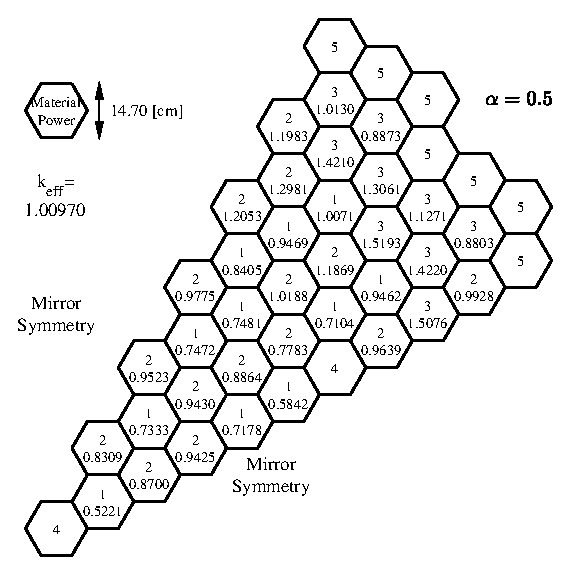
\includegraphics[width=0.7\textwidth]{vver440}
      \caption{VVER440 Geometry.}
      \label{fig:vver440_geom}
    \end{figure}

    \begin{table}
      \caption{VVER440 Cross Sections.}
      \label{tab:vver440xs}
      \begin{center}
        \begin{tabular}{cccccc}
          \toprule
          &MAT1&MAT2&MAT3&MAT4&MAT5\\
          \midrule
          $D_1$&1.346600E+00&1.337700E+00&1.332200E+00&1.195300E+00&1.448500E+00\\
          $D_2$&3.716900E-01&3.691800E-01&3.650200E-01&1.931300E-01&2.517600E-01\\
          $\Sigma_{r1}$&2.525500E-02&2.470900E-02&2.435000E-02&3.563600E-02&3.318400E-02\\
          $\Sigma_{r2}$&6.427700E-02&7.936100E-02&1.001000E-01&1.349800E-01&3.283900E-02\\
          $\Sigma_{s 1\rightarrow 2}$&1.689300E-02&1.591200E-02&1.488800E-02&2.226400E-02&3.226200E-02\\
          $ \nu \Sigma_{f1}$&4.448800E-03&5.533700E-03&7.039100E-03&&\\
          $ \nu \Sigma_{f2}$&7.375300E-02&1.058100E-01&1.496400E-01&&\\
          \bottomrule
        \end{tabular}
      \end{center}
    \end{table}

    \begin{table}
      \caption{VVER440 Fission Spectrum.}
      \label{tab:vver440chi}
      \begin{center}
        \begin{tabular}{cc}
          \toprule
          &Fission Spectrum \\
          \midrule
          $\chi_1$ & 1.0 \\
          $\chi_2$ & 0.0 \\
          \bottomrule
        \end{tabular}
      \end{center}
    \end{table}

  \subsection{SNR}
    \label{sec:snr}
    This benchmark is presented with solution in the Argonne Code Center
    Benchmark Problem Book \cite{argonneBenchmark}. It is based on the MARK-I
    core design of the SNR-300. The problem is one-sixth of a reactor with no
    control rods inserted. There are 17 assemblies across the core diameter with
    the outer rings being blanket assemblies as shown in \fref{fig:snr_geom}.
    Each assembly has a flat-to-flat measurement of ${11.20~\units{cm}}$. Vacuum
    boundary condition ($\albedo = 0.5$) is applied on the core periphery and
    all other boundaries are mirror boundary conditions ($\grad \phi_g \cdot
    \nhat = 0$). To the precision of the benchmark, the effective neutron
    multiplication factor is $\kref = 1.124$. Four-group cross sections for the
    problem are given in \tref{tab:snrxs}. The fission spectrum is given in
    \tref{tab:snrchi}. Assembly powers are not provided in the benchmark but can
    be calculated from existing codes (e.g. \dif).

    \begin{figure}
      \centering
      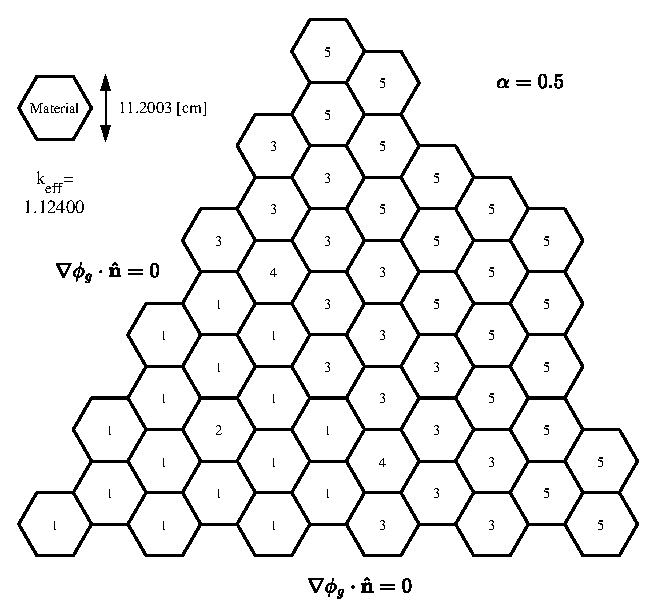
\includegraphics[width=0.7\textwidth]{snr}
      \caption{SNR Geometry.}
      \label{fig:snr_geom}
    \end{figure}

    \newgeometry{margin=1in,lmargin=1.25in,footskip=\chapterfootskip, includehead, includefoot}
    \thispagestyle{lscapedplain}
    \begin{landscape}
    \begin{table}
      \caption{SNR Cross Sections.}
      \label{tab:snrxs}
      \begin{center}
        \begin{tabular}{ccccccc}
          \toprule
          &MAT1&MAT2&MAT3&MAT4&MAT5&MAT6\\
          \midrule
          $D_1$&2.876787E+00&2.876539E+00&2.285610E+00&2.716653E+00&2.503066E+00&4.616422E+00\\
          $D_2$&1.570845E+00&1.571363E+00&1.171935E+00&1.440943E+00&1.314665E+00&2.901831E+00\\
          $D_3$&7.224859E-01&7.127076E-01&6.324751E-01&7.203469E-01&5.742770E-01&1.021179E+00\\
          $D_4$&9.641993E-01&9.429781E-01&8.183574E-01&9.876836E-01&6.153695E-01&1.729625E+00\\
          $\Sigma_{r1}$&2.820400E-02&2.878200E-02&3.595900E-02&2.909300E-02&2.481400E-02&1.315900E-02\\
          $\Sigma_{r2}$&5.274700E-03&6.049100E-03&5.885500E-03&4.490900E-03&1.641200E-02&1.455900E-03\\
          $\Sigma_{r3}$&1.761200E-02&1.951000E-02&1.604100E-02&1.308200E-02&7.212200E-02&4.600100E-03\\
          $\Sigma_{r4}$&2.654600E-02&3.371400E-02&1.334900E-02&9.956200E-03&1.686800E-01&7.866000E-04\\
          $\Sigma_{s 1\rightarrow 2}$&2.359700E-02&2.326200E-02&3.207100E-02&2.632200E-02&2.294600E-02&1.294200E-02\\
          $\Sigma_{s 1\rightarrow 3}$&4.079100E-06&4.645100E-06&3.888000E-06&2.890700E-06&1.032000E-06&6.878000E-07\\
          $\Sigma_{s 2\rightarrow 3}$&1.615300E-03&1.571800E-03&2.777600E-03&2.288900E-03&3.768700E-03&1.287100E-03\\
          $\Sigma_{s 1\rightarrow 4}$&4.449300E-08&4.996800E-08&4.503900E-08&3.324800E-08&1.048900E-08&6.990300E-09\\
          $\Sigma_{s 2\rightarrow 4}$&4.230900E-08&4.072400E-08&9.001800E-08&6.213300E-08&7.036100E-12&4.363300E-12\\
          $\Sigma_{s 3\rightarrow 4}$&4.683800E-03&4.341400E-03&5.897100E-03&5.353600E-03&8.681500E-03&3.453300E-03\\
          $ \nu \Sigma_{f1}$&1.187800E-02&1.494300E-02&7.742700E-03&5.427900E-03&&\\
          $ \nu \Sigma_{f2}$&5.325200E-03&7.688700E-03&1.082500E-04&7.585700E-05&&\\
          $ \nu \Sigma_{f3}$&1.047100E-02&1.480900E-02&2.974200E-04&2.121799E-04&&\\
          $ \nu \Sigma_{f4}$&2.661100E-02&3.815900E-02&8.468699E-04&5.759200E-04&&\\
          \bottomrule
        \end{tabular}
      \end{center}
    \end{table}
    \end{landscape}
    \restoregeometry
    \pagestyle{plain}
    \thispagestyle{plain}
    \newgeometry{margin=1in,lmargin=1.25in,footskip=\chapterfootskip, includehead, includefoot}

    \begin{table}
      \caption{SNR Fission Spectrum.}
      \label{tab:snrchi}
      \begin{center}
        \begin{tabular}{cc}
          \toprule
          &Fission Spectrum \\
          \midrule
          $\chi_1$ &0.768 \\
          $\chi_2$ &0.232 \\
          $\chi_3$ &0.000 \\
          $\chi_4$ &0.000 \\
          \bottomrule
        \end{tabular}
      \end{center}
    \end{table}

  \subsection{\texorpdfstring{\glsentryshort{hwr}}{HWR}}
    \label{sec:hwr}
    This benchmark is presented with solution by \textcite{chao}.
    It is based on a very large \gls{hwr}. The problem is one-sixth rotationally
    symmetric (\textit{not} reflective). For code packages without rotational
    boundary conditions, it will be necessary to simulate a full core. The
    problem is large with 35 assemblies across the core diameter as shown in
    \fref{fig:hwr_geom}. Each assembly has a flat-to-flat measurement of 
    ${17.78~\units{cm}}$. The fueled assemblies are surrounded by a tritium
    generating zone which is then surrounded by a reflector zone. Zero-flux
    boundary condition ($\phi_g = 0$) is applied on the core periphery. This is
    the only benchmark with such a boundary condition. Two-group cross sections
    are provided in \tref{tab:hwrxs}. The fission spectrum is specified in
    \tref{tab:hwrchi}. To the precision of the benchmark, the effective neutron
    multiplication factor is $\kref = 0.991965$. Assembly powers are given in
    \fref{fig:hwr_geom}.

    \begin{figure}
      \centering
      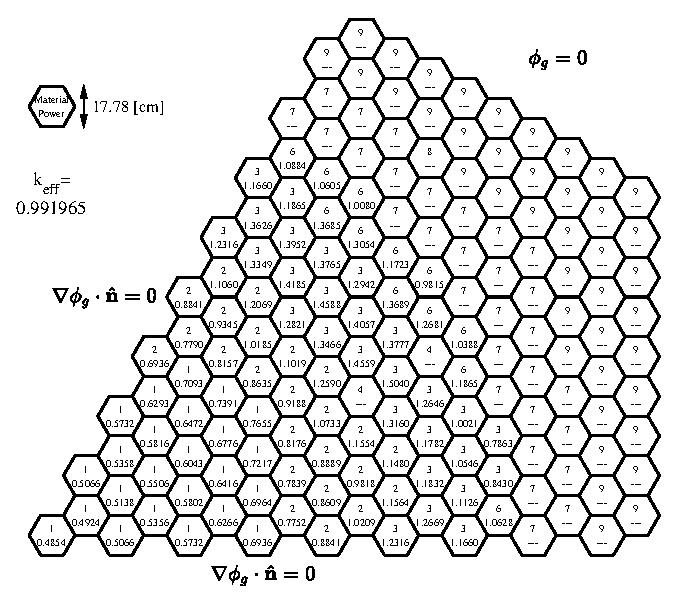
\includegraphics[width=\textwidth]{hwr}
      \caption{\glsentryshort{hwr} Geometry.}
      \label{fig:hwr_geom}
    \end{figure}

    \begin{table}
      \caption{\glsentryshort{hwr} Cross Sections.}
      \label{tab:hwrxs}
      \begin{center}
        \begin{tabular}{cccccc}
          \toprule
          &MAT1&MAT2&MAT3&MAT4&MAT5\\
          \midrule
          $D_1$&1.382500E+00&1.382550E+00&1.374420E+00&1.311980E+00&1.200000E+00\\
          $D_2$&8.975220E-01&8.974900E-01&8.883680E-01&8.799140E-01&9.000010E-01\\
          $\Sigma_{r1}$&1.110580E-02&1.117460E-02&1.062040E-02&1.268800E-02&1.268800E-02\\
          $\Sigma_{r2}$&2.230650E-02&2.238760E-02&1.694650E-02&5.290090E-04&5.300000E-04\\
          $\Sigma_{s 1\rightarrow 2}$&8.164570E-03&8.223780E-03&8.088160E-03&1.231150E-02&1.231150E-02\\
          $ \nu \Sigma_{f1}$&2.262160E-03&2.227500E-03&2.142810E-03&&\\
          $ \nu \Sigma_{f2}$&2.306230E-02&2.268490E-02&2.048870E-02&&\\
          \midrule
          &MAT6&MAT7&MAT8&MAT9&\\
          \midrule
          $D_1$&1.381390E+00&1.305990E+00&1.291930E+00&1.065100E+00&\\
          $D_2$&9.036710E-01&8.372560E-01&8.193410E-01&3.228290E-01&\\
          $\Sigma_{r1}$&1.056310E-02&1.173130E-02&1.191530E-02&2.834620E-02&\\
          $\Sigma_{r2}$&2.190300E-02&4.333040E-03&3.005650E-04&3.334890E-02&\\
          $\Sigma_{s 1\rightarrow
          2}$&7.765680E-03&1.109750E-02&1.155820E-02&2.619800E-02&\\
          $ \nu \Sigma_{f1}$&2.394690E-03&&&&\\
          $ \nu \Sigma_{f2}$&2.662100E-02&&&&\\
          \bottomrule
        \end{tabular}
      \end{center}
    \end{table}

    \begin{table}
      \caption{\glsentryshort{hwr} Fission Spectrum.}
      \label{tab:hwrchi}
      \begin{center}
        \begin{tabular}{cc}
          \toprule
          &Fission Spectrum \\
          \midrule
          $\chi_1$& 1.0 \\
          $\chi_2$& 0.0 \\
          \bottomrule
        \end{tabular}
      \end{center}
    \end{table}

  \subsection{IAEA Hex}
    \label{sec:iaea}
    The IAEA Hex \gls{pwr} is presented with solution by \textcite{chao}. This
    benchmark is based on the two-dimensional IAEA \gls{pwr} benchmark for
    Cartesian geometry. The problem is one-twelfth of a reactor core. This
    benchmark has a total of four cases, with and without a reflector ring added
    to the external core and with the albedo condition set to $\albedo = 0.5$
    and $\albedo = 0.125$. Each assembly has a flat-to-flat measurement of
    ${20.00~\units{cm}}$. In the unreflected case, there are seven 15 assemblies
    across the core diameter. In the reflected case, there are 16 assemblies
    across the core diameter. To the precision of the benchmark, the effective
    neutron multiplication factors for each of the four cases are summarized in
    \tref{tab:iaeakref}. Assembly geometry and powers are provided geometries
    with and without reflector in \fref{fig:iaea_geom}. Two-group cross sections 
    are provided in \tref{tab:iaeaxs}.  Fission spectrum is provided in
    \tref{tab:iaeachi}.

    \begin{table}
      \caption{IAEA Hex Effective Neutron Multiplication Factors.}
      \label{tab:iaeakref}
      \begin{center}
        \begin{tabular}{llc}
          \toprule
          Reflector & albedo ($\albedo$) & $\kref$ \\
          \midrule
          Without & 0.125 & 0.991378 \\
          Without & 0.5   & 0.978077 \\
          With    & 0.125 & 1.006630 \\
          With    & 0.5   & 1.005507 \\
          \bottomrule
        \end{tabular}
      \end{center}
    \end{table}

    \begin{figure}
      \centering
      \subfloat[Unreflected IAEA Hex.]
        {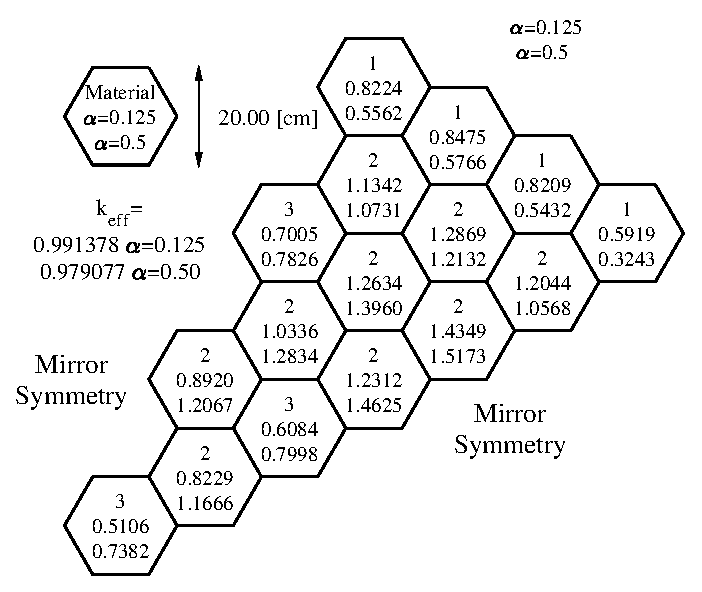
\includegraphics[width=0.65\textwidth]{iaea_nore}}
      \\
      \subfloat[Reflected IAEA Hex.]
        {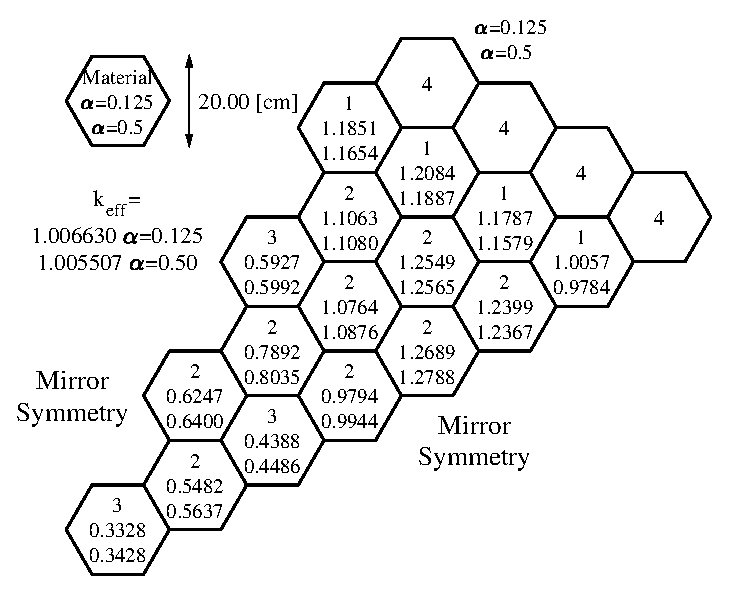
\includegraphics[width=0.65\textwidth]{iaea_refl}}
      \caption{IAEA  Hex Geometry.}
      \label{fig:iaea_geom}
    \end{figure}

    \begin{table}
      \caption{IAEA Hex Cross Sections.}
      \label{tab:iaeaxs}
      \begin{center}
        \begin{tabular}{ccccc}
          \toprule
          &MAT1&MAT2&MAT3&MAT4\\
          \midrule
          $D_1$&1.500001E+00&1.500000E+00&1.500001E+00&1.500000E+00\\
          $D_2$&4.000001E-01&4.000000E-01&4.000001E-01&4.000000E-01\\
          $\Sigma_{r1}$&3.000000E-02&3.000000E-02&3.000000E-02&4.000000E-02\\
          $\Sigma_{r2}$&8.000000E-02&8.500000E-02&1.300000E-01&1.000000E-02\\
          $\Sigma_{s 1\rightarrow 2}$&2.000000E-02&2.000000E-02&2.000000E-02&4.000000E-02\\
          $ \nu \Sigma_{f1}$&0.000000E+00&0.000000E+00&0.000000E+00&\\
          $ \nu \Sigma_{f2}$&1.350000E-01&1.350000E-01&1.350000E-01&\\
          \bottomrule
        \end{tabular}
      \end{center}
    \end{table}

    \begin{table}
      \caption{IAEA Hex Fission Spectrum.}
      \label{tab:iaeachi}
      \begin{center}
        \begin{tabular}{cc}
          \toprule
          &Fission Spectrum \\
          \midrule
          $\chi_1$& 1.0 \\
          $\chi_2$& 0.0 \\
          \bottomrule
        \end{tabular}
      \end{center}
    \end{table}

\section{Three-Dimensional Benchmark Problems}
  For three-dimensional benchmarks, control rod worth measurement is used to
  compare diffusion solution to the benchmark solution. To measure control rod
  worth, three cases are modeled, $\{A,B,C\}$, with control rods fully removed
  in case $A$, partially inserted in case $B$, and fully inserted in case $C$.
  Rod worth is presented in units \units{$\Delta k$} and calculated as 
  \begin{equation}
    \text{Rod Worth}_x~\units{$\Delta k$} = \frac{\keffsub{A} - \keffsub{x}}
      {\keffsub{A} \, \keffsub{x}}
  \end{equation}
  for $x = \{B,C\}$. That is, rod worth is always compared to the case with
  control rods fully removed, case $A$. Additionally, Rod Difference is
  presented in units \units{$\% \Delta$k} as
  \begin{equation}
    \text{Rod Difference}_x~\units{$\% \Delta k$} = (\keffsub{A} - \keffsub{x}) 
      \times 100 \%
  \end{equation}
  for $x = \{B,C\}$.

  \subsection{MONJU}
    \label{sec:monju}
    This benchmark is presented with solution by \textcite{monjuBenchmark}.
    It is based on a prototype \gls{fbr} with hexagonal
    pitch. The reactor has one-third rotational (\textit{not} reflective)
    symmetry. For code packages without rotational boundary conditions, it will
    be necessary to simulate a full core. There are 21 assemblies across the
    core diameter with outer rings being blanket assemblies as shown in
    \fref{fig:monju_geom}. Fuel assemblies are shown axially in
    \fref{fig:monju_assy_geom}. Each assembly has a flat-to-flat measurement of
    ${11.56~\units{cm}}$. Vacuum boundary condition ($\albedo = 0.5$) is applied
    on the core periphery and above and below the reactor. Three-group cross 
    sections are provided in \tref{tab:monjuxs}. No fission spectrum is
    specified in the benchmark. The fission spectrum was estimated and is shown
    in \tref{tab:monjuchi}. In determining this fission spectrum, it was
    observed that the benchmark results are not highly sensitive to the fission
    spectrum.

    The reactor is simulated with three different control rod configurations;
    patterns A, B, and C. In pattern A, all control rods are withdrawn and
    control rod channels are simulated with sodium in the channel for the
    extents of the problem. In pattern B, control rods in rings six and seven
    (shaded in \fref{fig:monju_geom}) are half inserted and all others remain
    with drawn. In pattern C, the control assemblies in rings six and seven that
    were previously half inserted are fully inserted. Control rod withdrawal
    patterns are shown in \fref{fig:monju_cr_geom}.
    
    Reference effective neutron multiplication factors and control rod worths
    are provided in \tref{tab:monjukref}.

    \begin{table}
      \caption{MONJU Effective Neutron Multiplication Factors and Rod Worths.}
      \label{tab:monjukref}
      \begin{center}
        \begin{tabular}{cccc}
          \toprule
          Pattern & $\kref$ & Rod Worth \units{$\Delta k$} & Rod Difference
            \units{$\% \Delta k$} \\
          \midrule
          A & 1.0723 &       & \\
          B & 1.0464 & 0.023 & 2.59 \\
          C & 1.0224 & 0.046 & 4.99 \\
          \bottomrule
        \end{tabular}
      \end{center}
    \end{table}

    \begin{figure}
      \centering
      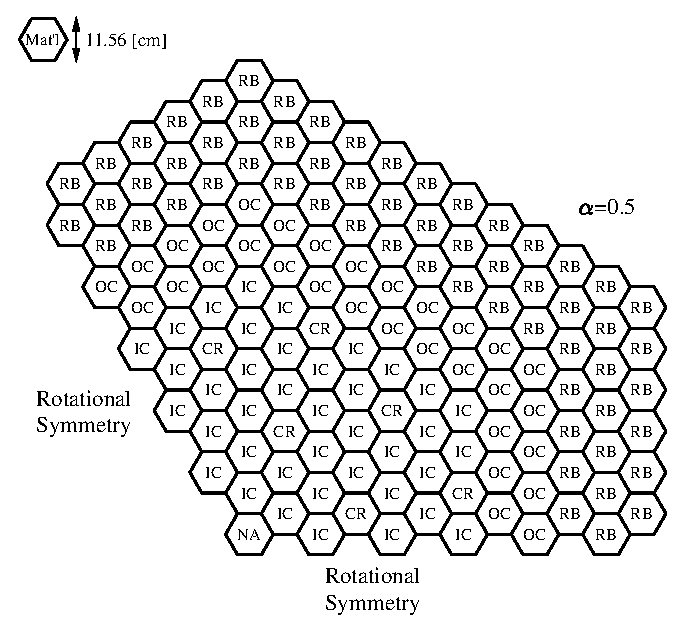
\includegraphics[width=0.7\textwidth]{monju}
      \caption{MONJU Geometry.}
      \label{fig:monju_geom}
    \end{figure}

    \begin{figure}
      \centering
      \subfloat[Assembly Geometry.]{
        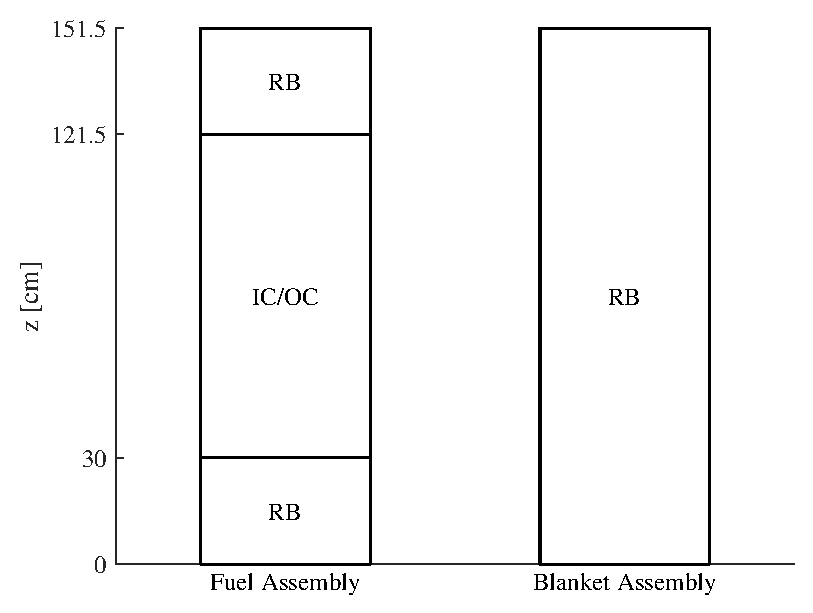
\includegraphics[width=0.45\textwidth]{monju_assembly_geometry}
        \label{fig:monju_assy_geom}}
      \hfill
      \subfloat[Control Rod Geometry.]{
        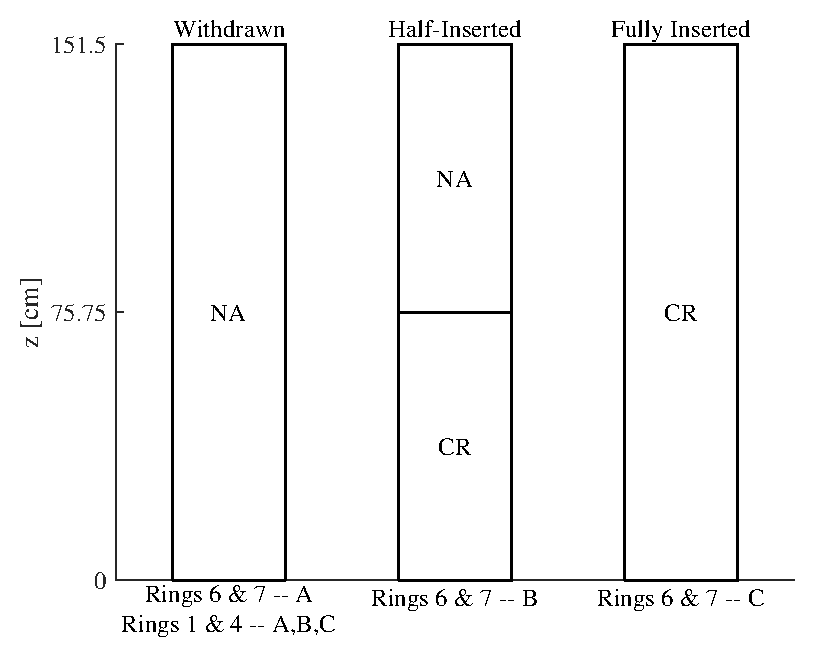
\includegraphics[width=0.45\textwidth]{monju_control_rod_geometry}
        \label{fig:monju_cr_geom}}
      \caption{MONJU Assembly Geometries.}
    \end{figure}

    \begin{table}
      \caption{MONJU Cross Sections.}
      \label{tab:monjuxs}
      \begin{center}
        \begin{tabular}{cccccc}
          \toprule
          &IC&OC&RB&CR&NA\\
          \midrule
          $D_1$&2.540000E+00&2.547990E+00&2.173000E+00&2.500010E+00&4.805000E+00\\
          $D_2$&1.724000E+00&1.725000E+00&1.439000E+00&1.681000E+00&3.262000E+00\\
          $D_3$&1.264000E+00&1.269000E+00&1.026000E+00&1.269000E+00&2.431000E+00\\
          $\Sigma_{r1}$&3.098650E-02&3.121380E-02&3.793080E-02&2.328030E-02&1.152508E-02\\
          $\Sigma_{r2}$&9.490000E-03&9.875000E-03&1.184300E-02&1.272700E-02&3.648740E-03\\
          $\Sigma_{r3}$&7.333000E-03&8.099000E-03&7.611000E-03&1.497000E-02&3.072000E-04\\
          $\Sigma_{s 1\rightarrow 2}$&2.544000E-02&2.497000E-02&3.288000E-02&2.185000E-02&1.130000E-02\\
          $\Sigma_{s 1\rightarrow 3}$&5.625000E-04&5.548000E-04&7.468000E-04&2.163000E-04&6.718000E-05\\
          $\Sigma_{s 2\rightarrow 3}$&6.551000E-03&6.341000E-03&1.000000E-02&9.379000E-03&3.571000E-03\\
          $ \nu \Sigma_{f1}$&1.235000E-02&1.467000E-02&8.631000E-03&&\\
          $ \nu \Sigma_{f2}$&5.225000E-03&6.955000E-03&5.995000E-04&&\\
          $ \nu \Sigma_{f3}$&7.684000E-03&9.986000E-03&1.381000E-03&&\\
          \bottomrule
        \end{tabular}
      \end{center}
    \end{table}

    \begin{table}
      \begin{threeparttable}
        \caption{MONJU Fission Spectrum.}
        \label{tab:monjuchi}
        \begin{tabular}{@{}p{\textwidth}@{}}
          \centering
          \begin{tabular}{cc}
            \toprule
            &Fission Spectrum\tnote{$\dagger$} \\
            \midrule
            $\chi_1$& 0.78120 \\
            $\chi_2$& 0.20994 \\
            $\chi_3$& 0.00886 \\
            \bottomrule
          \end{tabular}
        \end{tabular}
        \begin{tablenotes}
          \centering
          \item[$\dagger$] Estimated values. Not part of original 
            specification.
        \end{tablenotes}
      \end{threeparttable}
    \end{table}

  \subsection{KNK}
    \label{sec:knk}
    This benchmark is presented with solution by \textcite{takedaBenchmark}.  It
    is based on a small \gls{fbr} with hexagonal-z geometry and is a model of
    the KNK-II core. The original benchmark specification is for a transport
    solution, not a diffusion solution. The reactor has one-third rotational
    (\textit{not} reflective) symmetry. For code packages without rotational
    boundary conditions, it will be necessary to simulate a full core. There are
    15 assemblies across the core diameter with outer rings of reflectors and
    steel as shown in \fref{fig:knk_geom}. Fuel assemblies are shown axially in
    \fref{fig:knk_assembly_geom}. Each assembly has a flat-to-flat measurement
    of ${12.99~\units{cm}}$. Vacuum boundary condition ($\albedo = 0.5$) is
    applied on the core periphery and above and below the reactor. Four-group
    cross sections are provided in \tref{tab:knkxs_a} and \tref{tab:knkxs_b}.
    The fission spectrum is provided in \tref{tab:knkchi}.

    The reactor is simulated with three different control rod configurations;
    patterns A, B, and C. In pattern A, all control rods are withdrawn. In
    pattern B, control rods are half inserted into the active fuel region. In
    pattern C, control rods are fully inserted into the active fuel region. All
    axial geometries are shown in \fref{fig:knk_cr_geom}. The axial geometry
    for control rod withdrawal is shown in \fref{fig:knk_cr_geom}.

    Reference effective neutron multiplication factors and control rod worths 
    are provided in \tref{tab:knkkref}.

    The KNK benchmark problem results are presented for the solution to the
    neutron transport equation. The reference presents Monte Carlo solutions and
    other solutions to the neutron transport equation and these converge to
    the same solution. For diffusion solutions to these simulations, agreement
    is expected to within some tolerance. However, comparison can also be
    difficult as the equations solved are entirely different.

    \begin{table}
      \caption{KNK Effective Neutron Multiplication Factors and Rod Worths.}
      \label{tab:knkkref}
      \begin{center}
        \begin{tabular}{cccc}
          \toprule
          Pattern & $\kref$ & Rod Worth \units{$\Delta k$} & Rod Difference
            \units{$\% \Delta k$} \\
          \midrule
          A & 1.0951 &       & \\
          B & 1.9833 & 0.104 & 11.18 \\
          C & 0.8799 & 0.223 & 21.52 \\
          \bottomrule
        \end{tabular}
      \end{center}
    \end{table}

    \begin{figure}
      \centering
      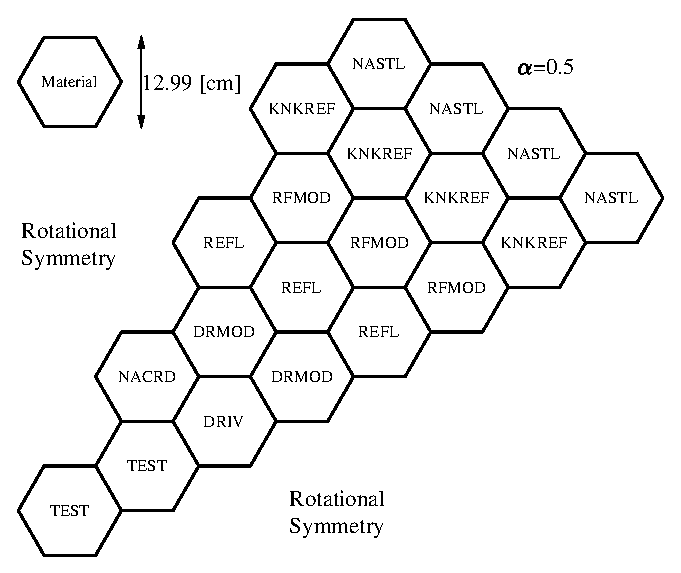
\includegraphics[width=0.7\textwidth]{knk}
      \caption{KNK Geometry.}
      \label{fig:knk_geom}
    \end{figure}

    \begin{figure}
      \centering
      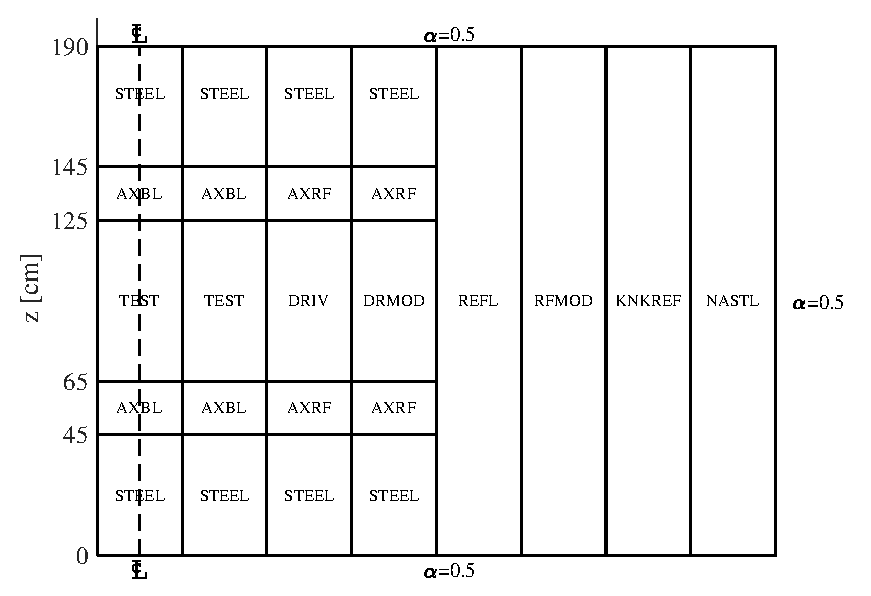
\includegraphics[width=0.7\textwidth]{knk_assembly_geometry}
      \caption{KNK Assembly Geometry.}
      \label{fig:knk_assembly_geom}
    \end{figure}

    \begin{figure}
      \centering
      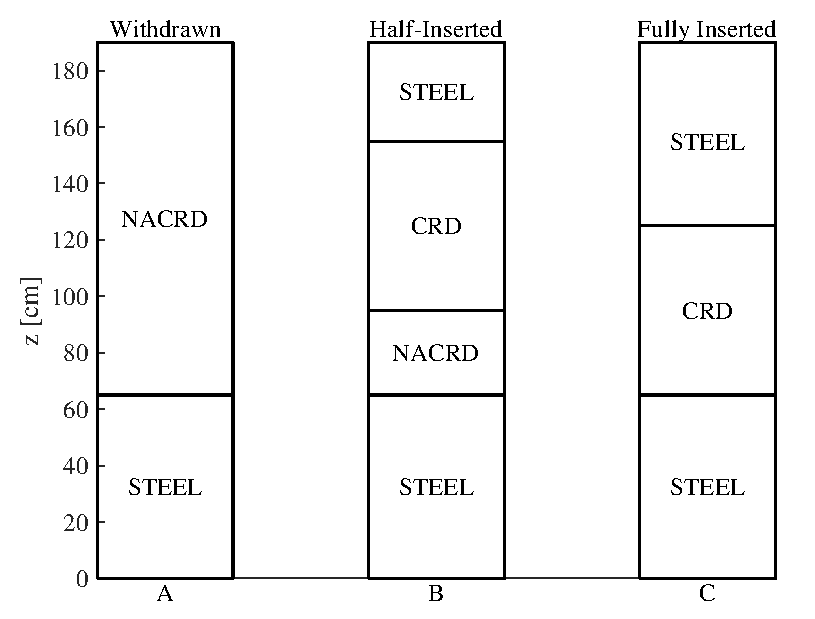
\includegraphics[width=0.7\textwidth]{knk_control_rod_geometry}
      \caption{KNK Control Rod Geometry.}
      \label{fig:knk_cr_geom}
    \end{figure}
    
    \newgeometry{margin=1in,lmargin=1.25in,footskip=\chapterfootskip, includehead, includefoot}
    \thispagestyle{lscapedplain}
    \begin{landscape}
    \begin{table}
      \caption{KNK Cross Sections (Part A).}
      \label{tab:knkxs_a}
      \begin{center}
        \begin{tabular}{cccccccc}
          \toprule
          &STEEL&AXBL&AXRF&TEST&DRIV&DRMOD&REFL\\
          \midrule
          $D_1$&3.388781E+00&2.373121E+00&2.507529E+00&2.676817E+00&2.377115E+00&2.356912E+00&2.091884E+00\\
          $D_2$&2.466578E+00&1.477974E+00&1.867089E+00&1.658169E+00&1.460419E+00&1.358360E+00&1.540678E+00\\
          $D_3$&1.483136E+00&1.019165E+00&1.177228E+00&1.163065E+00&1.023104E+00&8.369847E-01&9.559535E-01\\
          $D_4$&1.177370E+00&9.768754E-01&7.212400E-01&9.039009E-01&7.968248E-01&7.645435E-01&5.339750E-01\\
          $\Sigma_{r1}$&7.758804E-03&1.665700E-02&9.938010E-03&1.856200E-02&2.033901E-02&2.709099E-02&1.137701E-02\\
          $\Sigma_{r2}$&4.558990E-03&8.274010E-03&5.436010E-03&1.165498E-02&1.303201E-02&3.338801E-02&5.945000E-03\\
          $\Sigma_{r3}$&5.202000E-03&9.116980E-03&5.957010E-03&1.639202E-02&1.892099E-02&4.616198E-02&6.607000E-03\\
          $\Sigma_{r4}$&2.410000E-03&9.943000E-03&3.569000E-03&4.981199E-02&5.742100E-02&6.511802E-02&4.942950E-03\\
          $\Sigma_{s 1\rightarrow 1}$&9.060500E-02&1.238050E-01&1.229950E-01&1.059640E-01&1.198870E-01&1.143370E-01&1.479690E-01\\
          $\Sigma_{s 1\rightarrow 2}$&7.423770E-03&1.454830E-02&9.412310E-03&1.127380E-02&1.307900E-02&2.096640E-02&1.066070E-02\\
          $\Sigma_{s 2\rightarrow 2}$&1.305810E-01&2.172600E-01&1.730950E-01&1.893700E-01&2.152130E-01&2.120060E-01&2.104100E-01\\
          $\Sigma_{s 1\rightarrow 3}$&1.181630E-04&1.702760E-04&1.937910E-04&1.461920E-04&1.599380E-04&1.391320E-03&2.499560E-04\\
          $\Sigma_{s 2\rightarrow 3}$&4.352500E-03&6.788850E-03&5.098810E-03&3.648470E-03&4.001170E-03&2.672690E-02&5.467110E-03\\
          $\Sigma_{s 3\rightarrow 3}$&2.195470E-01&3.179480E-01&2.771940E-01&2.702070E-01&3.068850E-01&3.520930E-01&3.420850E-01\\
          $\Sigma_{s 1\rightarrow 4}$&8.258900E-07&9.370830E-07&1.393070E-06&9.621780E-07&1.071660E-06&6.102810E-05&1.825650E-06\\
          $\Sigma_{s 2\rightarrow 4}$&3.416750E-07&6.047930E-06&7.050750E-07&1.068880E-06&1.827160E-06&1.081860E-03&1.001570E-06\\
          $\Sigma_{s 3\rightarrow 4}$&4.645940E-03&4.387820E-03&5.096010E-03&1.804790E-03&1.673410E-03&3.290300E-02&5.368790E-03\\
          $\Sigma_{s 4\rightarrow 4}$&2.807070E-01&3.312810E-01&4.585980E-01&3.189600E-01&3.609060E-01&3.708720E-01&6.193060E-01\\
          $ \nu \Sigma_{f1}$&&2.961000E-03&&1.790430E-02&1.598780E-02&1.016630E-02&\\
          $ \nu \Sigma_{f2}$&&6.561700E-05&&1.599610E-02&1.644460E-02&9.463600E-03&\\
          $ \nu \Sigma_{f3}$&&1.146300E-04&&2.408560E-02&2.714500E-02&1.873250E-02&\\
          $ \nu \Sigma_{f4}$&&4.934825E-04&&7.331050E-02&8.458075E-02&8.253350E-02&\\
          \bottomrule
        \end{tabular}
      \end{center}
    \end{table}
    \end{landscape}
    \restoregeometry
    \pagestyle{plain}

    \newgeometry{margin=1in,lmargin=1.25in,footskip=\chapterfootskip, includehead, includefoot}
    \thispagestyle{lscapedplain}
    \begin{landscape}
    \begin{table}
      \caption{KNK Cross Sections (Part B).}
      \label{tab:knkxs_b}
      \begin{center}
        \begin{tabular}{cccccc}
          \toprule
          &RFMOD&KNKREF&NASTL&CRD&NACRD\\
          \midrule
          $D_1$&2.395256E+00&2.198131E+00&3.453884E+00&2.396616E+00&4.581354E+00\\
          $D_2$&1.349566E+00&2.341120E+00&3.376912E+00&1.461014E+00&3.326083E+00\\
          $D_3$&7.367704E-01&2.018587E+00&2.483855E+00&1.045568E+00&2.074220E+00\\
          $D_4$&6.215936E-01&4.141579E-01&8.077479E-01&5.313220E-01&2.199117E+00\\
          $\Sigma_{r1}$&3.325300E-02&1.321701E-02&8.154706E-03&2.136299E-02&6.395295E-03\\
          $\Sigma_{r2}$&6.217301E-02&4.880000E-03&3.460198E-03&3.345301E-02&4.094401E-03\\
          $\Sigma_{r3}$&7.935300E-02&4.410000E-03&3.444000E-03&7.445399E-02&4.686990E-03\\
          $\Sigma_{r4}$&2.415300E-02&5.912960E-03&3.037990E-03&3.125500E-01&1.207990E-03\\
          $\Sigma_{s 1\rightarrow 1}$&1.059110E-01&1.384270E-01&8.835500E-02&1.177220E-01&6.636340E-02\\
          $\Sigma_{s 1\rightarrow 2}$&2.964850E-02&1.239010E-02&7.734090E-03&1.260660E-02&6.233930E-03\\
          $\Sigma_{s 2\rightarrow 2}$&1.848200E-01&1.375020E-01&9.524930E-02&1.946990E-01&9.612360E-02\\
          $\Sigma_{s 1\rightarrow 3}$&3.065020E-03&3.669300E-04&1.947190E-04&1.333140E-04&7.021210E-05\\
          $\Sigma_{s 2\rightarrow 3}$&5.917800E-02&4.419270E-03&3.225680E-03&4.322190E-03&4.013750E-03\\
          $\Sigma_{s 3\rightarrow 3}$&3.730720E-01&1.607220E-01&1.307560E-01&2.443520E-01&1.560160E-01\\
          $\Sigma_{s 1\rightarrow 4}$&1.416970E-04&1.690360E-06&8.896150E-07&1.088390E-06&4.163880E-07\\
          $\Sigma_{s 2\rightarrow 4}$&2.692290E-03&1.632800E-06&7.984940E-07&1.854910E-07&1.269390E-07\\
          $\Sigma_{s 3\rightarrow 4}$&7.813260E-02&3.330750E-03&2.904810E-03&3.687810E-04&4.491110E-03\\
          $\Sigma_{s 4\rightarrow 4}$&5.121030E-01&7.989320E-01&4.096320E-01&3.148160E-01&1.503680E-01\\
          $ \nu \Sigma_{f1}$&&&&&\\
          $ \nu \Sigma_{f2}$&&&&&\\
          $ \nu \Sigma_{f3}$&&&&&\\
          $ \nu \Sigma_{f4}$&&&&&\\
          \bottomrule
        \end{tabular}
      \end{center}
    \end{table}
    \end{landscape}
    \restoregeometry
    \pagestyle{plain}
    \newgeometry{margin=1in,lmargin=1.25in,footskip=\chapterfootskip, includehead, includefoot}

    \begin{table}
      \caption{KNK Fission Spectrum.}
      \label{tab:knkchi}
      \begin{center}
        \begin{tabular}{cc}
          \toprule
          &Fission Spectrum \\ 
          \midrule
          $\chi_1$&0.908564 \\
          $\chi_2$&0.087307 \\
          $\chi_3$&0.004129 \\
          $\chi_4$&0.000000 \\
          \bottomrule
        \end{tabular}
      \end{center}
    \end{table}


\restoregeometry

%%---------------------------------------------------------------------------%%
%\ensureoddstart
\backmatter

\end{document}
